\documentclass[ngerman,12pt]{article} % alternativ auch document class scrartcl

\usepackage{german}
\usepackage[utf8]{inputenc}
\usepackage[T1]{fontenc} %Deutsche Formatierungen. Zeilenumbrüche, Umlaute..
\usepackage{lmodern}

%\usepackage{pgfplots} % Diagramme wie sin(x)
\usepackage{hyperref}  % Verlinkung in pdf-Dokumenten

\usepackage{listings}  % Quellcode: C++, Pascal und mehr

\usepackage{color}     % Farbe

\usepackage{siunitx}   % SI Einheiten
\sisetup{locale = DE}
\sisetup{output-decimal-marker = {,}}
\sisetup{exponent-product = \cdot} % see siunitx.pdf, table 16 - output options
\sisetup{per-mode=symbol}

\usepackage{amsmath}
\usepackage{amssymb}


% % % % % % % % Maße und Abstände
\usepackage[a4paper]{geometry}
	\geometry{a4paper, top=25mm, left=25mm, right=25mm, bottom=25mm, headsep=10mm, footskip=8mm} % geometry for scientific article
	\setlength{\parindent}{0cm}

% % % % % % % % Headline and Footline
\usepackage{fancyhdr}
	\fancyhf{}
	\pagestyle{fancy}
	\renewcommand{\sectionmark}[1]{\markboth{#1}{}}
	\lhead{\MakeUppercase{\leftmark}} % Headline left
	\chead{}                          % Headline center
	\rhead{\thepage}                  % Headline right
	\lfoot{}                          % Footline left
	\cfoot{}                          % Footline center
	\rfoot{}                          % Footline right
	\renewcommand{\headrulewidth}{0.4pt}
	%\renewcommand{\footrulewidth}{0.4pt}
\usepackage{graphicx}  % Einbinden von Bildern
\usepackage{here} 
\usepackage{subfig}
\usepackage{caption}
\usepackage{tabularx}
\graphicspath{{./Bilder/}}
\sloppy

\begin{document}

%Titelseite
\thispagestyle{empty} 
\begin{center}
{\Large Hochschule Koblenz}\medskip\\
{\Large Fachbereich Ingenieurwesen}\medskip\\
{\Large Elektro- und Informationstechnik}\\[2cm]

\includegraphics[width=5cm]{LogoHS}\\[2cm]
\textbf{Studienarbeit}\\ [0.5cm]
{\LARGE\textbf{Bilddatenvorverarbeitung in einem FPGA}}\\[1ex]
Autor: Lukas Herbst\\
Matrikelnummer: 532903\\
\today\\
Studiengang: Elektrotechnik\\[2cm] 
\end{center}
	\vfill
\begin{tabular}{l@{\hspace{4ex}}l} 
	\textbf{Betreuer:}        & Prof. Dr. Berthold Gick\\
	\textbf{Zeitraum:}        &  26. September 2019 - \today \\
\end{tabular}
\clearpage
\pagenumbering{Roman} % roman page numbers for following pages





%Kurzzusammenfassung
\lhead{Kurzzusammenfassung}
\section*{Kurzzusammenfassung}
In dieser Studienarbeit wird das Thema der \textit{Bildatenvorverarbeitung in einem FPGA} behandelt. Dabei werden Kamerabilder von einem FPGA-Board aufgenommen, gespeichert und weiterverarbeitet. Die Aufgabe bestand darin, aufbauend auf bereits vorhandenen Funktionen, der Speicherung von Kamerabildern und deren Ausgabe über VGA auf einen Monitor, die Bilddatenverarbeitung im FPGA-Board weiterzuentwickeln.\newline

Ziel war es, eine eindimensionale Positionserkennung von Objekten zu implementieren, welche die Erkennung von Punkten und Linien in einer Bildzeile umfasst. Des Weiteren sollte die Bildwiederholungsrate erhöht werden.\\
Zur Erkennung von Objekten in eindimensionalen Bildern wurden verschiedene Funktionsblöcke in der Hardwarebeschreibungssprache Very High Speed Integrated Circuit Hardware Description Language geschrieben. Mittels dieser Funktionsblöcke ist es möglich, Punkte und Linien als Objekte in einer Bildzeile zu erkennen und ihre Position zu ermitteln. Zudem wurde die Bildwiederholungsrate erhöht und die damit verbundenen auftretenden Probleme gelöst.

\clearpage





% Erklärung, das Arbeit eigenständig gemacht wurde
\section*{Eigenständigkeitserklärung}
Ich habe die vorliegende Arbeit selbständig verfasst und keine anderen als die angegebenen Quellen und Hilfsmittel benutzt.
Wörtlich oder sinngemäß übernommenes Gedankengut habe ich als solches kenntlich gemacht.
\footnote{
Dies ist keine \glqq Eidesstattliche\grqq\ Erklärung, da i.d.R. keine Vereidigung stattgefunden hat.}

\vspace*{3cm}\noindent
\parbox{6cm}{\hrulefill\\\centering(Ort, Datum)}
\hfill
\parbox{6cm}{\hrulefill\\\centering(Unterschrift)}
\clearpage





%Inhaltsverzeichnis
%\addcontentsline{toc}{section}{Inhaltsverzeichnis}
\lhead{Inhaltsverzeichnis} %erzeugt Kopfzeile
\tableofcontents %erzeugt Inhaltsverzeichnis
\clearpage





% Abbildungsverzeichnis
\lhead{Abbildungsverzeichnis}
\addcontentsline{toc}{section}{Abbildungsverzeichnis}  % Add entry to table of contents
\listoffigures % Abbildungsverzeichnis
\clearpage





% Tabellenverzeichnis
\addcontentsline{toc}{section}{Tabellenverzeichnis} % Add entry to table of contents
\lhead{Tabellenverzeichnis}
\listoftables % Tabellenverzeichnis
\clearpage





% Abkürzungsverzeichnis
\section*{Abkürzungsverzeichnis} % no section number, no entry in table of contents
\lhead{Abkürzungsverzeichnis}
\addcontentsline{toc}{section}{Abkürzungsverzeichnis} % Add entry to table of contents

\begin{tabular}{@{\bf}ll}
	AIA	&Automated Imaging Association\\
	AS	&Active Serial\\
	ASCI	&Application Specific Integrated Circuit\\
	CBL	& konfigurierbarer Logikblock\\
	CLR-HSMC	&Camera Link Receiver High Speed Mezzanine Card\\ 
	EEPROM	& Electrically Erasable Programmable Read Only Memory\\
	FIFO	&FirstInFirstOut\\
	FPGA	&Field Programmable Gate Array \\
	FPS	&Frames per Second\\
	I/O	&Input/Output\\
	LUT	&Look UP Table\\
	LVDS	&Low Voltage Differential Signaling\\
	PLD	&Programmable Logic Device\\
	PLL	&Phase Locked Loop\\
	pof	&Programmer Object File\\
	RAM	&Random Access Memory\\
 	RS	&Recommended Standard\\
	SDR 	&Shrunk Delta Ribbon\\
	sof	&SDRAM Object File\\
	VGA	&Video Graphics Array\\
	VHDL	&Very High Speed Integrated Circuit Hardware Description Language \\
\end{tabular}
\clearpage





\lhead{\leftmark}
\pagenumbering{arabic}%arabic page numbers for following pages

% Einleitung Anfang
\section{Einleitung}
\label{sec:Einleitung}
Die digitale Bilddaten(vor)verarbeitung nutzt Bilder, die aus verschiedenen Bereichen des elektromagnetischen Spektrums stammen. Das genutzte elektromagnetische Spektrum reicht vom Gamma- und Röntgenstrahlenbereich über den Bereich des ultravioletten, sichtbaren und infraroten Lichtes bis in den Mikro- und Radiowellenbereich. Zudem gibt es neben Bildern im elektromagnetischen Spektrum auch akustische und computergenerierte Bilder sowie die Elektronenmikroskopie.\\
Anwendungsbereiche für digitale Bildverarbeitung lassen sich u.a. in der Industrie, Medizin, Astronomie, Geografie und der Wetterüberwachung finden. So werden in der Industrie Röntgenstrahlen genutzt, um z.B. Bilder von Platinen aufzunehmen, damit auf diese Weise Produktionsmängel entdeckt werden können, wie etwa fehlende Bauteile. Zudem wird dort der sichtbare Bereich genutzt, um Objekte bzw. Fehler in Objekten, wie Lufteinschlüsse, zu erkennen oder die Postionen von Objekten zu bestimmen. In der Medizin werden Gammastrahlen für die Emissionscomputertomographie, Röntgenstrahlen für Röntgenbilder, Radiowellen für die Magnetresonanztomographie und Ultraschallwellen für Ultraschallbilder genutzt \cite{Gonzalez}.\newline

Diese Arbeit beschäftigt sich vorrangig mit dem Anwendungsbereich der Positionserkennung von Objekten im Bereich des sichtbaren Lichts. Dabei werden Bilder mittels einer Kamera aufgenommen und in einem Field Programmable Gate Array - Board (FPGA-Board) verarbeitet. Dabei baut diese Arbeit auf bereits vorhandenen bildverarbeitenden Funktionen im FPGA-Board auf. Zu Bearbeitungsbeginn der Studienarbeit war es möglich, die Daten der Kamerabilder mittels Camera Link von der Kamera auf das FPGA-Board zu übertragen und diese dort zwischenzuspeichern. Diese zwischengespeicherten Daten konnten über den VGA-Ausgang auf einem angeschlossenen Monitor ausgegeben werden.\\
Auf Basis der zuvor bereits beschriebenen laufenden Funktionen werden neue Funktionen auf dem FPGA-Board implementiert. Die Implementierung dieser Funktionen zur Positionserkennung von Objekten wird schrittweise durchgeführt. Zuerst erfolgt die Positionserkennung eindimensional in einem Schwarzweißbild. Anschließend wird die eindimensionale Positionserkennung auf mehrere Objekte erweitert. Danach erfolgt die Erhöhung der Bildwiederholungsrate.\\
Darauf aufbauend kann eine Positionserkennung für ein zweidimensionales Objekt in einem Schwarzweißbild implementiert werden, d.h., dass im gesamten Bild oder in einem mehrere Zeilen großen Bildausschnitt ein Objekt gesucht. Dies kann anschließend auf die Erkennung der Position mehrerer Objekte ausgeweitet werden. Durch die Positionserkennung eines oder mehrerer Objekte soll es später möglich sein, die Beschleunigung und Geschwindigkeit eines Objektes zu erfassen. Die Daten der Beschleunigung und Geschwindigkeit können dann für die Ansteuerungen der Bewegung dieser Objekte genutzt werden.\newline

In Kapitel \ref{sec:Digitale Bildverarbeitung} wird darauf eingegangen, was ein digitales Bild und digitale Bildverarbeitung sind. Zudem werden Zusammenhänge zwischen benachbarten Pixeln erläutert und mathematische Bildoperationen zur Kanten- und Objekterkennung beschrieben.\\
Darauf folgend wird in Kapitel \ref{sec:FPGA-Board und Hardwarebeschreibung} auf die bildverarbeitende Komponente(FPGA-Board) sowie die Möglichkeit, die Hardwarebeschreibung durchzuführen.\\
Kapitel \ref{sec:Aufbau und Hardwarekomponenten} beschreibt den Aufbau und die Funktion der genutzten Hardwarekomponenten der Studienarbeit.\\
Danach wird in Kapitel \ref{sec:Stand zu Bearbeitungsbeginn} der Stand des Projekts, auf dem die Weiterentwicklung der Bilddatenverarbeitung während der Studienarbeit beruht, beschrieben.\\
Auf diesen Stand aufbauend, wird in Kapitel \ref{sec:Eindimensionale Positionserkennung} das Extrahieren einer Bildzeile aus einem Bild beschrieben und die eindimensionale Positionserkennung in dieser Zeile erläutert.\\
In Kapitel \ref{sec:Bildwiederholungsrate} wird die Erhöhung der Bildwiederholungsrate und deren Auswirkung auf die eindimensionale Positionserkennung eingegangen.\\
Anschließend werden in Kapitel \ref{sec:Ergebnis und Diskussion} die erzielten Ergebnisse dargestellt und bewertet.\\
Abschließend wird in Kapitel \ref{sec:Zusammenfassung und Ausblick} die Ergebnisse der Arbeit zusammengefasst und ein Ausblick auf zukünftige Arbeiten gegeben.\\
\clearpage
%Einleitung Ende





%Grundlagen Anfang
%Digitale Bildverarbeitung Anfang
\section{Digitale Bildverarbeitung}
\label{sec:Digitale Bildverarbeitung}
Die digitale Bilddaten(vor)verarbeitung umfasst die Aufnahme und Verarbeitung digitaler Bilder. Im Nachfolgenden wird erläutert, wie ein digitales Bild aufgebaut ist und wie die Grenzen zwischen den einzelnen Stufen der Bildverarbeitung verteilt sind. Zudem wird auf die Beziehungen zwischen Pixeln und mathematischen Anwendungsmethoden zur Verarbeitung digitaler Bilder eingegangen.



\subsection{Digitales Bild und digitale Bilddaten(vor)verarbeitung}
\label{sec:Digitales Bild und digitale Bilddaten(vor)verarbeitung}
Die digitale Bilddaten(vor)verarbeitung ist eine Methode, digitale Bilder zu bearbeiten und aus diesen Informationen zu gewinnen. Dabei wird ein Bild als zweidimensionale Funktion f(x,y) beschrieben, bei der die x-Koordinate die Spalte und die y-Koordinate die Zeile eines Bildes beschreibt, wie es in \autoref{pic:Aufbau digitales Bild} dargestellt ist. Die Amplitude der Funktion f(x,y) ist die Intensität bzw. Graustufe des Bildes an diesen Koordinaten. Ein Bild wird als digitales Bild bezeichnet, wenn x, y und die Amplitude der Funktion einer finiten und diskreten Menge entstammen. Diese digitalen Bilder bestehen somit aus einer endlichen Anzahl an Elementen, die meist Pixel genannt werden \cite{Gonzalez}.\\

\begin{figure} [h!tb]
	\begin{center}
	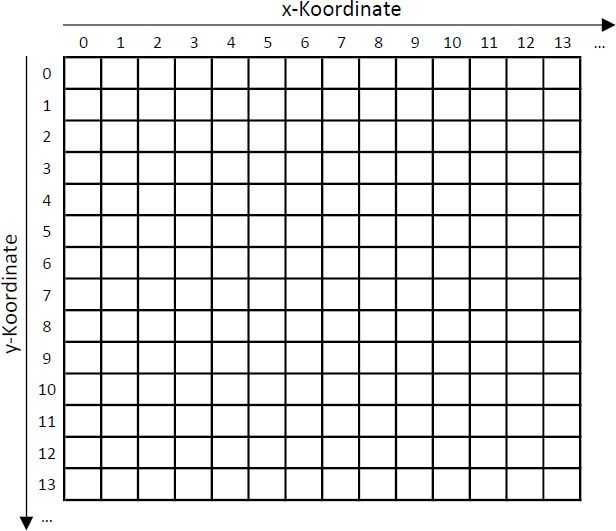
\includegraphics[width=0.5\textwidth]{Aufbau digitales Bild}
	\caption[Aufbau eines digitalen Bildes]{\label{pic:Aufbau digitales Bild}Aufbau eines digitalen Bildes}
	\end{center}
\end{figure}

Gonzalez definiert die digitale Bildverarbeitung als Verarbeitung von Bildern, bei der der Input ein digitales Bild ist und der Output ein digitales Bild oder aus diesem Bild extrahierte Eigenschaften. Diese Eigenschaften dienen zur Wiedererkennung individueller Objekten. Die Schritte der digitalen Bilddatenverarbeitung sind der Erwerb eines Bildes, dessen Vorverarbeitung, das Extrahieren des Charakters, die Beschreibung des Charakters für die Verarbeitung in einem Computer und die Wiedererkennung des Charakters.\\
Da es keine klar definierte Abgrenzung zwischen digitaler Bildverarbeitung und künstlichen/virtuellen Sehens (computer vision) gibt, unterteilt Gonzalez diese in drei Stufen des Verarbeitungsgrades, um eine Abgrenzung dieser zwei Bereiche zu finden. Diese Stufen sind der \textit{low-level process}, der \textit{mid-level process} und der \textit{high-level process}. Im \textit{low-level process} findet die Bilddatenvorverarbeitung statt, die u.a. die Reduktion von Störungen, Kontrastverbesserung und Schärfung umfasst. Der \textit{mid-level process} umfasst die Segmentierung eines digitalen Bildes in Teilbilder und Objekte und die Aufbereitung dieser, um sie für die Verarbeitung mittels Computer nutzen zu können. Der \textit{high-level process} beschäftigt sich mit dem \textit{Sinngeben} der erkannten Objekte, das der Wahrnehmung und Verarbeitung des menschlichen Sehens sehr nahe kommt.



\subsection{Beziehungen zwischen Pixeln}
\label{sec:Beziehungen zwischen Pixeln}
Auf Basis der Definition eines digitalen Bildes als Funktion f(x,y) wird in diesem Abschnitt auf die Beziehungen der Pixel eines digitalen Bildes zueinander eingegangen.\\

\begin{figure} [h!tb]
	\begin{center}
	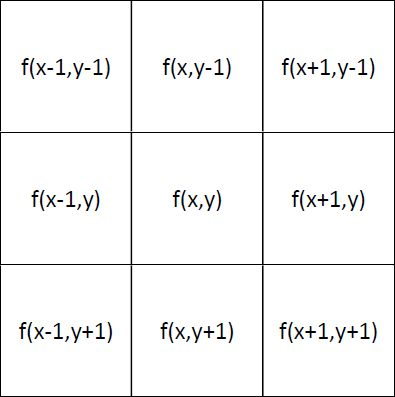
\includegraphics[width=0.2\textwidth]{Pixel p f(x,y)}
	\caption[Pixel p f(x,y)]{\label{pic:Pixel p f(x,y)}Pixel p f(x,y)}
	\end{center}
\end{figure}

So hat ein Pixel p an der Stelle f(x,y) laut Gonzalez zwei vertikale (f(x+1,y), f(x-1,y)), zwei horizontale (f(x,y+1), f(x,y-1)) und 4 diagonale (f(x+1,y+1), f(x+1,y-1), f(x-1,y+1), f(x-1, y-1)) Nachbarn. Diese benachbarten Pixel des Pixels p sind in \autoref{pic:Pixel p f(x,y)} dargestellt. Zudem werden die Nachbarpixel von p, wie in \autoref{pic:4,D,8 Nachbarpixel} gezeigt, in drei verschiedene Gruppen von Nachbarn eingeteilt. Die zwei vertikalen und die zwei horizontalen sind die N\textsubscript{4}(p) und die vier diagonalen sind die N\textsubscript{D}(p) Nachbarpixel. Alle Pixelnachbarn zusammen werden als N\textsubscript{8}(p) Nachbarpixel bezeichnet.\\

\begin{figure}[h!tb]
  \centering
  \subfloat[ ][ ]{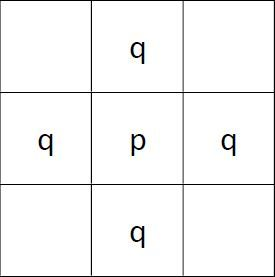
\includegraphics[width=0.2\textwidth]{N4_Nachbarpixel}}
  \qquad
  \subfloat[ ][ ]{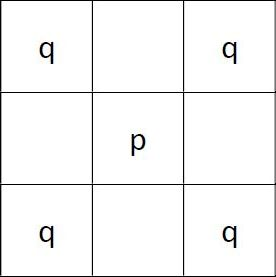
\includegraphics[width=0.2\textwidth]{ND_Nachbarpixel}}
  \qquad
  \subfloat[ ][ ]{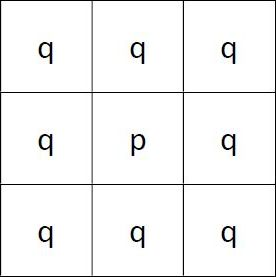
\includegraphics[width=0.2\textwidth]{N8_Nachbarpixel}}
 \caption[Darstellung der  N\textsubscript{4}(p), N\textsubscript{D}(p) und  N\textsubscript{8}(p) Nachbarn des Pixels p]{\label{pic:4,D,8 Nachbarpixel}Darstellung der N\textsubscript{4}(p) (a), N\textsubscript{D}(p) (b) und  N\textsubscript{8}(p) (c) Nachbarn des Pixels p}
\end{figure}

Des Weiteren definiert Gonzalez drei verschiedene Nachbarschaftsarten, bei denen zwei Pixel p und q nur unter bestimmten Voraussetzungen als benachbart gelten. Dies ist zum einen die 4-Nachbarschaft, bei der die zwei Pixel p und q benachbart sind, wenn ihre Intensitäten aus einer gemeinsamen Menge V entspringen und q gleichzeitig ein N\textsubscript{4}(p) Nachbar ist. Zum anderen gibt es die 8-Nachbarschaft, bei der die Pixel p und q benachbart sind, wenn ihre Intensitäten aus V stammen und q ein N\textsubscript{8}(p) Nachbar ist. Die dritte Art der Nachbarschaft ist die m-Nachbarschaft. Hierbei sind die Pixel p und q benachbart, wenn p und q Intensitätswerte aus V haben und sie N\textsubscript{4}(p) Nachbarn sind oder es handelt sich um N\textsubscript{D}(p) Nachbarn, deren Pixel N\textsubscript{4}(p) \(\wedge\)  N\textsubscript{4}(q) Intensitäten haben müssen, die nicht aus der Menge V stammen. Die Beispiele in \autoref{pic:Nachbarschaftsarten zwischen zwei Pixeln} a, b und c zeigen die verschiedenen Nachbarschaftsarten. Dabei wird davon ausgegangen, dass die Intensität der Pixel aus der Menge $ V =\{1\}$ stammen müssen, um benachbart zu sein. Ob zwei Pixel benachbart sind, wird durch die schwarze Linie zwischen den Pixeln gezeigt.\newline

\begin{figure}[h!tb]
  \centering
  \subfloat[ ][ ]{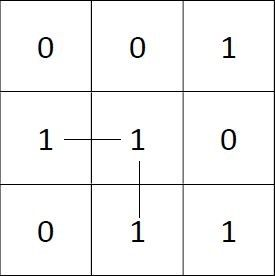
\includegraphics[width=0.2\textwidth]{4_Nachbarschaftsart}}
  \qquad
  \subfloat[ ][ ]{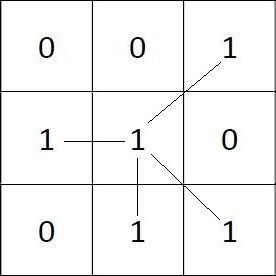
\includegraphics[width=0.2\textwidth]{8_Nachbarschaftsart}}
  \qquad
  \subfloat[ ][ ]{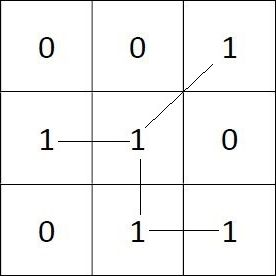
\includegraphics[width=0.2\textwidth]{m_Nachbarschaftsart}}
 \caption[Darstellung der 4-, 8- und m-Nachbarschaftsart]{\label{pic:Nachbarschaftsarten zwischen zwei Pixeln}Darstellung der 4- (a), 8- (b) und m-Nachbarschaftsart (c); benachbarte Pixel sind durch einen schwarzen Strich miteinander verbunden}
\end{figure}

Neben den verschiedenen Nachbarschaftsarten kann ein digitales Bild zusätzlich in verschiedene Teilmengen unterteilt werden. Die beiden Mengen S und R sind Teilmengen von Pixeln aus einem digitalen Bild. Dabei sind zwei Pixel p und q in der Teilmenge S miteinander verbunden, wenn es einen digitalen Pfad zwischen diesen beiden Pixeln gibt, wobei die Pixel des Pfades auch aus der Teilmenge S stammen müssen. Ein digitaler Pfad ist laut Gonzalez ein Pfad zwischen einem Pixel p mit den Koordinaten (x\textsubscript{0},y\textsubscript{0}) und einem Pixel q mit den Koordinaten (x\textsubscript{n},y\textsubscript{n}), wobei die einzelnen Pixel des Pfades eine 4-,8- oder m-Nachbarschaft aufweisen müssen, je nachdem welche Nachbarschaftsart für den digitalen Pfad gewählt wurde. Zudem ist ein digitaler Pfad ein geschlossener Pfad, wenn der Endpunkt dem Ausgangspunkt entspricht. Die Teilmenge R, die auch Region eines Bildes genannt wird, ist eine verbundene Menge von Pixeln mit Intensitäten aus der Menge V. Zwei Regionen R\textsubscript{i} und R\textsubscript{j} sind je nach gewählter Nachbarschaftsart benachbart, wenn mindestens ein Pixel aus R\textsubscript{i} mit einem Pixel aus R\textsubscript{j} benachbart ist. Die innere Grenze einer Region bilden die Pixel von R, die neben Pixeln liegen, die nicht zur Region R gehören. Die äußere Grenze bilden die Pixel, die die Region R umschließen.



\subsection{Mathematische Operationen zur Bilddatenverarbeitung}
\label{sec:Mathematische Operationen zur Bilddatenverarbeitung}
Mithilfe von mathematischen Operationen können aus den Bilddaten Informationen über das Bild erlangt werden. Nach Gonzalez ist es möglich, anhand des Ergebnisses der 1. (\autoref{eq:erste Ableitung}) und 2. (\autoref{eq:zweite Ableitung}) Ableitung der eindimensionalen Funktion f(x), die ein eindimensionales Bild beschreibt, Unterschiede zwischen benachbarten Pixeln zu erkennen. Dies sind zum Beispiel sprunghafte oder rampenförmige Intensitätswechsel, mit deren Hilfe Objekte erkannt werden können. 

\begin{align}
\label{eq:erste Ableitung}
	\frac{\partial{f}} {\partial{x}} = f(x+1) - f(x)
\end{align}
\begin{align}
\label{eq:zweite Ableitung}
	\frac{\partial^2{f}} {\partial^2{x}} = f(x+1)  - 2 f(x) + f(x-1)
\end{align}

Aus der 1. und 2. Ableitung kann jeweils eine Gewichtungsmatrix (\autoref{pic:Matrizen aus 1. und 2. Ableitung} a und b) abgeleitet werden. Mithilfe dieser Gewichtungsmatrix kann eine Faltung mit den Pixelwerten einer Zeile durchgeführt werden. Anhand der Ergebnisse der Faltung für jedes Pixel einer Zeile kann darauf geschlossen werden, wie sich ein Pixel in seiner Intensität zu seinen Nachbarpixeln verhält.

\begin{figure}[h!tb]
  \centering
  \subfloat[ ][ ]{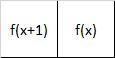
\includegraphics[width=0.15\textwidth]{1te_Ableitung_Matrix_1_gedreht}}
  \qquad
  \subfloat[ ][ ]{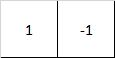
\includegraphics[width=0.15\textwidth]{1te_Ableitung_Matrix_2_gedreht}}
  \qquad
  \subfloat[ ][ ]{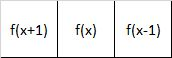
\includegraphics[width=0.225\textwidth]{2te_Ableitung_Matrix_1_gedreht}}
  \qquad
  \subfloat[ ][ ]{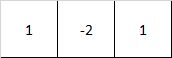
\includegraphics[width=0.225\textwidth]{2te_Ableitung_Matrix_2}}
  \caption[Matrizen aus 1. und 2. Ableitung eines Bildpunktes f(x) ]{\label{pic:Matrizen aus 1. und 2. Ableitung}Matrizen aus 1. (a, b) und 2. Ableitung (c, d) eines Bildpunktes f(x) zur Gewichtung der einzelnen Faltungselementen}
\end{figure}

Die oben erwähnte mathematische Operation der Faltung dient zur Gewichtung der einzelnen Elemente einer Funktion und ist beispielhaft in \autoref{pic:Faltung_Beispiel_Durchführung} gezeigt. Dort wird eine Folge von Pixelwerten mit der Gewichtungsmatrix der 2. Ableitung aus \autoref{pic:Matrizen aus 1. und 2. Ableitung} d gefaltet. Dabei wird zuerst eine der beiden Funktionen in der Mitte gespiegelt; dies ist hier mit der Gewichtungsmatrix an der Stelle \textit{-2} geschehen. Da sich die Werte 1, -2 und 1 allerdings symmetrisch um verteilen, entsteht eine Gewichtungsmatrix, die genauso aussieht wie die Ausgangsmatrix. Anschließend wird das Ergebnis der Faltung für die Startposition berechnet, indem die Elemente der Gewichtungsmatrix mit überschneidenden Pixelwerten multipliziert und aufsummiert werden. Das Ergebnis dieser Berechnung beträgt 0 und wird in der Zeile \textit{Ergebnis} an die Stelle des mittleren Elementes der Gewichtungsmatrix geschrieben. Anschließend wird die Gewichtungsmatrix ein Feld weiter geschoben (1. Verschiebung). Dort werden die Elemente der Gewichtungsmatrix erneut mit den überschneidenden Pixelwerten multipliziert und aufsummiert. Das Ergebnis wird wieder an die Stelle des mittleren Elementes der Gewichtungsmatrix in die Zeile \textit{Ergebnis} geschrieben. Dieser Vorgang wird solange wiederholt, bis die in der \autoref{pic:Faltung_Beispiel_Durchführung} beschriebene Endposition erreicht ist. In der Zeile \textit{Ergebnis} steht nun das Ergebnis der Faltung aller Pixelwerte mit der Gewichtungsmatrix.\newline

\begin{figure} [h!tb]
	\begin{center}
	\includegraphics[width=0.6\textwidth]{Faltung_Beispiel_Durchführung}
	\caption[Durchführung einer Faltung]{\label{pic:Faltung_Beispiel_Durchführung}Beispiel der Durchführung einer Faltung mit der Gewichtungsmatrix der 2. Ableitung}
	\end{center}
\end{figure}

Wie bereits erläutert, kann das Ergebnis der Faltung aus einer Gewichtungsmatrix und den Pixelwerten einer Zeile auf Intensitätsunterschiede zwischen benachbarten Pixeln hinweisen. Dies ist beispielhaft in \autoref{pic:Faltung_Beispiel_Ergebnis} dargestellt. In dieser Abbildung ist das Ergebnis der Faltung von Pixelwerten einer Zeile, die einen Wert zwischen 0 und 10 annehmen können, mit der Gewichtungsmatrix der 1. und der 2. Ableitung dargestellt.\\
Diese Zeile weist von der x-Koordinate f(x) bis zur x-Koordinate f(x+2) als erstes eine Folge von Pixeln mit dem gleichen Intensitätswert, der 10 beträgt, auf. Danach folgt eine rampenförmige Abnahme der Intensität, bis diese den Wert 0 an der Stelle f(x+7) erreicht und die nächsten zwei Pixel den Wert 0 haben. Danach erfolgt von f(x+9) zu f(x+10) ein Sprung mit einem Intensitätswechsel von 0 auf 10. Anschließend haben die Pixel den Intensitätswert 10, außer an der Stelle f(x+13). Dort ist ein isolierter Punkt zu sehen.\\
Ein Punkt ist ein isolierter Punkt, wenn er sich in seiner Intensität stark von seinen Nachbarpixeln unterscheidet.\\

\begin{figure} [h!tb]
	\begin{center}
	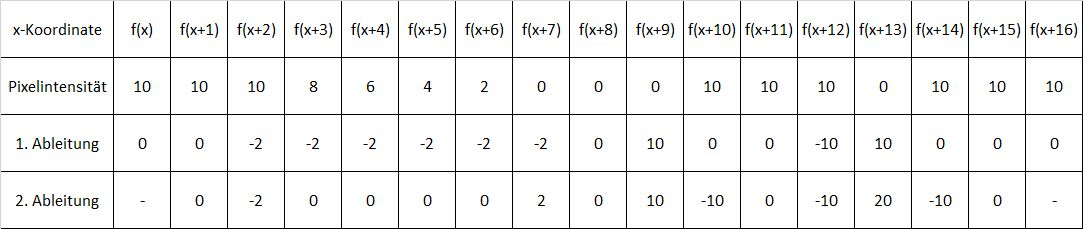
\includegraphics[width=1\textwidth]{Faltung_Beispiel_Ergebnis}
	\caption[Folge von Pixeln mit Ergebnis der 1. und 2. Ableitung]{\label{pic:Faltung_Beispiel_Ergebnis}Folge von Pixelwerten und Ergebnisse der 1. und 2. Ableitung für alle x-Koordinaten}
	\end{center}
\end{figure}

Die beschriebenen Formen des Intensitätswechsels (Folgen gleicher Intensität, Rampen, Sprünge und isolierte Punkte) lassen sich anhand der Ergebnisse der Faltung mit der 1. und 2. Ableitung bestimmen. So ergibt das Ergebnis der 1. Ableitung 0, wenn sich ein Pixel in seiner Intensität nicht von seinem nachfolgenden Pixel unterschiedet, wie es bei den Pixeln an den x-Koordinaten f(x) und f(x+1) zu sehen ist. Unterscheiden sich die Intensitätswerte zwei aufeinander folgender Pixel, so ist das Ergebnis ungleich 0. Eine Folge von Nullen als Ergebnis der 1. Ableitung weist auf eine Folge von Pixeln mit gleicher Intensität hin (f(x) bis f(x+1)). Der Beginn einer Rampe ist durch ein Ergebnis ungleich 0 erkennbar und entlang einer Rampe ist das Ergebnis ebenfalls ungleich 0, wie es an Werten der 1. Ableitung von der Stelle f(x+2) bis f(x+7) zu erkennen ist. Ein Sprung in der Intensität ist daran auszumachen, dass die 1. Ableitung an der Stelle vor dem Sprung einen großen Wert aufweist, wie das Ergebnis für die Pixel f(x+9) und f(x+10) zeigt, an denen ein Intensitätswechsel von 0 auf 10 stattfindet. Danach folgt an der x-Koordinate f(x+13) ein isolierter Punkt, der sich durch einen betragsmäßig großen Wert als Ergebnis der 1. Ableitung am vorherigen Pixel f(x+12) und einem großen Wert mit invertiertem Vorzeichen an seiner Koordinate bemerkbar macht.\\
Für die 2. Ableitung kann an der Stelle f(x) kein Ergebnis für die Faltung berechnet werden, da drei Pixelwerte für die Berechnung benötigt werden. Dies gilt ebenfalls für das letzte Pixel f(x+16) der Zeile. Eine Folge von Pixeln mit gleicher Intensität hat das Ergebnis 0, wie es an der Stelle f(x+1) zu sehen ist. Ein rampenförmiger Intensitätswechsel kündigt sich mit einem Ergebnis für die 2. Ableitung an, welches ungleich 0 ist, folgend von Ergebnissen gleich 0 entlang der Rampe und einen Ergebnis ungleich 0 am Ende der Rampe, welches aber ein invertiertes Vorzeichen im Vergleich zum Ergebnis des Beginns der Rampe aufweist. Dies ist von der Stelle f(x+2) bis f(x+7) mit dem Wert -2 am Beginn und dem Wert 2 am Ende der Rampe zu erkennen. Ein Sprung in der Intensität ist dadurch zu erkennen, dass die Faltung mit der 2. Ableitung ein Ergebnis ungleich 0 an der Stelle vor dem Sprung und ein Ergebnis ungleich 0 mit invertiertem Vorzeichen an der Stelle des Sprungs vorweist. Dies ist an den Ergebnissen für die Stellen f(x+9) und f(x+10) zu erkennen. Dort findet in der Pixelintensität ein Sprung von 0 auf 10 statt und das Ergebnis der 2. Ableitung beträgt an diesen Stellen 10 und -10. Der sich an der x-Koordinate f(x+13) befindliche isolierte Punkt ist daran zu erkennen, dass er an dieser Stelle einen großen Wert ungleich 0 vorzuweisen hat und dass seine Nachbarpixel Werte ungleich 0 mit invertiertem Vorzeichen besitzen.\\
Je größer der Betrag des Ergebnisses der 1. oder 2. Ableitung ist, desto größer sind auch die Intensitätsunterschiede bei Rampen, Sprüngen oder isolierten Punkten. Mittels der Berechnung der Faltung der Gewichtungsmatrix von der 1. oder 2. Ableitung mit den Pixelwerten und eines Auswertungsalgorithmus ist es möglich, Objekte zu erkennen und deren Position in einer Zeile zu bestimmen.\\

Mittels der Laplace-Operation (\autoref{eq:Laplace-Operation-1} und \autoref{eq:Laplace-Operation-2}), die einer 2. Ableitung einer zweidimensionalen Funktion f(x,y) entspricht, können laut Gonzalez Unterschiede zwischen benachbarten Pixeln in einem zweidimensionalen Bild erkannt werden. Aus der Laplace-Operation ist eine Matrix (\autoref{pic:Laplace-Matrix} a) ableitbar, die zur Faltung mit einer entsprechenden Matrix aus Pixelwerten genutzt werden kann. Anhand eines Auswertungsalgorithmus können aus dem Faltungsergebnis für jedes Pixel eines Bildes Kanten und Objekte erkannt werden.\newline

\begin{align}
	\label{eq:Laplace-Operation-1}
	\nabla^2{f(x,y)} = \frac{\partial^2{f}} {\partial^2{x}} +  \frac{\partial^2{f}} {\partial^2{y}}
\end{align}
\begin{align}
	\label{eq:Laplace-Operation-2}
	\nabla^2{f(x,y)} = f(x+1,y) + f(x-1,y) + f(x,y+1) + f(x,y-1) - 4 f(x,y)
\end{align}

\begin{figure}[H]
  \centering
  \subfloat[ ][ ]{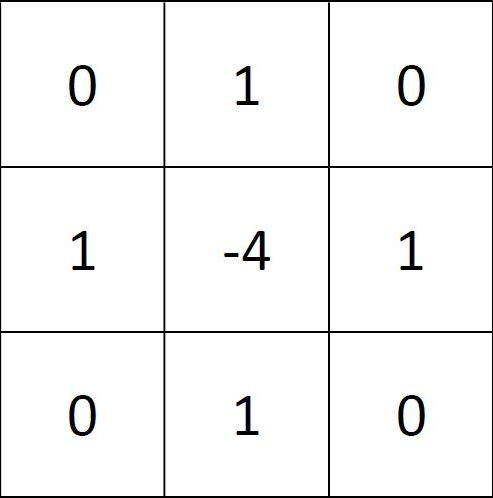
\includegraphics[width=0.2\textwidth]{Laplace-Matrix_1}}
  \qquad
  \subfloat[ ][ ]{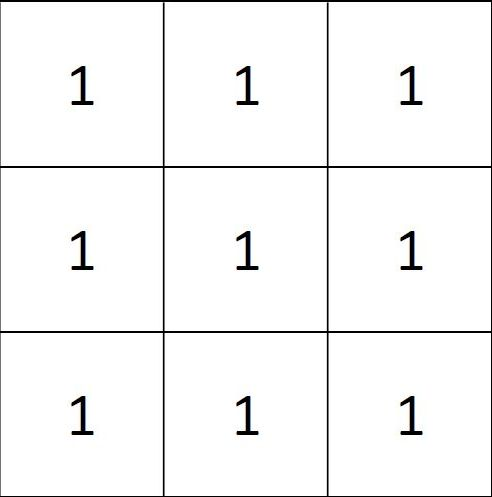
\includegraphics[width=0.2\textwidth]{Laplace-Matrix_2}}
  \caption[Laplace-Matrix]{\label{pic:Laplace-Matrix}Laplace-Matrix (a) und Pixelwerte für f(x,y) und dessen Nachbarpixel (b)}
\end{figure}

Wird beispielsweise die Laplace-Matrix aus \autoref{pic:Laplace-Matrix} (a) mit den Pixelwerten aus \autoref{pic:Laplace-Matrix} (b) verrechnet, lautet das Ergebnis der Berechnung 0. Dieses Ergebnis weist darauf hin, dass sich das mittlere Pixel in seiner Intensität nicht von seinen Nachbarpixel, die in der Berechnung berücksichtigt werden, unterscheidet.
\clearpage
%Digitale Bildverarbeitung Ende





%FPGA-Board und Hardwarebeschreibung Anfang
\section{Hardwareboard und Hardwarebeschreibung}
\label{sec:FPGA-Board und Hardwarebeschreibung}
Die in Kapitel \ref{sec:Digitale Bildverarbeitung} beschriebene digitale Bilddatenverarbeitung findet in dieser Studienarbeit in einem FPGA-Board statt. In diesem Kapitel wird erläutert, was ein FPGA-Board und dessen wichtigste Komponente, das FPGA, ist. Des Weiteren wird auf die Software \textit{Quartus Prime 18.1 Lite} eingegangen, mit der das FPGA-Board programmiert wird. Zudem wird die Hardwarebeschreibungssprache VHDL erläutert, mit der Funktionsblöcke im Programm erstellt werden können.  

\subsection{FPGA-Board} 
\label{sec:FPGA-Board}
Ein Field Programmable Gate Array (FPGA)-Board, ist ein Hardware-Board, das als Basis ein FPGA besitzt, in dem die Verarbeitung der Daten stattfindet. Zudem weist es eine Vielzahl an Anschlüssen auf, um mit Peripheriegeräten kommunizieren zu können, und es besitzt verschiedene Speicher zur Daten- und Programmspeicherung. Des Weiteren kann es Taster und Schalter zur Bedienung aufweisen sowie Anzeigeelemente, wie z.B. Siebensegmentanzeigen.\newline

\begin{figure} [h!tb]
	\begin{center}
	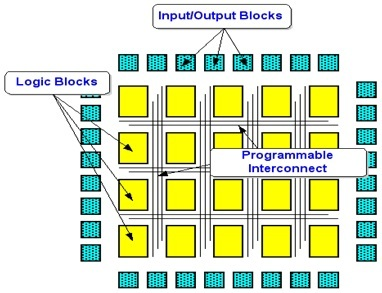
\includegraphics[width=0.5\textwidth]{FPGA-structure}
	\caption[Aufbau eines Field Programmable Gate Arrays]{\label{pic:FPGA}Aufbau eines Field Programmable Gate Arrays (FPGA) \cite{microcontrollerslab.com}}
	\end{center}
\end{figure}

Ein FPGA, das in \autoref{pic:FPGA} dargestellt ist, ist ein programmierbarer digitaler Baustein, der aus konfigurierbaren logischen Blöcken (CLBs) besteht, die in einer Matrix angeordnet sind und über programmierbare Verbindungskanäle miteinander verbunden werden können. Jeder der in \autoref{pic:CLB_PLD} a gezeigten konfigurierbaren Logikblöcke (CLBs) eines FPGAs basiert in seinem Aufbau auf einem Programmale Logic Device (PLD), das aus einer verknüpften UND-Matrix und ODER-Matrix besteht, wie es in \autoref{pic:CLB_PLD} b gezeigt ist. Durch das Aufstellen von Wahrheitstafeln, die in Look Up Tables (LUT)  gespeichert werden, wird die logische Funktion eines PLDs beschrieben. Anhand dieser Wahrheitstafel kann nun eine Programmiertabelle erstellt werden, mit deren Hilfe die UND- und ODER-Matrix programmiert wird. Die Verbindung der Eingänge und der Ausgänge eines PLDs an ein anderes erfolgt über die Programmierung der Verbindungskanäle, wobei der Ausgang eines PLDs entweder direkt angebunden oder zusätzlich über ein Flip-Flop geführt werden kann. Die Vielzahl an CLBs in einem FPGA ermöglicht es, große und komplexe Funktionen in dieses zu implementieren \cite{Tietze}.\newline %Tietze 9.1.1 / 9.1.?

\begin{figure}[h!tb]
  \centering
  \subfloat[ ][ ]{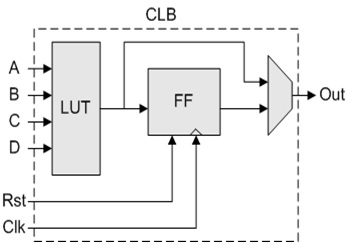
\includegraphics[width=0.3\textwidth]{FPGA-configuration-logic-blocks}}
  \qquad
  \subfloat[ ][ ]{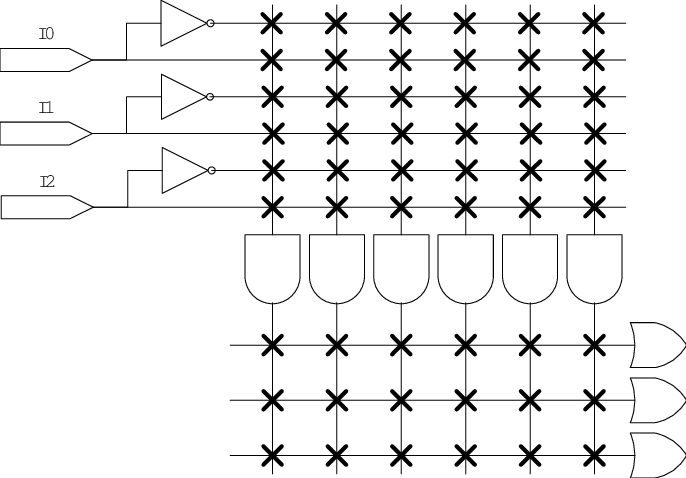
\includegraphics[width=0.3\textwidth]{Programmable-Logic-Array-PLA}}
  \caption[Aufbau eines konfigurierbaren Logikbausteins und eines Programmable Logic Device ]{\label{pic:CLB_PLD}Aufbau eines konfigurierbaren Logikbausteins (CLB) \cite{microcontrollerslab.com} (a) und Aufbau eines Programmable Logic Device (PLD) aus programmierbarer UND- und ODER-Matrix \cite{Upegui}(b)}
\end{figure}

Auf einem FPGA-Board befinden sich neben dem FPGA auch noch weitere Bauteile wie i.d.R ein Random Acces Memory (RAM) zur Datenspeicherung und ein Flash-Speicher zur Programmspeicherung. Zudem hat es Input/Output (I/O)-Anschlüsse, um Daten mit Peripheriegeräten auszutauschen bzw. von diesen Daten zu empfangen, zu verarbeiten und wieder an ein Peripheriegerät auszugeben. Die I/O-Anschlüsse können z.B. ein Video Graphics Array (VGA)-Anschluss, um Bilder an einem Monitor darzustellen, ein USB-Anschluss, ein  RS232-Anschluss oder eine Ethernetverbindung sein \cite{Tietze}.\newline %Tietze 9.1.2.1 Typenübersicht

Die Programmierung der Funktion eines FPGAs erfolgt über die Beschreibung des Schaltungsverhaltens der Hardware mittels einer Software, wie z.B. Quartus Prime 18.1 Lite(Kapitel \ref{sec:Quartus Prime 18.1 Lite}). Dieses Schaltungsverhalten wird mittels Logikplänen und Hardwarebeschreibungssprachen, wie z.B. VHDL (Kapitel \ref {sec:VHDL}), beschrieben. Über eine Schaltplaneingabe im Logikplan können Verbindungen zwischen einzelnen Teilfunktionen, die mit VHDL beschrieben wurden, und schon in Bibliotheken hinterlegten Funktionen, wie Addierer, Multiplexer und Demultiplexer, gezogen werden. Sind alle Eingaben getätigt, werden alle Verbindungen und VHDL-Beschreibungen in logische Funktionen überführt, auf ihre Syntax überprüft und gegebenenfalls von einem Simplifier vereinfacht. Danach wird das Programm auf das FPGA übertragen, wobei durch einen \textit{Device-Fitter} noch Anpassungen an die spezifische Architektur des FPGAs durchgeführt werden, damit die verfügbaren Ressourcen optimal genutzt werden \cite{Tietze}. %Tietze 9.1.3 Computer-gestützerter PLD-Entwurf



\subsection{Quartus Prime 18.1 Lite}
\label{sec:Quartus Prime 18.1 Lite}
Die Software \textit{Quartus Prime 18.1 Lite} ist eine FPGA-Design Software der Firma Intel Corporation. Die Hardwarebeschreibung eines FPGAs kann mittels einer Schematic, dies ist ein Schalt- bzw. Logikplan, und den Hardwarebeschreibungssprachen VHDL (Kapitel \ref {sec:VHDL}) und Verilog erfolgen.\newline

Mit dieser Software ist es möglich, Projekte zu erstellen, um Hardwarebeschreibungen für FPGAs durchzuführen. Nach der Erstellung des Projektes wird in der Schematic die Schaltung bzw. der Logikplan der Hardware erstellt. Dazu werden die benötigten Ein- und Ausgänge, logischen Blöcke, arithmetischen Blöcke und selbsterstellte Funktionsblöcke, die mithilfe von VHDL oder Verilog geschrieben werden können, platziert und verbunden. Mittels des integrierten Compilers wird das Hardwaredesign synthetisiert, platziert, gerootet und anschließend eine Geräteprogrammierungsdatei, ein SRAM Object File (.sof), erstellt. Mithilfe des Programmers wird die erstellte Geräteprogrammierungsdatei genutzt, um das FPGA über den JTAG-Modus zu konfigurieren und die erstellte Funktion auf das Board zu übertragen. Da dies lediglich eine flüchtige Programmierung des FPGAs ist, die bei Verlust der Spannungsversorgung verloren geht, kann über einen Programmer Object File (.pof) eine dauerhafte Speicherung erfolgen. Die .pof-Datei kann über eine Konvertierung der .sof-Datei erstellt werden und mittels des Programmers im Active Serial (AS) Programming Mode auf ein serial configuration device mit Flashspeicher im FPGA-Board geladen werden. Aus diesem wird bei erneuter Spannungsversorgung das Programm in das FPGA geladen \cite{Intel}.%Website Intel Quartus Prime https://www.intel.com/content/www/us/en/programmable/products/design-software/fpga-design/quartus-prime/user-guides.html



\subsection{VHDL} %Bild für entity und architectur einfügen
\label{sec:VHDL}
Die \textit{Very High Speed Integrated Circuit Hardware Description Language} (VHDL) ist eine Hardwarebeschreibungssprache, mit der digitale, logische Schaltungen entworfen werden. Mittels Konstrukten und Befehlen werden Abläufe und das zeitliche Verhalten von Schaltungen in einem FPGA oder Application Specific Integrated Circuit (ASCI) beschrieben. Diese Konstrukte umfassen Logikkonstrukte wie z.B. UND-, Oder- und NAND-Schaltungen, Bedingungs- und Schleifenkonstrukte wie z.B. if-Anweisungen oder for-Schleifen sowie mathematische Formeln. Die Befehle dienen dazu Funktionen und Teilschaltungen in Module zusammenzufassen, wodurch Hierarchien aufgebaut werden können {\cite{VHDL-mikrocontroller}.\newline

Eine Hardwarebeschreibung mittels VHDL basiert auf einer bestimmten Syntaxnotation. Zuerst wird eine \textit{entity} erstellt, die die Schnittstellenbeschreibung des VHDL-Funktionsblocks nach außen darstellt. Dort werden in der \textit{generic}-Umgebung Parameter deklariert, wenn diese benötigt werden. Im Abschnitt \textit{port} werden die Ein- und Ausgangssignale des Funktionsblocks beschrieben, die die Kommunikation nach außen, also die Schnittstellenbeschreibung, festlegen. Nach der \textit{entity} erfolgt das Erstellen der \textit{architecture}, die die Funktionalität des VHDL-Funktionsblocks beschreibt. Dies umfasst die Deklaration von lokalen Signalen, die nur in dieser \textit{architecture} benötigt werden, um zwischen Funktionselementen und Blöcken in der \textit{architecture} Informationen auszutauschen sowie die VHDL-Anweisungen, mit denen das Verhalten des Funktionsblocks beschrieben wird. Diese VHDL-Anweisungen umfassen über die im obigen Abschnitt beschriebenen Konstrukte und Befehle hinaus viele weitere \cite{Reichard VHDL}.\newline %Reichardt VHDL-Synthese 1.4 und 2.1
\clearpage
%FPGA-Board und Hardwarebeschreibung Ende
%Grundlagen Ende





%Haupteil anfang
%Aufbau und Hardwarekomponenten Anfang
\section{Aufbau und genutzte Hardwarekomponenten}
\label{sec:Aufbau und Hardwarekomponenten}
Der Aufbau mit der verwendeten Hardware ist in \autoref{pic:Aufbau} dargestellt. Dieser umfasst die Kameras \textit{STC-CMB33PCL} der Firma Semtech und das FPGA-Board \textit{DE2-115} der Firma Terasic mit der Erweiterungskarte \textit{CLR-HSMC Daughter Card} (Camera Link Receiver High Speed Mezzanine Card).
Die Kamera ist über die Kameraschnittstelle Camera Link mit der CLR-HSMC Daughter Card verbunden, die über den HSMC-Anschluss des DE2-115-Boards angeschlossen ist.

\begin{figure} [h!tb]
	\begin{center}
	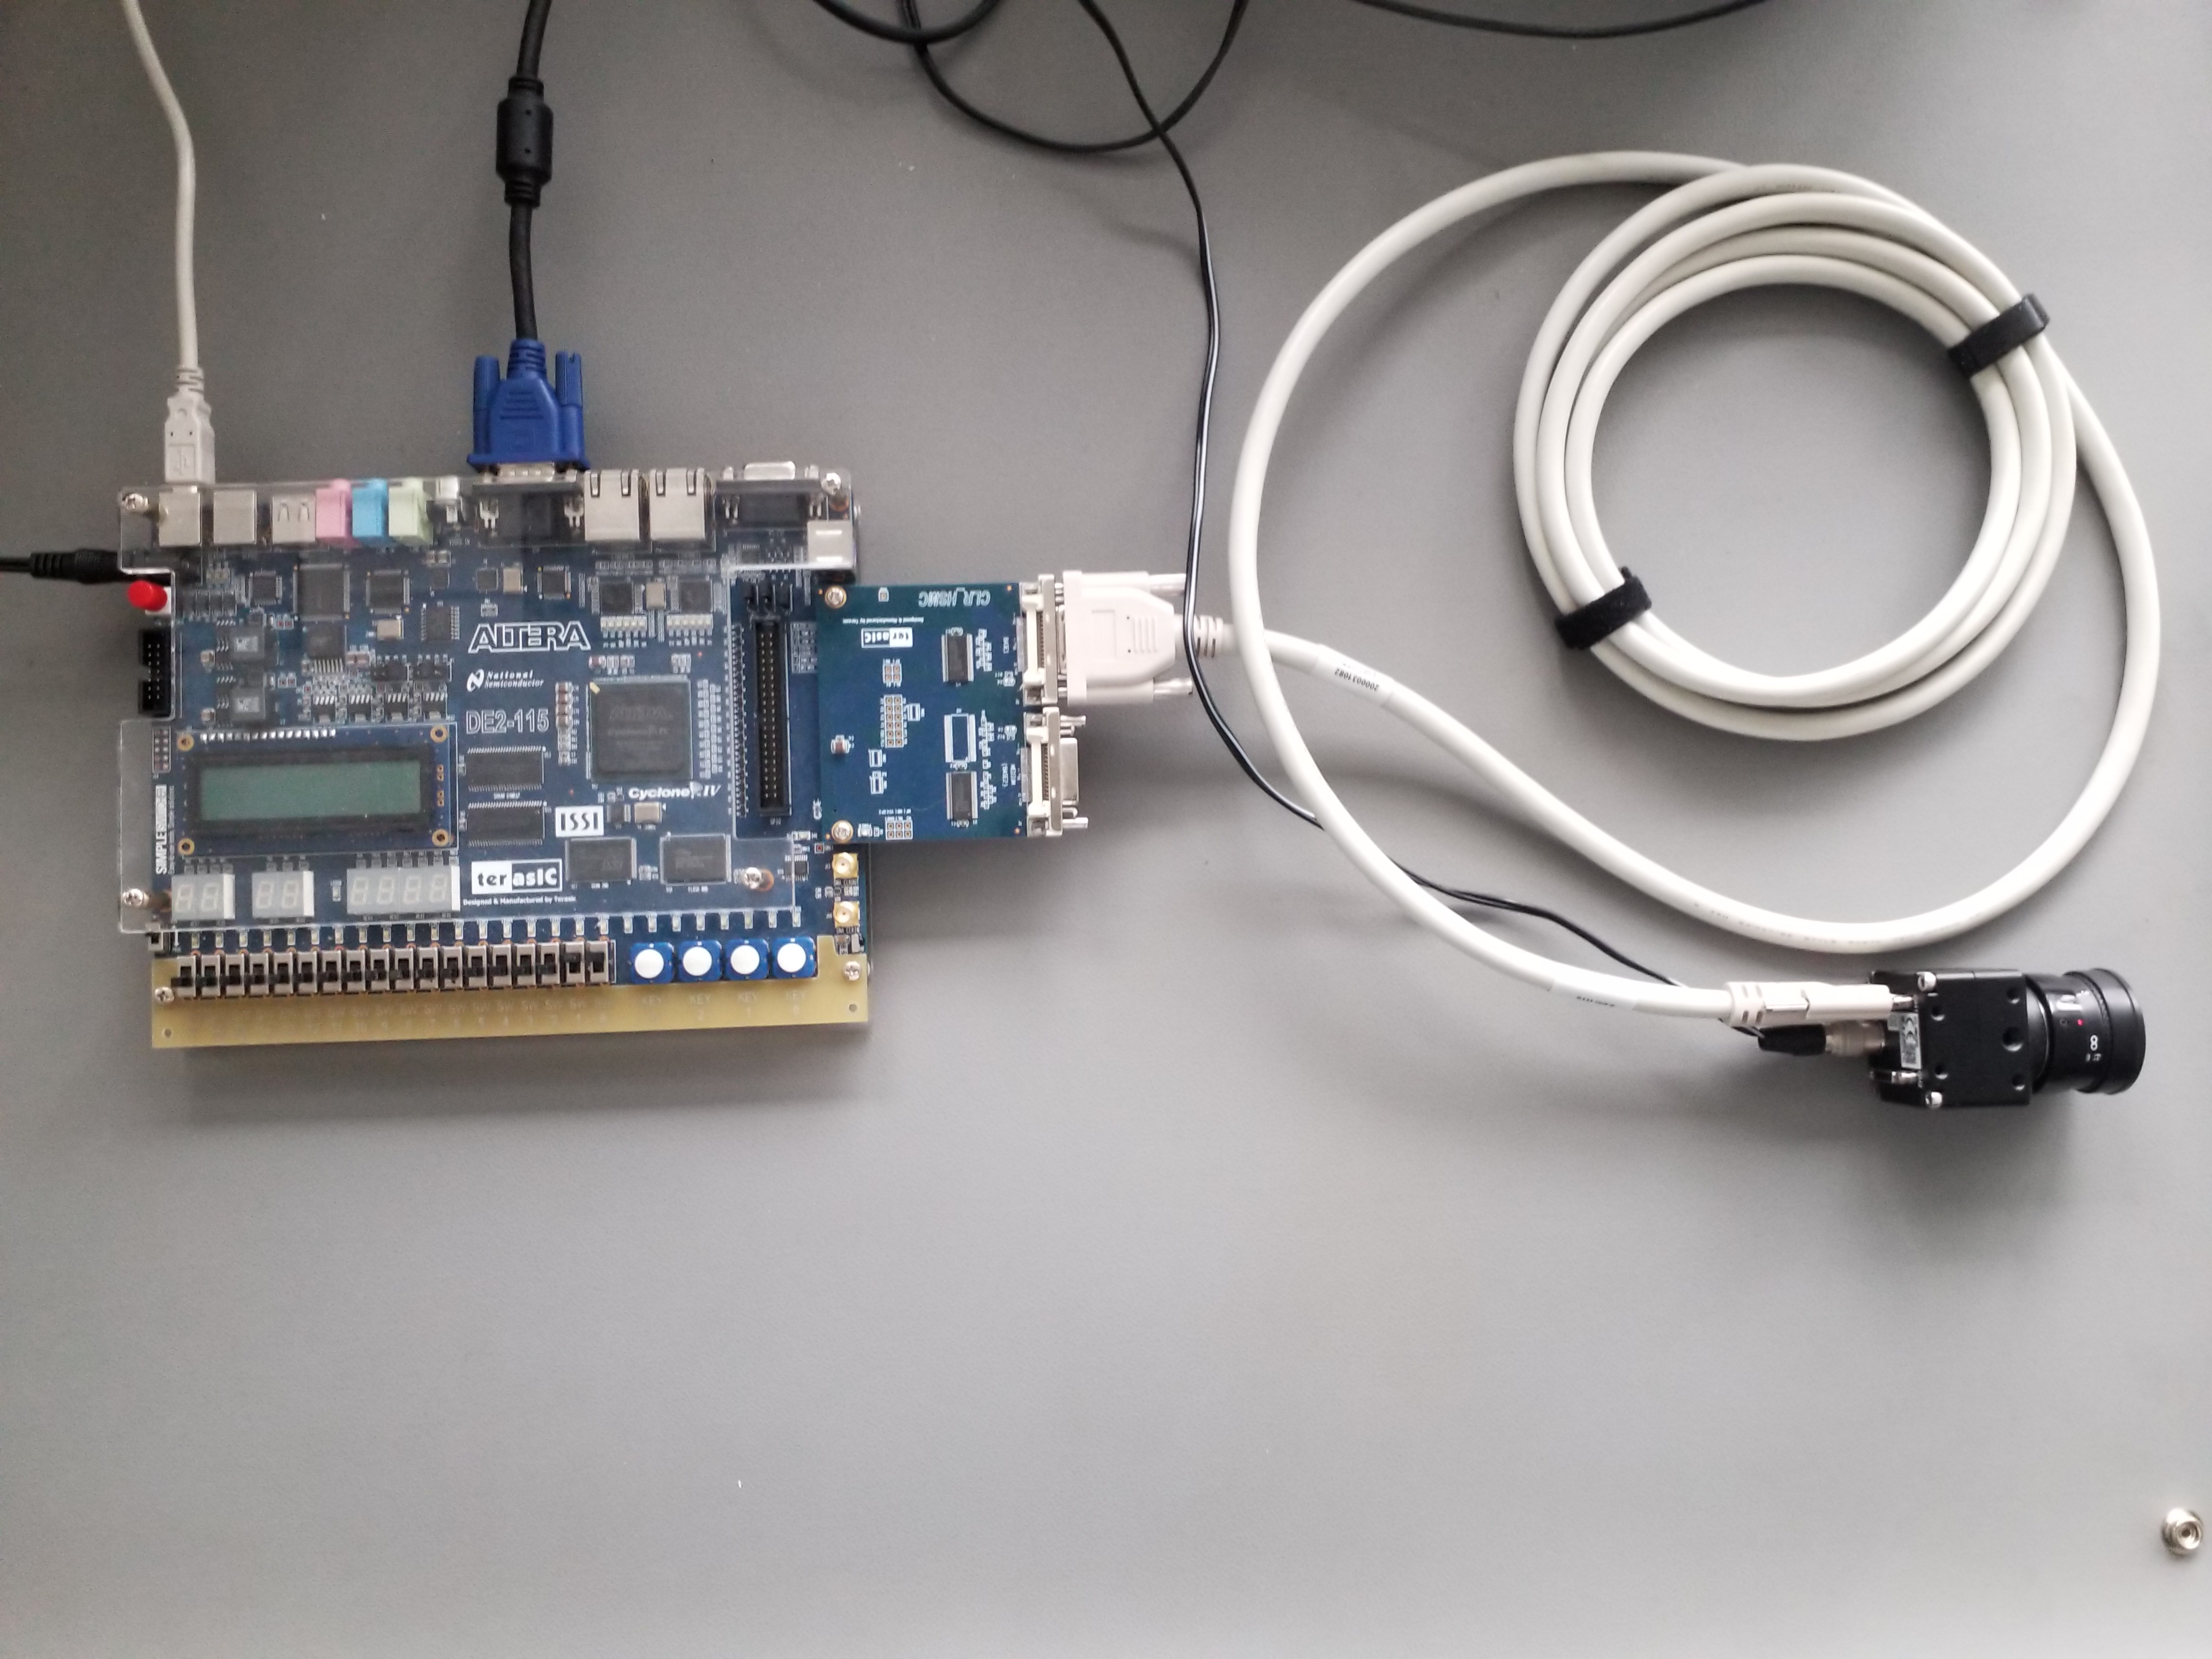
\includegraphics[width=0.5\textwidth]{Gesamter_Aufbau_1_20190930_135046}
	\caption[Aufbau mit Kamera STC-CMB33PLC und FPGA-Board DE2-115]{\label{pic:Aufbau}Aufbau mit Kamera STC-CMB33PLC und FPGA-Board DE2-115}
	\end{center}
\end{figure}



\subsection{Kamera STC-CMB33PCL}
\label{sec:Kamera STC-CMB33PCL}
In \autoref{pic:Kamera STC-CMB33PCL und Anschlüsse} ist die verwendete Kamera STC-CMB33PCL dargestellt, welche maximal 494 frames per second (FPS) aufnehmen kann. Die aufgenommenen Bilder sind monochrome Bilder, die in Graustufen dargestellt werden. Die Kamera besitzt drei Anschlüsse, einen Base Camera Link Connector, einen Medium Camera Link Connector und einen Power I/O Connector.\newline

\begin{figure}[h!tb]
  \centering
  \subfloat[ ][ ]{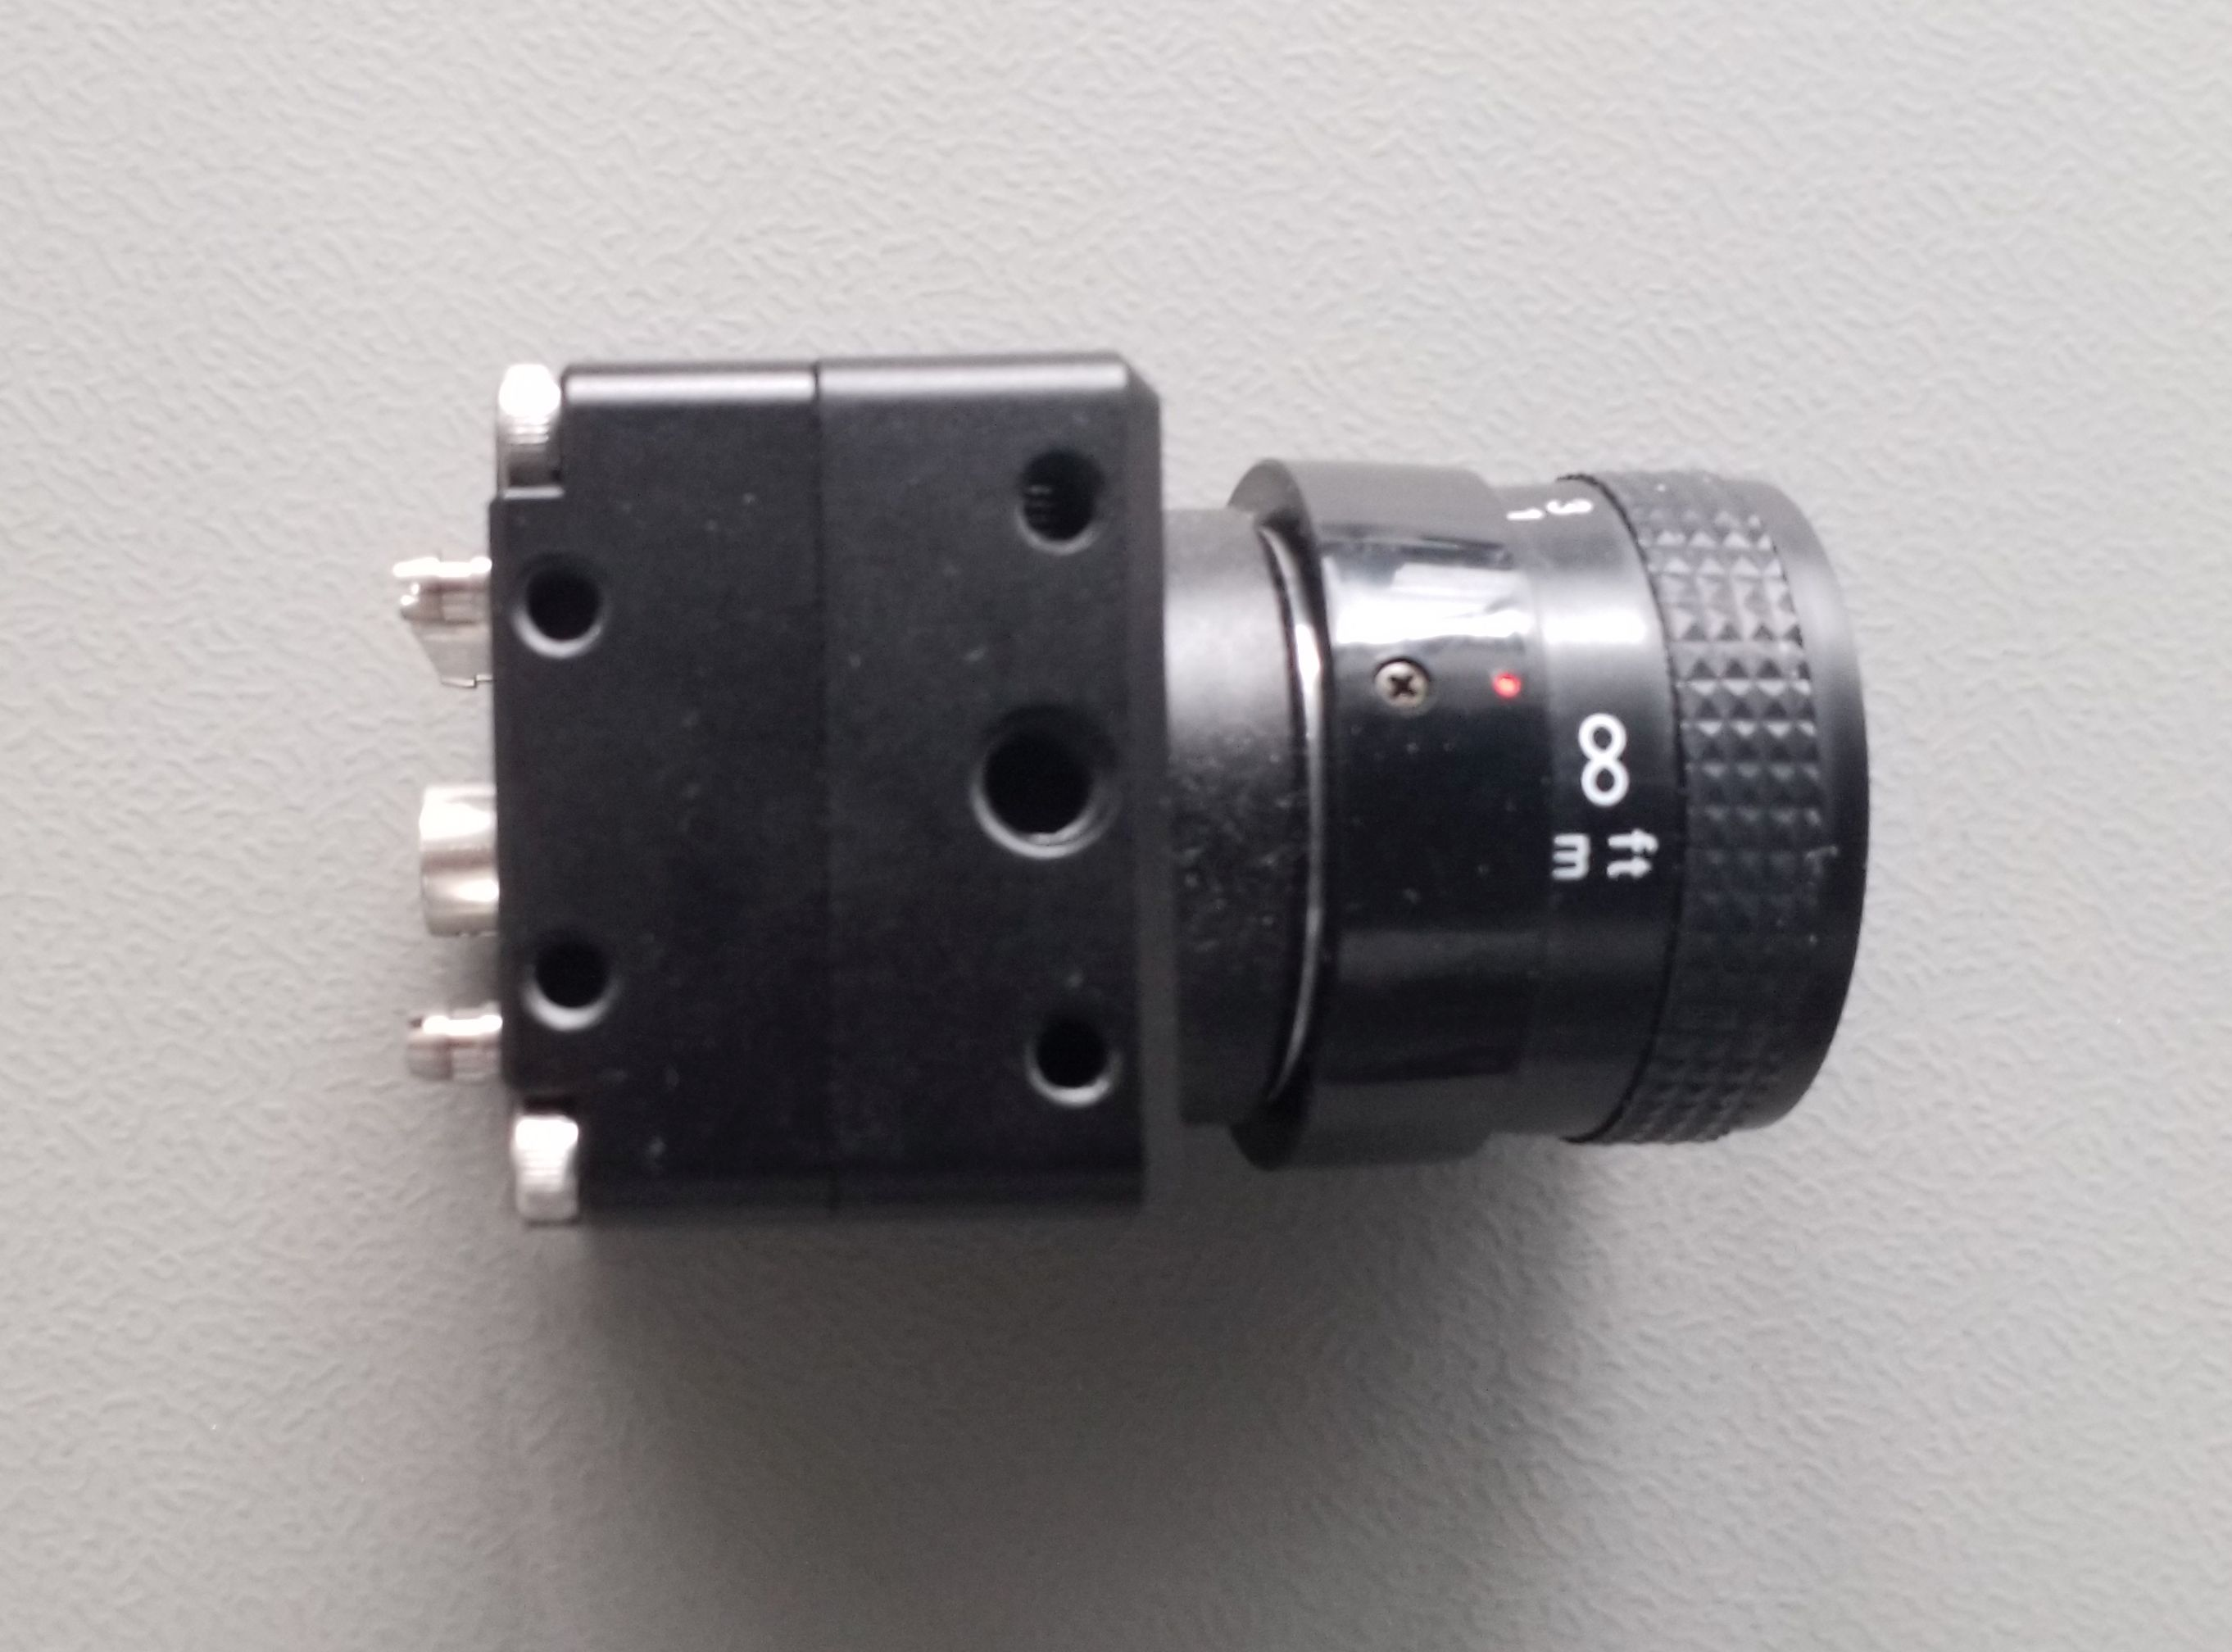
\includegraphics[width=0.25\textwidth]{Kamera_oben_2_20190930_130438_bearbeitet}}
  \qquad
  \subfloat[ ][ ]{\includegraphics[width=0.25\textwidth]{Kamera_Anschlüsse_1_20190930_130459_bearbeitet}}
  \caption[Kamera STC-CMB33PCL und Anschlüsse]{\label{pic:Kamera STC-CMB33PCL und Anschlüsse}Kamera STC-CMB33PCL(a) und Anschlüsse(b)}
\end{figure}

Über den Power I/O Connector wird die Kamera mit Spannung versorgt und über den Base Camera Link Connector (Channel 1) ist die Kamera mit der Erweiterungskarte verbunden. Diese Verbindung erfolgt über ein Camera Link Kabel, das über einen 26-Pin Shrunk Delta Ribbon (SDR)-Anschluss an die Kamera und einen Recommended Standard (RS)-232 Anschluss an die Erweiterungskarte angeschlossen ist.\\
Die verwendete Schnittstelle Camera Link ist ein Standard der Automated Imaging Association (AIA), der in der industriellen Bildverarbeitung genutzt wird und über die die Daten mehrerer Pixel gleichzeitig übertragen werden können. Sie weist die Implementierungen Base, Medium und Full auf, die verschiedene Datenübertragungsraten ermöglichen, siehe \autoref{pic:Implementierung und Aufbau von Camera Link} a \cite{Stemmer a}. So können beispielsweise bei Base 3 Pixel mit je 8 Bit oder 2 Pixel mit 10 oder 12 Bit übertragen werden. Die zu übertragenden Daten werden über einen Multiplexer geführt und dann mittels Low Voltage Differential Signaling (LVDS)-Aderpaaren auf einen Demultiplexer geführt, der die Daten wieder demultiplext und für die weitere Verarbeitung zur Verfügung stellt. Dieser Aufbau ist beispielhaft an der Base Camera Link Konfiguration in \autoref{pic:Implementierung und Aufbau von Camera Link} b dargestellt \cite{Wikipedia a}.

\begin{figure}[h!tb]
  \centering
  \subfloat[ ][ ]{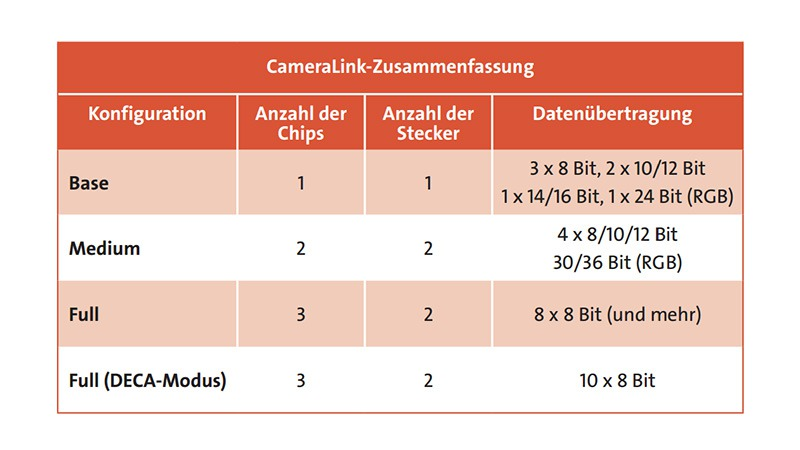
\includegraphics[width=0.7\textwidth]{stemmer_glossary-cameralink-implementierungen}}
  \qquad
  \subfloat[ ][ ]{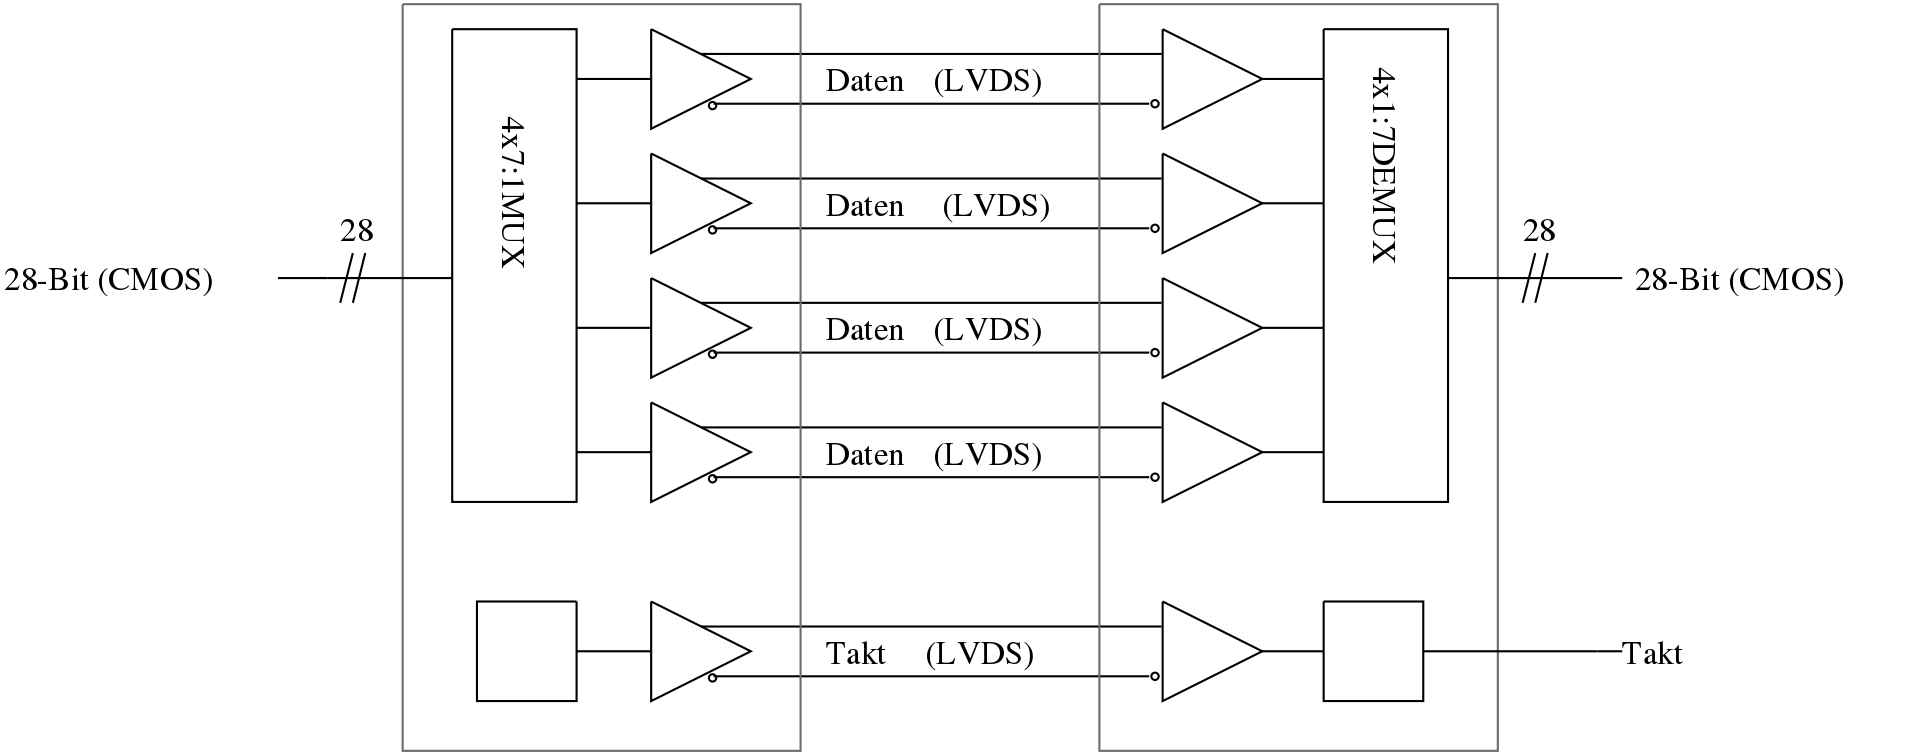
\includegraphics[width=0.7\textwidth]{wikipedia_cameralink}}
  \caption[Implementierungen und Aufbau von Camera Link ]{\label{pic:Implementierung und Aufbau von Camera Link} Implementierungen (a) \cite{Stemmer a} und Aufbau (b)  \cite{Wikipedia a} der Camera Link Schnittstelle}
\end{figure}

Die Einstellung der Kamera kann unterschiedlich mittels der Software \textit{CLCtrl2} parametriert werden. So kann über verschiedene Parameter eingestellt werden, wie viele Zeilen und Spalten ein Bild hat, ob mehrere kleine Teilbilder aus dem Kamerabild übertragen werden sollen und ob die Daten für 2 oder 3 Pixel mit je 8, 10 oder 12 Bit ausgegeben werden. Die Parameter werden so eingestellt, dass ein Kamerabild 484 Zeilen und 642 Spalten hat und dass je 2 Pixel, die je 8 Bit lang sind, pro Takt ausgegeben werden, entsprechend der Übertragung der Daten über den Base Camera Link Connector der Kamera. Zudem werden der Zustand der Signale  LVAL, FVAL, DVAL und die Pixelfrequenz, mit der die Ausgabe der Pixel stattfindet, übertragen. Diese hat bei den eingestellten Parametern eine Frequenz von 84 MHz \cite{Sentech}.\newline

\begin{figure} [h!tb]
	\begin{center}
	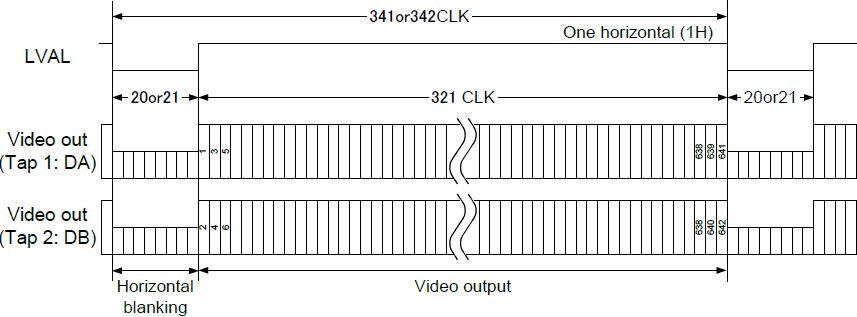
\includegraphics[width=0.7\textwidth]{LVAL_neu}
	\caption[Horizontales Timing mit dem Signal LVAL]{\label{pic:LVAL}Horizontales Timing mit dem Signal LVAL \cite{Sentech}}
	\end{center}
\end{figure}

Die \autoref{pic:LVAL} zeigt die Funktion des Signals LVAL. Dieses signalisiert, ob die Kamera gerade Daten für die Pixel einer Zeile ausgibt oder nicht. Das Signal ist für 321 Takte (1 Takt = 11,9 ns) auf high gesetzt. In dieser Zeit werden die Daten für die Pixel einer Zeile ausgegeben, wobei pro Takt Daten für 2 Pixel, Tap1 und Tap2, ausgegeben werden. Danach ist das Signal für 20 oder 21 Takte auf low gesetzt. Durch den Signalwechsel von low auf high wird signalisiert, dass die Ausgabe einer neuen Zeile beginnt. In der \autoref{pic:LVAL_Pixel_Order} ist zudem dargestellt, in welcher Reihenfolge die Pixel eines Bildes ausgegeben werden. Es werden immer die Pixel einer Zeile von links nach rechts und die Zeilen von oben nach unten ausgegeben. Das Signal DVAL besitzt die gleiche Funktion wie das Signal LVAL \cite{Sentech}.\newline

\begin{figure} [h!tb]
	\begin{center}
	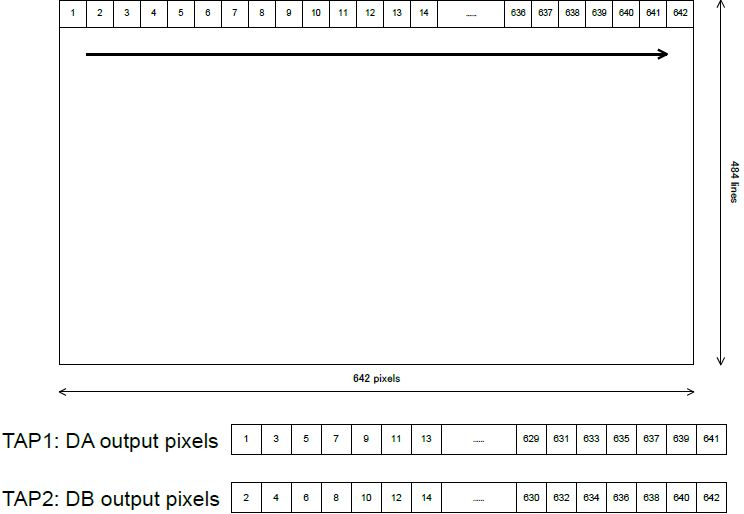
\includegraphics[width=0.7\textwidth]{LVAL_Pixel_Order_neu}
	\caption[Reihenfolge der Übertragung der einzelnen Pixel für ein Bild]{\label{pic:LVAL_Pixel_Order}Reihenfolge der Übertragung der einzelnen Pixel für ein Bild \cite{Sentech}}
	\end{center}
\end{figure}

Die Funktion des Signals FVAL ist in \autoref{pic:FVAL} dargestellt. Das Signal ist high, solange die 484 Zeilen eines Bildes ausgegeben werden. Nach der Ausgabe der 484 Zeilen wechselt das Signal von high auf low. In diesem Zustand verbleibt es für 14 Takte und durch den Wechsel von low auf high wird signalisiert, dass die Ausgabe der Pixeldaten eines neuen Bildes beginnt \cite{Sentech}.\newline

\begin{figure} [h!tb]
	\begin{center}
	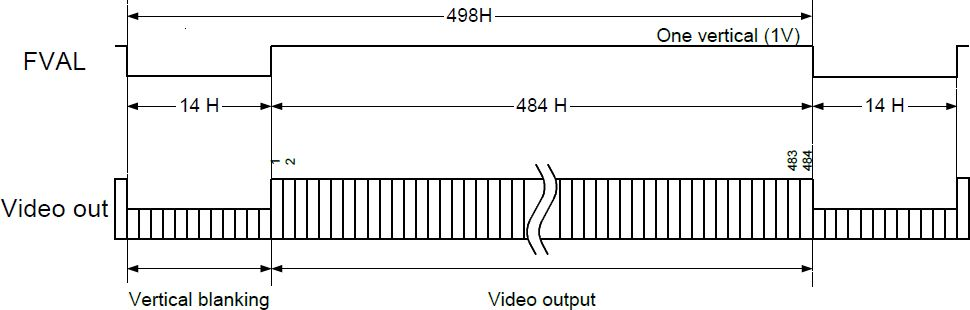
\includegraphics[width=0.7\textwidth]{FVAL_neu}
	\caption[ertikales Timing mit dem Signal FVAL]{\label{pic:FVAL}Vertikales Timing mit dem Signal FVAL (Quelle: \cite{Sentech})}
	\end{center}
\end{figure}

Die Kamera STC-CMB33PCL der Firma Semtech stand ebenfalls zur Verfügung, wurde aber nicht genutzt, da diese Kamera Farbbilder liefert und daher nicht benötigt wurde, weil sich die Studienarbeit zuerst mit der Verarbeitung von Schwarzweißbildern beschäftigt.\newline



\subsection{FPGA-Board Altera DE2-115}
\label{sec:FPGA-Board Altera DE2-115}
Die Verarbeitung der Kameradaten findet in dem in \autoref{pic:DE2-115} dargestellten FPGA-Board DE2-115 der Firma Terasic statt. Als FPGA zur Datenverarbeitung dient ein \textit{Altera Cyclone IV EP4CE115} mit 114.480 Logikeinheiten, 432 M9K-Speicherblöcken, 3.888 Kbit eingebettetem Speicher und 4 Phase Locked Loop (PLL).\newline

\begin{figure} [h!tb]%Bildquelle DE2-115 User Manuel Figure 2-1 The DE2-115 board (top view)
	\begin{center}
	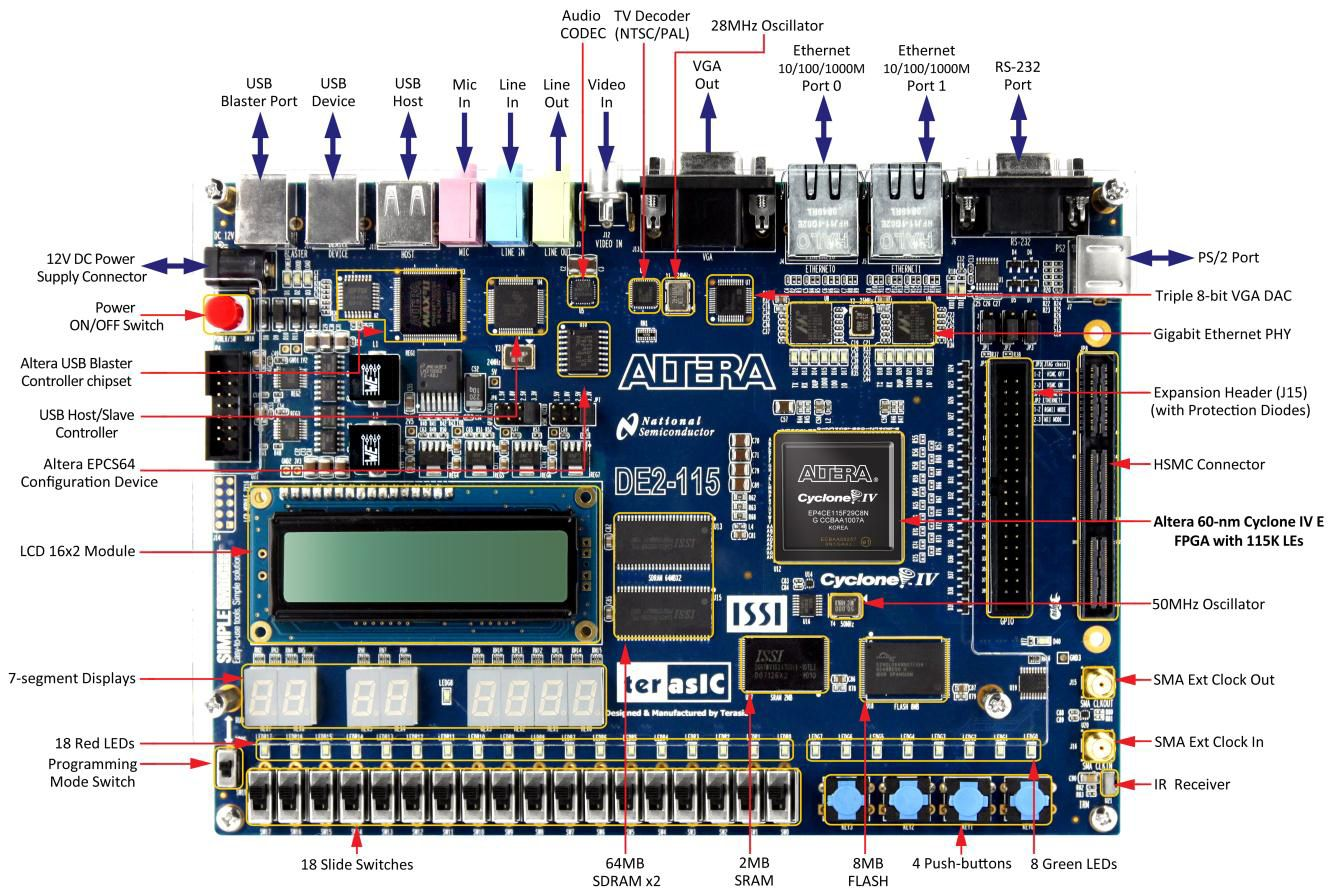
\includegraphics[width=0.75\textwidth]{DE2-115}
	\caption[FPGA-Board Altera DE2-115]{\label{pic:DE2-115}DE2-115  (Quelle: \cite{Terasic b})}
	\end{center}
\end{figure}

Das Board hat diverse Anschlüsse wie z.B. einen USB-Anschluss, einen VGA-Anschluss und einen RS232-Anschluss, um Daten an Peripheriegeräte ausgeben oder von diesen erhalten zu können. Zudem hat es einen 2MB SRAM, zwei 64MB SDRAMs und einen 8MB Flash Speicher. Des Weiteren hat das DE2-115 Board 18 Schalter und 4 low-aktive Taster und als Anzeigeelemente besitzt es ein LCD 16x2 Modul, acht Siebensegment-Anzeigen, 18 rote LEDs und neun grüne LEDs. Zur Generierung von Taktsignalen fungieren drei 50MHz Oszillatoren. Das Blockdiagramm des DE2-115 ist in \autoref{pic:DE2-115 Blockdiagramm} dargestellt, welches die internen Verbindungen der einzelnen Komponenten des DE2-115 zeigt \cite{Terasic b}.%DE2-115 User Manuel 2.1 Layout und Components

\begin{figure} [h!tb]%Bildquelle DE2-115 User Manuel Figure 2-3 Block Diagram of DE2-115
	\begin{center}
	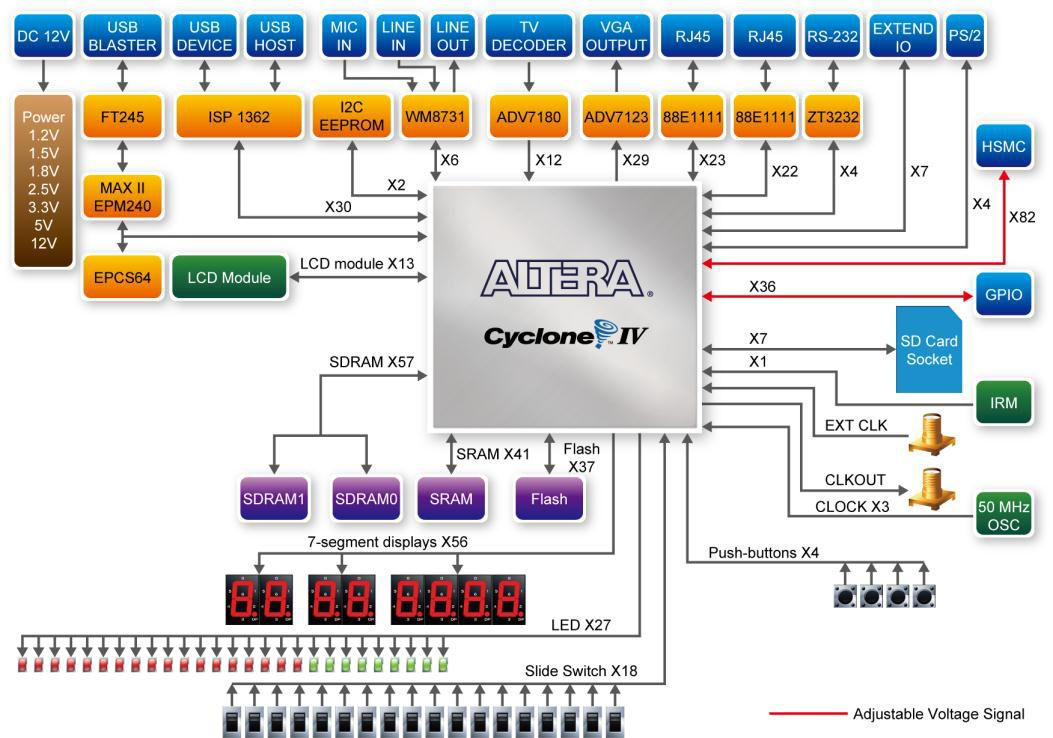
\includegraphics[width=0.75\textwidth]{DE2-115 Blockdiagramm}
	\caption[DE2-115 Blockdiagramm]{\label{pic:DE2-115 Blockdiagramm}DE2-115 Blockdiagramm (Quelle: \cite{Terasic b})}
	\end{center}
\end{figure}

Über den HSMC-Anschluss ist die in \autoref{pic:CLR-HSMC Board} dargestellte Erweiterungskarte CLR-HSMC Daughter Card an das FPGA-Board angeschlossen. Diese Erweiterungskarte wird benötigt, um die Bilddaten über die Camera Link Schnittstelle der Kamera auf das FPGA-Board zu übertragen, da das FPGA-Board keine eigene Camera Link Schnittstelle hat. 

\begin{figure} [h!tb]%Bildquelle CLR-HSMC User Guide Figure 2.1
	\begin{center}
	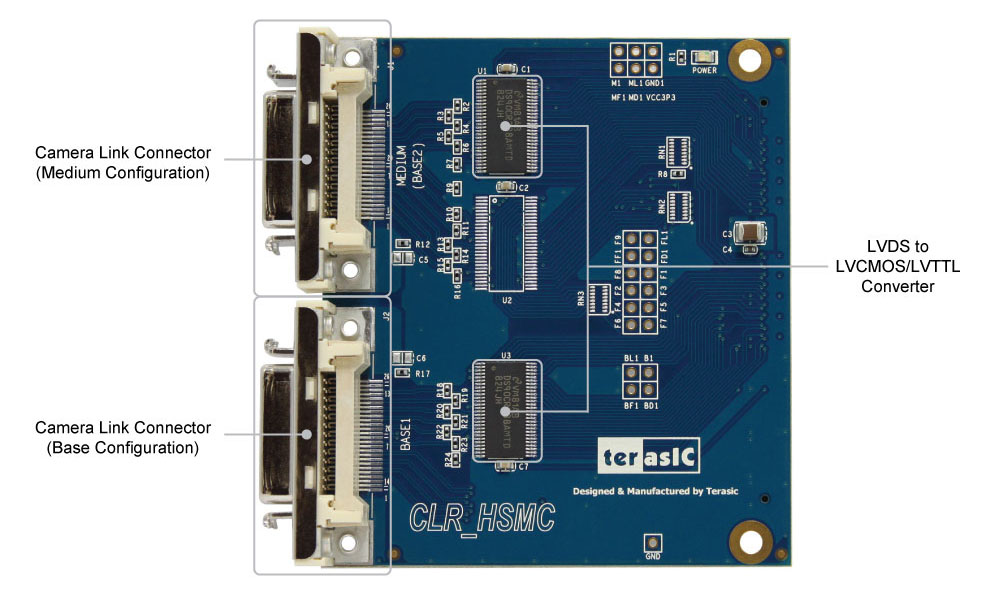
\includegraphics[width=0.5\textwidth]{CLR_HSMC_Oberseite}
	\caption[CLR-HSMC Board]{\label{pic:CLR-HSMC Board}CLR-HSMC Board (Quelle: \cite{Terasic b})}
	\end{center}
\end{figure}

Die Konfigurierung des FPGAs und damit die Verarbeitungsweise der Bilddaten erfolgt über den USB-Blaster-Anschluss, indem die mit der Software \textit{Quartus Prime 18.1 Lite} erstellte Konfigurationsdatei mittels des Programmers dieser Software auf das FPGA-Board übertragen werden, wie es in Kapitel \ref{sec:Quartus Prime 18.1 Lite} beschrieben ist. Wenn die .sof-Datei im JTAG-Mode in das FPGA geladen werden soll, muss der Programming Mode Switch des FPGA-Board in die RUN-Stellung gebracht werden. Wird die .pof-Datei im AS-Mode in das serial configuration device EPCS64 geladen, um das Programm dauerhaft zu speichern, muss der Programming Mode Switch auf PROG gestellt werden\cite{Terasic b}.
\clearpage
%Aufbau und Hardwarekomponenten Ende





%Stand zu Bearbeitungsbeginn Anfang
\section{Aktueller Stand}
\label{sec:Stand zu Bearbeitungsbeginn}
Zu Beginn der Studienarbeit war es möglich, das Kamerabild im FPGA zwischenzuspeichern und über den VGA-Anschluss an einen Monitor auszugeben. Dazu wurden mehrere Funktionsblöcke mittles VHDL in der Software \textit{Quartus Prime 18.1 Lite} geschrieben und mit weiteren Funktionsblöcken verknüpft, die in \autoref{pic:Ablauf der Bilddatenverarbeitung und Funktionsblock altll0} a dargestellt sind. Dabei wurden die Bausteine cameralink\_tapping\_base, camera\_data\_mux\_gen, MemoryAccessContoller, SDRAM\_Write\_Buffer\_gen und SDRAM\_Read\_Buffer\_gen entworfen. Der Funktionsblock vga\_controller ist ein fertiger Baustein von Scott Larson \cite{Digi-Key}. Der dram sowie der sdram\_controller\_latency1 sind Funktionsblöcke der Firma Altera Cooperation. Zusätzlich zu diesen Funktionsblöcken erzeugt der Funktionsblock altll0 (\autoref{pic:Ablauf der Bilddatenverarbeitung und Funktionsblock altll0} b), der ebenfalls von der Altera Cooperation stammt, die drei Taktsignal vga\_pixel\_clk mit 25 MHz, clk\_pll mit 100 MHz und DRAM\_CLK\_TEST mit 100MHz und $-60^\circ$ Phasenverschiebung, mit denen ein Teil der anderen Funktionsblöcke arbeitet. Zudem gibt es den Funktionsblock seg7dec, der die Ansteuerung der Elemente der Siebensegmentanzeige übernimmt (\autoref{pic:Ablauf der Bilddatenverarbeitung und Funktionsblock altll0} c).

\begin{figure}[h!tb]
  \centering
  \subfloat[ ][ ]{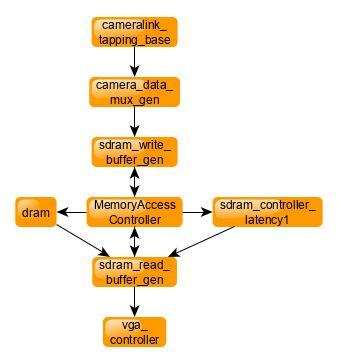
\includegraphics[width=0.4\textwidth]{Blockschaltbild_Quartus_Ist_Stand_vor_beginn_neu_191209}}
  \qquad
  \subfloat[ ][ ]{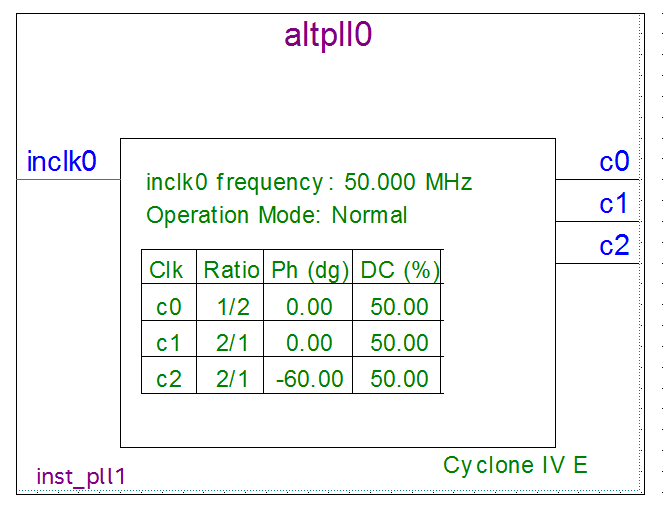
\includegraphics[width=0.4\textwidth]{altpll0}}
  \qquad
  \subfloat[ ][ ]{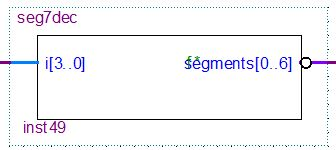
\includegraphics[width=0.3\textwidth]{7_Segmentanzeige_bearbeitet}}
  \caption[Ablauf der Bilddatenverarbeitung und Funktionsblöcke altll0 und seg7dec]{\label{pic:Ablauf der Bilddatenverarbeitung und Funktionsblock altll0}Ablauf der Bilddatenverarbeitung vor Beginn der Studienarbeit (a), Funktionsblock altll0 zur Generierung der benötigten Taktsignale und Funktionsblock seg7dec zur Ansteuerung der Siebensegmentanzeigen (c)}
\end{figure}



\subsection{cameralink\_tapping\_base}
\label{sec:cameralink_tapping_base}
Über den in \autoref{pic:cameralink_tapping_base} a abgebildeten Funktionsblock \textit{cameralink\_tapping\_base} werden die Daten, die von der Kamera kommen und an der Eingangsschnittstelle TX\_RX des Funktionsblocks angelegt werden, sortiert. Dies ist notwendig, da die Daten durch die Übertragung von der Kamera über die Schnittstelle Camera Link zum CLR\_HSMC-Board und anschließend zum FPGA-Board DE2-115 nicht in der richtigen Reihenfolge ankommen. So liegen z.B. die Daten für das erste Pixel in den Bits 0-4, 6, 26 und 5. Diese Funktion sortiert die Daten und gibt diese an seinen Ausgangsschnittstellen aus. An Port A werden die Daten für das erste Pixel ausgegeben, an Port B die für das zweite Pixel und an Port C die Daten für das dritte. Das Ausgangssignal LVAL gibt an, ob die Daten für eine Bildzeile gerade übertragen werden und das Ausgangssignal FVAL, ob momentan ein Bild übertragen wird.\\
Über die in \autoref{pic:cameralink_tapping_base} b dargestellten Parameter NUM\_TAPS und NUM\_BITS wird eingestellt, wie viele Pixel mit welcher Bitanzahl pro Takt von der Kamera empfangen und anschließend verarbeitet werden, wobei die Anzahl der Pixel und Bits mit dem eingestellten Werten der Kamera, die in Kapitel \ref{sec:Kamera STC-CMB33PCL} \nameref{sec:Kamera STC-CMB33PCL} beschrieben sind, übereinstimmen müssen (zwei Pixel je acht Bit).\newline 

\begin{figure}[h!tb]
  \centering
  \subfloat[ ][ ]{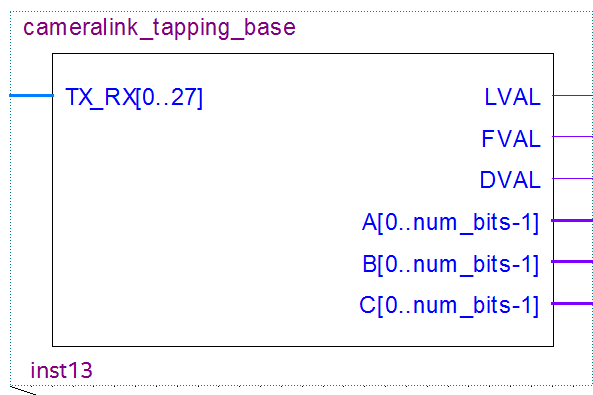
\includegraphics[width=0.4\textwidth]{cameralink_tapping_base}}
  \qquad
  \subfloat[ ][ ]{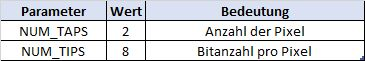
\includegraphics[width=0.4\textwidth]{Parameter_cameralink_tapping_base}}
  \caption[Funktionsblock cameralink\_tapping\_base mit Parameterbeschreibung]{\label{pic:cameralink_tapping_base}Funktionsblock cameralink\_tapping\_base (a) mit Parameterbeschreibung (b)}
\end{figure}



\subsection{camera\_data\_mux\_gen}
\label{sec:camera_data_mux_gen}
Die von dem Funktionsblock \textit{cameralink\_tapping\_base} ausgegebenen Daten LVAL, FVAL, Port A und Port B werden von dem in \autoref{pic:camera_data_mux_gen} a dargestellten Funktionsblock \textit{camaera\_data\_mux\_gen} mit den in \autoref{pic:camera_data_mux_gen} b beschriebenen Parametern aufgenommen und verarbeitet.\newline

\begin{figure}[h!tb]
  \centering
  \subfloat[ ][ ]{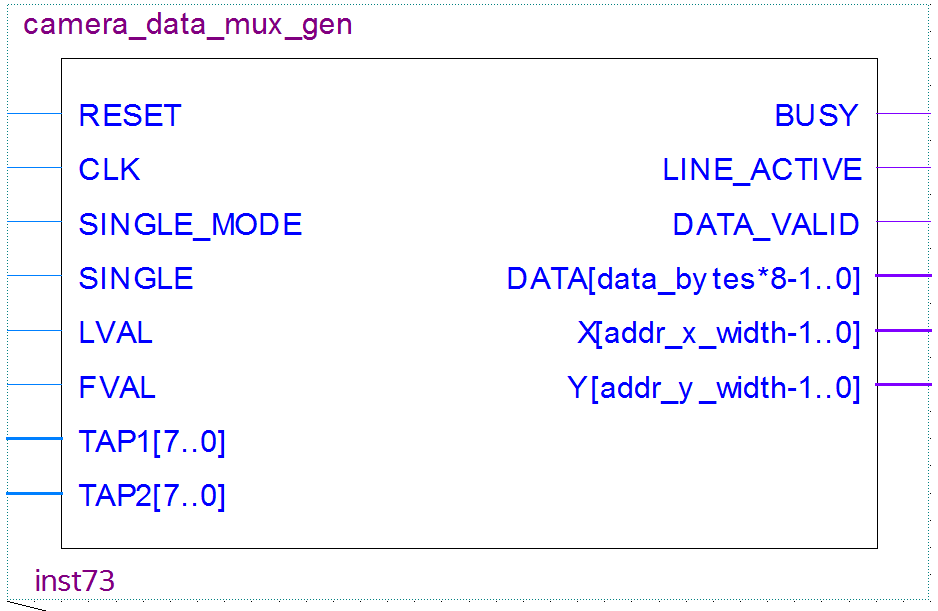
\includegraphics[width=0.4\textwidth]{camera_data_mux_gen}}
  \qquad
  \subfloat[ ][ ]{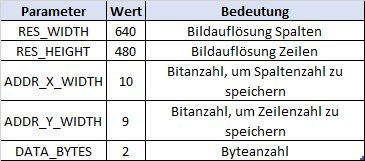
\includegraphics[width=0.4\textwidth]{Parameter_camera_data_mux_gen}}
  \caption[Funktionsblock camera\_data\_mux\_gen mit Parameterbeschreibung]{\label{pic:camera_data_mux_gen}Funktionsblock camera\_data\_mux\_gen (a) mit Parameterbeschreibung (b)}
\end{figure}

Die Daten für zwei Pixel werden an den Eingangsschnittstellen TAP1[7..0] und TAP2[7..0] aufgenommen und zusammen am Ausgang DATA wieder ausgegeben, was über eine Zustandsmaschine mit sechs Zuständen realisiert wurde. Dabei wird im Startzustand WAIT\_STATE darauf gewartet, dass ein neues Bild verarbeitet werden darf. Dies geschieht entweder dadurch, dass kontinuierlich Bilder verarbeitet werden sollen (SINGLE\_MODE = '0') oder sich ein Signalwechsel des einsynchonisierten Signals SINGLE von '1' auf '0' ereignet, der durch den Taster KEY[1] erzeugt wird, wenn SINGLE\_MODE auf '1' steht. Dadurch wird das Ausgangssignal BUSY auf '1' gesetzt, welches zeigt, dass der Funktionsblock beschäftigt ist, und es wird in den nächsten Zustand WAITFRAME\_STATE gewechselt. In diesem Zustand wird gewartet, bis ein Signalwechsel von '0' auf '1' des Signals FVAL erfolgt, das anzeigt, dass ein neues Bild übertragen wird. Es wird in den Zustand WAITLINE\_STATE gewechselt, in dem verharrt wird, bis die Übertragung der Daten einer neuen Zeile erfolgt. Dies wird durch den Signalwechsel von '0' auf '1' des Signals LVAL angezeigt. Dann werden die Daten der Eingänge TAP1 und TAP2  auf den Ausgang DATA gelegt und das Ausgangssignal DATA\_VALID auf '1' gesetzt, welches anzeigt, dass die Daten des Signals DATA gültig sind und verarbeitet werden dürfen. Zudem wird das Signal LINE\_ACTIVE auf '1' gesetzt, welches signalisiert, dass die Pixeldaten einer Bildzeile ausgegeben werden. Es erfolgt der Wechsel in den Zustand DATA\_OUT\_16BIT. In diesem Zustand wird verblieben, bis alle Pixeldaten der Bildzeile über DATA ausgegeben wurden. Danach wird entweder in den Zustand WAITLINE\_STATE gewechselt, wenn noch nicht alle Zeilen eines Bildes ausgegeben wurden, oder in den Zustand WAIT\_STATE, wenn ein Bild komplett ausgegeben wurde. Die Größe des Bildes wird über die Parameter RES\_WIDTH und RES\_HEIGHT festgelegt, wobei diese auch auf einen kleineren Wert eingestellt werden können als auf die Größe des Bildes, welches die Kamera liefert. Die überschüssigen Zeilen und Spalten gehen dann verloren. Des Weiteren gibt es noch die Zustände DATA\_OUT\_32BIT\_1 und DATA\_OUT\_32BIT\_2, die die gleiche Aufgaben wie der Zustand DATA\_OUT\_16BIT haben. Allerdings werden diese nur benötigt, wenn die Ausgabe über DATA mit 4 Bytes erfolgt anstatt mit 2 Bytes.\\
Zudem werden auf die Ausgangssignale X und Y immer die x-Koordinate des ersten Pixels und die y-Koordinate der beiden Pixel, die über DATA ausgegeben werden, gelegt. Der Funktionsblock arbeitet mit dem an CLK anliegenden Takt CLRRXCLK\_BASE. Dieser Takt ist der 84 MHz der Kamera, mit dem die Pixel übertragen werden.



\subsection{MemoryAccessController}
\label{sec:MemoryAccessController}
Der Funktionsblock MemoryAccessController, der in \autoref{pic:Memory_Access_Controller} a dargestellt ist, regelt den Zugriff auf dem SDRAM des FPGA-Boards und nutzt das Taktsignal clk\_pll, das am Eingang clk angelegt wird. Zudem sind in \autoref{pic:Memory_Access_Controller} b die Parameter des Funktionsblockes dargestellt.\\
Funktionsblöcke, die auf den Speicher zugreifen möchten, senden dem MemoryAccessController eine Zugriffsanfrage an einen der Eingänge von req[7..0] und müssen die Anzahl an Takten warten, die über den Parameter DELAY eingestellt werden, ob nicht ein Funktionsblock mit höherer Priorität auf den SDRAM zugreifen möchte. Die Prioritäten werden über die Parameter PRIO\_0 bis PRIO\_7 vorgegeben. Zusätzlich zu den Requestsignalen muss ein Funktionsblock dem MemoryAccessController mitteilen, auf welche Speicheradresse er zugreifen möchte, indem die Speicheradresse an den entsprechenden Adresseingang adr0[24..0] - adr7[24..0] gelegt wird, und ob er vom Speicher lesen oder schreiben möchte. Für einen Lesezugriff muss das Signal rd[7..0] auf '1' und für einen Schreibzugriff muss das Signal wr[7..0] auf '1' gesetzt werden. Will ein Funktionsblock schreiben, muss dieser während des Schreibvorgangs zusätzlich auch die zu schreibenden Daten auf den entsprechenden Dateneingang dta0[31..0] - dta7[31..0] legen. Über das Signal ena[7..0] erteilt der MemoryAccessController die Zugriffsrechte und koordiniert danach den Zugriff, indem es die Schreib- oder Leseanfrage mit entsprechender Speicheradresse und gegebenenfalls die zu schreibenden Daten an den Speicher weiter gibt. Dies geschieht über die Signale mem\_adr[24..0], mem\_data[31..0], mem\_rd und mem\_wr. Greift ein Funktionsbaustein gerade auf den Speicher zu, signalisiert er dies dem MemoryAccessController über das Setzen des Signals act[7..0] auf '1'. Wird in dieser Zeit eine neue Zugriffsanfrage gestellt, wird diese erst akzeptiert, wenn der letzte Zugriff abgeschlossen ist. Dass ein Speicherzugriff abgeschlossen ist, wird dadurch signalisiert, dass das act[7..0] wieder auf '0' gesetzt wird.

\begin{figure}[h!tb]
  \centering
  \subfloat[ ][ ]{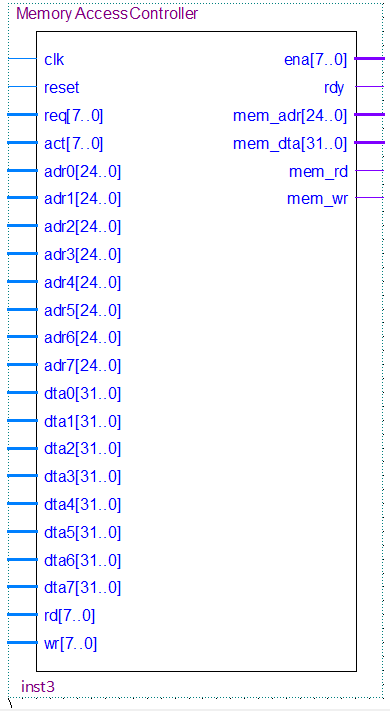
\includegraphics[width=0.3\textwidth]{Memory_Access_Controller}}
  \qquad
  \subfloat[ ][ ]{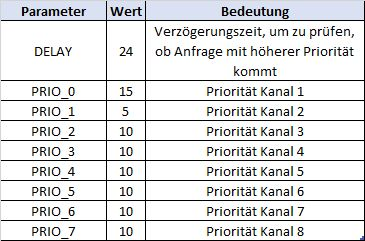
\includegraphics[width=0.4\textwidth]{Parameter_MemoryAccessController}}
  \caption[Funktionsblock MemoryAccessController mit Parameterbeschreibung]{\label{pic:Memory_Access_Controller}Funktionsblock MemoryAccessController (a) mit Parameterbeschreibung (b)}
\end{figure}



\subsection{SDRAM\_Write\_Buffer\_gen}
\label{sec:SDRAM_Write_Buffer_gen}
Mit Hilfe des in \autoref{pic:SDRAM_Write_Buffer_gen} a gezeigten Funktionsblocks SDRAM\_Write\_Buffer\_gen und den in \autoref{pic:SDRAM_Write_Buffer_gen} b aufgelisteten Parametern werden die Pixeldaten, die er vom Funktionsblock camera\_data\_mux\_gen erhält, im SDRAM gespeichert. Über mehrere FirstInFirstOut-Buffer (FIFO), die über eine Zustandsmaschine gefüllt und über eine weitere wieder geleert werden, werden die Kameradaten zwischengespeichert und sobald das Freigabesignal des MemoryAccessControllers erfolgt, werden die Daten im SDRAM gespeichert. Am Eingang cam\_data erhält der Funktionsblock die Pixeldaten und am Eingang cam\_data\_valid wird deren Gültigkeit signalisiert. Am Eingangssignal cam\_line wird die Bildzeile angegeben, aus der die aktuellen Pixel stammen.\\

\begin{figure}[h!tb]
  \centering
  \subfloat[ ][ ]{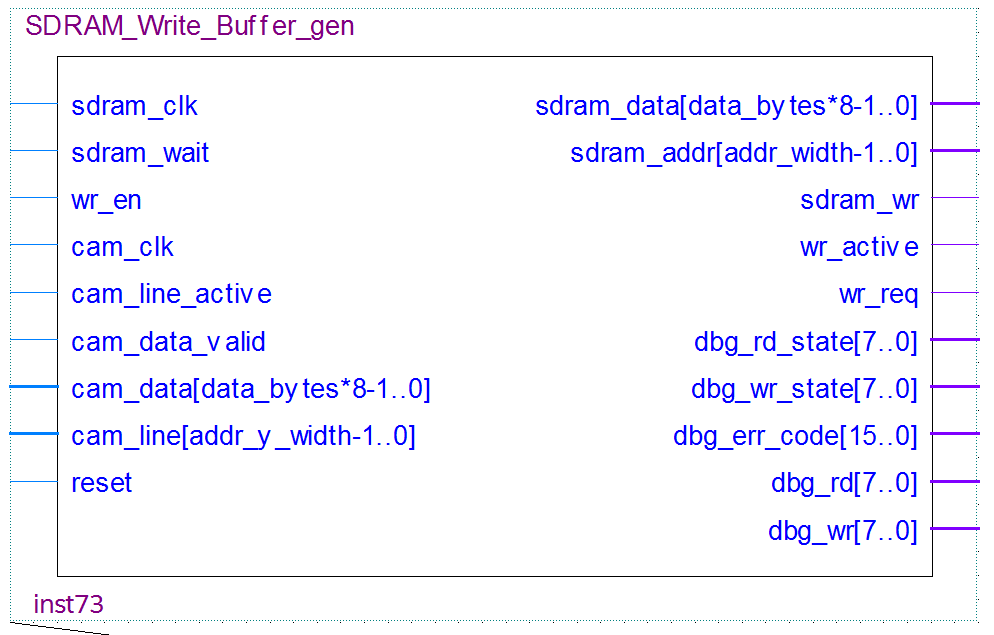
\includegraphics[width=0.5\textwidth]{SDRAM_Write_Buffer_gen}}
  \qquad
  \subfloat[ ][ ]{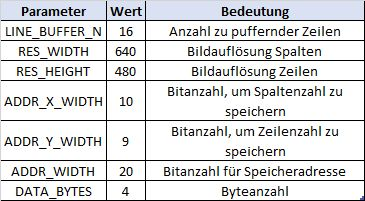
\includegraphics[width=0.4\textwidth]{Parameter_SDRAM_Write_Buffer_gen}}
  \caption[Funktionsblock SDRAM\_Write\_Buffer\_gen mit Parameterbeschreibung]{\label{pic:SDRAM_Write_Buffer_gen}Funktionsblock  SDRAM\_Write\_Buffer\_gen (a) mit Parameterbeschreibung (b)}
\end{figure}

Über die Zustandsmaschine rd\_state werden mit dem an cam\_clk anliegenden TaktsignalCLRRXCLK\_BASE die Pixeldaten in den FIFO-Buffer geschrieben. Über den Parameter LINE\_Buffer\_N kann eingestellt werden, wie viele Zeilen gepuffert werden sollen. Dazu wird pro Zeile ein FIFO-Buffer angelegt. Sind alle FIFO-Buffer gefüllt, wird die nächste Zeile erst in einen FIFO-Buffer geschrieben, wenn dieser durch das Lesen der Daten aus diesem wieder leer ist.\\ 
Das Lesen der Daten aus den FIFO-Buffern, um sie im SDRAM zu speichern, wird mit dem Takt clk\_pll am Eingang sdram\_clk und der Zustandsmaschine wr\_state ermöglicht. Es wird eine Schreibanfrage an den MemoryAccessController mittels des Signals wr\_req gesendet und sobald das Eingangssignal an wr\_en von '0' auf '1' wechselt, beginnt das Auslesen der FIFO-Buffer. Die Pixeldaten für die über den Parameter DATA\_BYTES eingestellte Anzahl an Bytes, was der Anzahl der Pixel entspricht, werden auf den Ausgang sdram\_data gelegt und auf den Ausgang sdram\_addr die dazugehörige Speicheradresse. Diese wird mittels der Komponente c\_xy\_to\_address aus der Zeile und der Spalte, die den x- und y-Koordinaten des Pixels im Bild entsprechen, berechnet und über die Parameter RES\_WIDTH und RES\_HEIGHT, die die Größe des Bildes enthalten, wird überprüft, ob das Zeilenende bzw. das Bildende erreicht wurde. Während des Schreibens der Daten auf den SDRAM wird das Signal wr\_active auf '1' gesetzt, um dem MemoryAccessController zu signalisieren, dass dieser Funktionsbaustein noch auf den SDRAM zugreift. Sollte der SDRAM beschäftigt sein und kann deshalb momentan keine Daten verarbeiten, signalisiert er dies dem Funktionsblock durch eine '1' am Eingang sdram\_wait. Dann wird gewartet, bis der SDRAM nicht mehr beschäftigt ist und das Schreiben der Pixeldaten in diesen wird fortgesetzt.



\subsection{dram}
\label{sec:dram}
Dieser Funktionsblock übernimmt die Aufgabe, Daten in den SDRAM des DE2-115-Boards zu speichern oder von diesem zu lesen. Die Schnittstellen sind in \autoref{pic:dram} abgebildet. Der Baustein arbeitet mit dem an clock anliegenden Taktsignal. Wenn am Eingang wren eine '1' anliegt werden die an data[31..0] anliegenden Daten in der Speicheradresse, die am Eingang address[16..0] anliegt, abgespeichert. Soll von SDRAM gelesen werden, wird dies über das Signal rden signalisiert. Ist dieses auf '1' gesetzt, werden die Daten aus der an address[16..0] anliegenden Speicheradresse gelesen und auf den Ausgang q[31..0] gelegt. Das Schreiben und Lesen des SDRAM erfolgt über die Komponente altsyncram aus der altera\_mf Bibliothek.

\begin{figure}[htbp]
	\begin{center}
	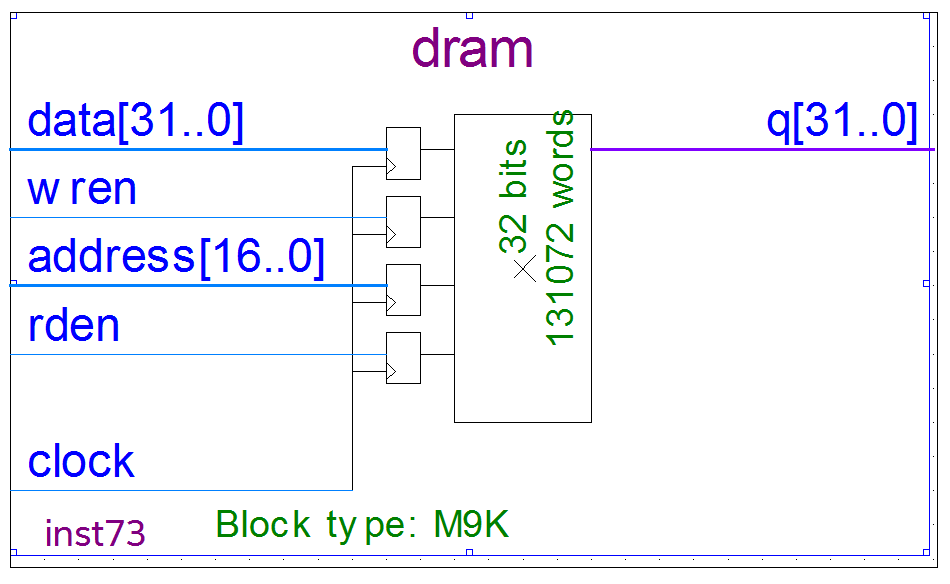
\includegraphics[width = 0.3\textwidth]{dram}
	\caption [Funktionsblock dram]{\label{pic:dram}Funktionsblock dram}
	\end{center}
\end{figure}



\subsection{sdram\_controller\_latency1}
\label{sec:sdram_controller_latency1}
Der in \autoref{pic:sdram_controller_latency 1} dargestellte Funktionsblock sdram\_latency\_controller1 hat prinzipiell die gleiche Aufgabe wie der dram Funktionsblock. Auch er speichert die Pixeldaten in den SDRAM. An den Eingängen az\_read und az\_write wird signalisiert, ob gelesen oder geschrieben werden soll. Wenn geschrieben werden soll, werden die Daten des Eingang az\_writedata an der Adresse, die an az\_address anliegt, gespeichert. Soll gelesen werden, werden die an der angelegten Speicheradresse liegenden Daten auf den Ausgang za\_readdata gelegt und durch das Signal za\_readdatavalid wird deren Gültigkeit angezeigt. Der Baustein arbeitet mit dem an der Eingangsschnittstelle az\_clk  anlegten Taktsignal clk\_pll. Mittels des Ausgangssignals za\_waitrequest signalisiert der sdram\_controller\_latency1, dass der auf den Speicher zugreifende Funktionsblock warten muss, da er gerade beschäftigt ist und die Anfrage derzeit nicht bearbeiten kann. Über die restlichen Ausgänge erfolgt das Schreiben der Daten in den Speicher bzw. über das INOUT-Signal za\_dq erfolgt auch das Auslesen der Daten aus diesem.

\begin{figure}[htbp]
	\begin{center}
	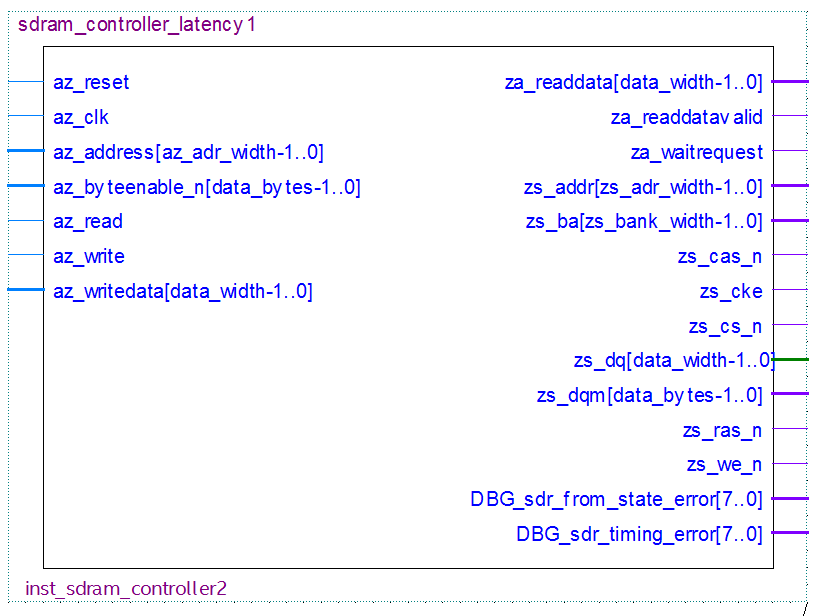
\includegraphics[width = 0.5\textwidth]{sdram_controller_latency_1}
	\caption [Funktionsblock sdram\_controller\_latency 1]{\label{pic:sdram_controller_latency 1}Funktionsblock sdram\_controller\_latency 1}
	\end{center}
\end{figure}



\subsection{SDRAM\_Read\_Buffer\_gen}
\label{sec:SDRAM_Read_Buffer_gen}
Die Aufgabe des in \autoref{pic:SDRAM_Read_Buffer_gen} a dargestellten SDRAM\_Read\_Buffer\_gen ist es, die Daten eines Bildes vom SDRAM zu lesen und diese einem nachfolgenden Funktionsbaustein zur Verfügung zu stellen. Er wird genutzt, um die Pixeldaten über den VGA-Ausgang an einem Monitor auszugeben, sodass das gespeicherte Bild wiedergegeben werden kann. Die Bedeutungen der Parameter des Funktionsblocks sind in \autoref{pic:SDRAM_Read_Buffer_gen} b beschrieben.\\

\begin{figure}[h!tb]
  \centering
  \subfloat[ ][ ]{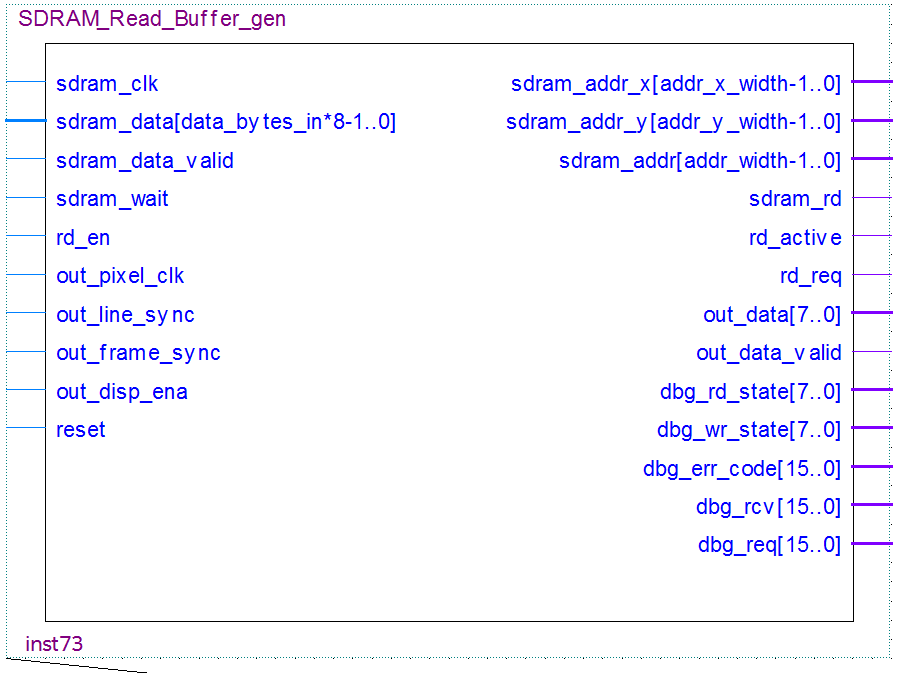
\includegraphics[width=0.5\textwidth]{SDRAM_Read_Buffer_gen}}
  \qquad
  \subfloat[ ][ ]{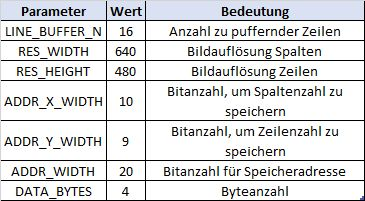
\includegraphics[width=0.4\textwidth]{Parameter_SDRAM_Write_Buffer_gen}}
  \caption[Funktionsblock SDRAM\_Read\_Buffer\_gen mit Parameterbeschreibung]{\label{pic:SDRAM_Read_Buffer_gen}Funktionsblock  SDRAM\_Read\_Buffer\_gen (a) mit Parameterbeschreibung (b)}
\end{figure}

Das Lesen der Daten vom SDRAM erfolgt über die Zustandsmaschine rd\_state, die mit dem Takt clk\_pll an der Eingangsschnittstelle sdram\_clk arbeitet. Über den Ausgang rd\_req wird eine Zugriffsanfrage an den MemoryAccessController geschickt und durch den Ausgang sdram\_rd wird signalisiert, dass vom SDRAM Daten gelesen werden möchten. Der MemoryAccessContoller signalisiert am Eingang rd\_en, dass nun auf den SDRAM zugegriffen werden darf. Dann erfolgt das Lesen der Daten, deren Gültigkeit durch das Signal am Eingang sdram\_data\_valid bestätigt wird. Dabei werden die einzelnen Zeilen in einer über den Parameter LINE\_BUFFER\_N einstellbaren Anzahl an FIFO-Buffern gepuffert, wobei pro FIFO-Buffer eine Zeile gespeichert wird. Wenn alle beschrieben wurden, wird das Auslesen des SDRAM solange unterbrochen, bis ein FIFO-Buffer ausgelesen ist.\\
Über die Zustandsmaschine wr\_state erfolgt die Ausgabe der in FIFO-Buffern gespeicherten Pixeldaten mit dem Takt vga\_pixel\_clk  am Eingang out\_pixel\_clk. Dabei werden pro Takt die Daten für ein Pixel auf den Ausgang out\_data gelegt und durch eine '1' auf dem Ausgangssignal out\_data\_valid werden diese als gültig gekennzeichnet. Damit die Pixeldaten über VGA auch an der richtigen Stelle und zum richtigen Zeitpunkt ausgegeben werden, wird die Datenausgabe zusätzlich über die Signale an den Eingängen out\_line\_sync, out\_line\_frame\_sync und out\_disp\_ena  gesteuert, die mit teils invertierten Signalen des vga\_controllers (Kapitel \ref{sec:vga_controller} \nameref{sec:vga_controller}) gespeist werden. Durch einen Signalwechsel vom Signal out\_frame\_sync von '0' auf '1' wird angekündigt, dass die Ausgabe eines neuen Bildes in ein paar Takten beginnen kann. Während das Signal out\_disp\_ena auf '1' ist, erfolgt die Ausgabe der Pixel. Das Signal  out\_line\_sync wird zwar aufgenommen, allerdings nicht benutzt.



\subsection{vga\_controller}
\label{sec:vga_controller}
Der Funktionsblock vga\_controller von Scott Larson hat die Aufgabe, die Ausgabe der Pixeldaten über den VGA-Ausgang zu steuern \cite{Digi-Key}. Dieser in \autoref{pic:vga_controller} a dargestellt Block arbeitet mit dem an dem Eingang pixel\_clk angelegten Takt vga\_pixel\_clk, der 25 Mhz beträgt. Zur Steuerung und Synchronisierung der Pixelausgabe werden die low-aktiven Signale h\_sync, v\_sync und das Signal disp\_ena erzeugt, deren Verhalten über die in \autoref{pic:vga_controller} b beschriebenen Parameter eingestellt wird.\newline

\begin{figure}[h!tb]
  \centering
  \subfloat[ ][ ]{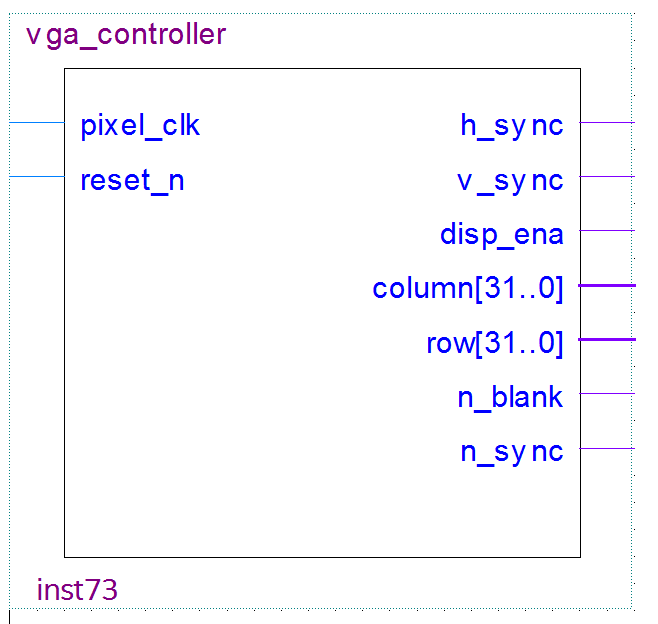
\includegraphics[width=0.3\textwidth]{vga_controller}}
  \qquad
  \subfloat[ ][ ]{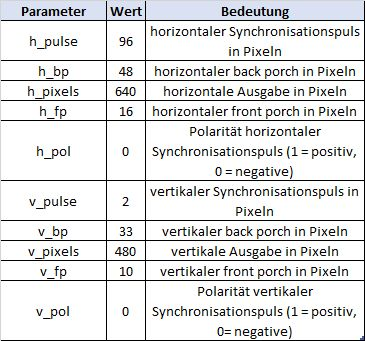
\includegraphics[width=0.4\textwidth]{Parameter_vga_controller}}
  \caption[Funktionsblock vga\_controller mit Parameterbeschreibung]{\label{pic:vga_controller}Funktionsblock vga\_controller (a) mit Parameterbeschreibung (b)}
\end{figure}

Zu Beginn der ersten Zeile wechselt das Signal disp\_ena von '0' auf '1'. Dann werden die Pixeldaten für die erste Zeile übertragen. Wurden die Daten für die erste Zeile ausgegeben, geht das Signal disp\_ena wieder von '1' auf '0'  zurück. Nach ein paar Takten signalisiert das h\_sync durch einen kurzen '0' Impuls, dass die Übertragung der nächsten Zeile in wenigen Takten beginnen kann. Für die Zeit der Übertragung der Zeile ist das Signal disp\_ena wieder auf '1' gesetzt. Dies wird solange wiederholt, bis ein komplettes Bild ausgegeben wurde und das Signal v\_sync durch einen '0' Impuls ankündigt, dass ein neues Bild ausgegeben werden kann.
\clearpage
%Stand zu Bearbeitungsbeginn Ende





%Anfang Eindimensionale Positionserkennung
\section{Eindimensionale Positionserkennung verschiedener Objekte}
\label{sec:Eindimensionale Positionserkennung}
Aufbauend auf den schon vorhandenen Funktionen und den in Kapitel \ref {sec:Stand zu Bearbeitungsbeginn} beschriebenen Funktionsblöcken, war es das Ziel, die eindimensionale Positionserkennung von Punkten und Linien und die Ausgabe einer Zeile über den VGA-Ausgang auf einen Monitor zu erreichen. Um dies umzusetzen, wurde zuerst ein Funktionsblock geschrieben, der eine einzige Bildzeile ausgibt, in der nach einem Objekt gesucht werden kann. Anschließend wurden verschiedene Funktionsblöcke entworfen, die die Suche nach einem Objekt in dieser einen Zeile durchführen.



\subsection{Extraktion einer Bildzeile}
\label{sec:Extrahieren einer Bildzeile}
Um das Ziel der eindimensionalen Positionserkennung von Objekten, also Punkten und Linien, zu erreichen, wurde als erstes die Pufferung und anschließende Ausgabe von genau einer Zeile benötigt. Dazu ist der Funktionsblock SINGLE\_LINE\_READ\_BUFFER entworfen worden, der mit zusätzlicher äußerer Beschaltung eine vorgegebene Bildzeile puffert und ausgibt, damit diese über den VGA-Ausgang auf dem angeschlossenen Monitor dargestellt werden kann. Um diesen Funktionsblock zu realisieren, ist der in Kapitel \ref{sec:SDRAM_Read_Buffer_gen} beschriebene Funktionsblock SDRAM\_Read\_Buffer\_gen als Vorlage genutzt worden.\\

\begin{figure}[h!tb]
  \centering
  \subfloat[ ][ ]{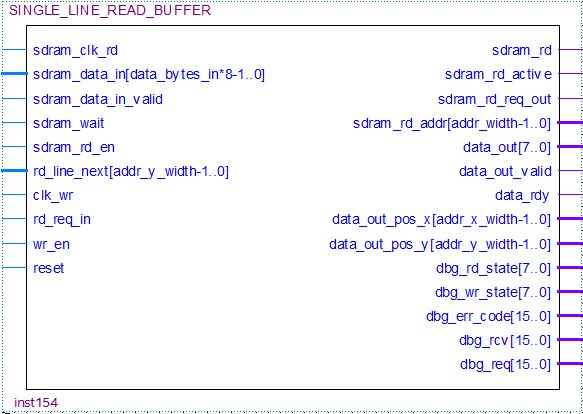
\includegraphics[width=0.4\textwidth]{SINGLE_LINE_READ_BUFFER-191211_bearbeitet}}
  \qquad
  \subfloat[ ][ ]{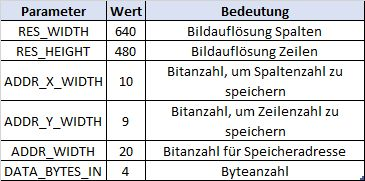
\includegraphics[width=0.4\textwidth]{Parameter_SINGLE_LINE_READ_BUFFER}}
  \caption[Funktionsblock SINGLE\_LINE\_READ\_BUFFER mit Parameterbeschreibung]{\label{pic:SINGLE_LINE_READ_BUFFER}Funktionsblock SINGLE\_LINE\_READ\_BUFFER (a) mit Parameterbeschreibung (b)}
\end{figure}

Auf Grundlage dieses Funktionsblocks wurden einige Funktions- und Signalnamensänderungen vorgenommen, wobei die grundlegende Funktion die gleiche geblieben ist. So wird nun nur noch ein FIFO-Buffer erzeugt, in dem eine Zeile gespeichert wird, die durch das Signal an der Eingangsschnittstelle rd\_line\_next vorgegeben wird. Zudem werden die x- und y-Koordinaten der Pixel, die aus dem Funktionsblock ausgegeben werden, auf die Ausgangssignale data\_out\_pos\_x und data\_out \_pos\_y gelegt. Das Lesen der Daten vom SDRAM, dessen Schreiben in den FIFO-Buffer und das Auslesen dieser Daten aus diesem erfolgt weiterhin über die beiden Zustandsmaschinen rd\_state mit dem Takt clk\_pll am Eingang sdram\_clk\_rd (\autoref{pic:Zustandsmaschinen des SINGLE_LINE_READ_BUFFER's} a) und wr\_state mit dem Takt vga\_pixel\_clk am Eingang clk\_wr (\autoref{pic:Zustandsmaschinen des SINGLE_LINE_READ_BUFFER's} b), wobei hier einige Namensanpassungen von Signalen vorgenommen wurden. Über die Zustandsmaschine rd\_state werden die Pixeldaten einer Zeile eingelesen und in den FIFO-Buffer geschrieben, sobald über das Eingangssignal rd\_req\_in eine Anfrage zum Lesen einer Zeile erfolgt. Nach dem Einlesen der Daten ist es möglich, die Daten wieder aus dem FIFO-Buffer auszulesen und pro Takt die Daten eines Pixels auf den Ausgang data\_out[7..0] zu legen. Dies geschieht, sobald am Eingangssignal wr\_en eine '1' anliegt. Dabei werden, wie oben erwähnt, zusätzlich die x- und y-Koordinaten der Pixel ausgegeben. Die Bedeutung der Parameter ist in \autoref{pic:SINGLE_LINE_READ_BUFFER} b beschrieben, wobei der Wert von DATA\_BYTES\_IN auf den Wert einzustellen ist, der der Ausgabe der Bytes pro Takt aus dem SDRAM entspricht.\newline

\begin{figure}[h!tb]
  \centering
  \subfloat[ ][ ]{\includegraphics[width=0.275\textwidth]{SINGLE_LINE_READ_BUFFER-rd_state}}
  \qquad
  \subfloat[ ][ ]{\includegraphics[width=0.275\textwidth]{SINGLE_LINE_READ_BUFFER-wr_state}}
  \caption[Zustandsmaschinen des SINGLE\_LINE\_READ\_BUFFER's]{\label{pic:Zustandsmaschinen des SINGLE_LINE_READ_BUFFER's}Zustandsmaschinen rd\_state zum Lesen der Daten aus dem SDRAM (a) und dem Puffern dieser in einem FIFO-Buffer; Zustandsmaschine er\_state zum Auslesen des FIFO-Buffers und das Schreiben der Daten auf den Ausgang (b)}
\end{figure}

Um die Darstellung dieser einzelnen Bildzeile auf Monitor auch in der entsprechenden Monitorzeile zu ermöglichen, war noch eine äußere Beschaltung notwendig, damit der SINGLE\_LINE\_READ\_BUFFER die richtige Zeile puffert und diese Zeile zum richtigen Zeitpunkt wieder ausgibt. Zur Bestimmung, welche Bildzeile eingelesen werden soll, wurde der Funktionsblock CTU\_RTU\_LINE geschrieben. Dieser Funktionsblock gibt als Ausgabewert die auszugebende Zeile aus, die defaultmäßig auf die erste Bildzeile(entspricht y-Koordinate 0) gestellt ist. Durch das Betätigen des Tasters KEY[2] wird dieser Wert jeweils um eins erhöht und über RESET kann er wieder zurückgesetzt werden. Zur Bestimmung des Zeitpunkts zum Einlesen der Daten in den FIFO-Buffer des SINGLE\_LINE\_READ\_Buffers und deren Ausgabe wurden die Signale h\_sync, v\_sync und disp\_ena des vga\_controllers genutzt. Mittels des Flankenwechsels von '0' auf '1' des invertierten v\_sync Signals wird das Einlesen der Bildzeile gestartet. Zur Ausgabe der Bildzeile werden die Signale h\_sync und disp\_ena genutzt. Allerdings gab es anfänglich Schwierigkeiten, das Eingangssignal wr\_en des SINGLE\_LINE\_READ\_Buffers zum richtigen Zeitpunkt auf '1' zu setzen, damit die Ausgabe der Bildzeile erfolgt. Zuerst wurde versucht, über einen selbsgeschriebenen Zählerbaustein CTU\_VGA die Zeile zu bestimmen, die gerade am VGA-Ausgang ausgegeben wurde. Der Zeilenwert wurde um 1 erhöht, sobald das invertierte Signal h\_sync des vga\_controllers einen Flankenwechsel von '0' auf '1' aufwies und zurückgesetzt, durch den Flankenwechsel des invertierten v\_sync-Signals von '0' auf '1'. Mit Hilfe eines geschriebenen Vergleichers wurde das wr\_en-Signal auf '1' gesetzt, sobald die gezählte Zeilennummer des CTU\_VGA der Zeilennummer des CTU\_RD\_LINE entsprach. Diese Beschaltung führte dazu, dass ein x- sowie y-Versatz in der Bildausgabe dieser Zeile vorhanden war. So wurden ca. die ersten 100 Pixel der Zeile nicht ausgegeben und die Ausgabe von der Bildzeile mit der y-Koordinate 0 erfolgte in der letzten Monitorzeile.\\

Als Grund des x-Versatzes stellte sich heraus, dass das wr\_en Signal schon auf '1' gesetzte wurde und somit der Funktionsblock SINGLE\_LINE\_READ\_BUFFER die Pixeldaten der Bildzeile  ausgab, bevor die Ausgabe über den VGA-Ausgang begann. Die Ausgabe einer Bildzeile über VGA erfolgt nur in der Zeit, in der das Signal disp\_vga auf '1' gesetzt ist. Deshalb wurde zwischen dem Ausgang des Vergleichers und der Eingangsschnittstelle wr\_en des SINGLE\_LINE\_READ\_Buffers ein UND-Glied geschaltet, das mit dem Ausgangssignal des Vergleichers und dem Singal disp\_ena des vga\_controllers beschaltet wurde. Jetzt erfolgte die Ausgabe erst, wenn beide Signale auf '1' standen, wodurch es zu keinem x-Versatz mehr bei der Ausgabe der Pixel kam.\newline

\begin{figure}[htbp]
	\begin{center}
	\includegraphics[width = 0.7\textwidth]{vga_timing}
	\caption [Verhalten der Signale des vga\_controllers]{\label{pic:vga_timing}Verhalten der Signale des vga\_controllers \cite{Digi-Key}}
	\end{center}
\end{figure}

Um das Problem mit dem y-Versatz zu lösen, wurde auf Vorschlag von Herrn Prof. Dr. Gick das Verhalten der Signale des vga\_controllers nochmals genauer geprüft, welches in \autoref{pic:vga_timing} dargestellt ist. Zusätzlich wurde das Verhalten der Signale h\_sync und v\_sync mit einem Oszilloskop der Firma Tektronix, dem TDS 3014C 100MHz, aufgezeichnet. Dieses aufgezeichnete Verhalten bestätigte das in \autoref{pic:vga_timing} gezeigte Verhalten dieser Signale. Die Signale h\_sync und v\_sync sind low aktiv, wie es auch der Parameterbeschreibung in \ref{sec:vga_controller} \nameref{sec:vga_controller} in \autoref{pic:vga_controller} b des vga\_controllers zu entnehmen ist. Die Parameter h\_pol und v\_pol sind auf '0' gestellt, wodurch die Signale h\_sync und v\_sync mit negativer Logik arbeiten. Das Signal h\_sync ist für die Zeit der Ausgabe der Pixel einer Zeile und den Abschnitt Front Porch auf high. Anschließend ist es für den Abschnitt Sync Pulse auf low, danach wird es im Abschnitt Back Porch wieder auf high gesetzt. Das Signal v\_sync ist für den Abschnitt Display und Front Porch auf high gesetzt. Danach wird es für den Abschnitt Sync Pulse auf low und abschließend im Abschnitt Back Porch wieder auf high gesetzt. In der \autoref{pic:vga_timing_2} wird gezeigt, wie viele Takte bzw. Zeilen die jeweiligen Abschnitte bei einer Bildauflösung von 640x480 Pixeln und einer Taktfrequenz von 25,175 MHz auf high oder low gesetzt sind. Zudem lässt sich aus der \autoref{pic:vga_timing} herauslesen, dass das Signal disp\_ena im Abschnitt  Display auf high gesetzt und ansonsten low ist.\newline

\begin{figure}[htbp]
	\begin{center}
	\includegraphics[width = 1\textwidth]{vga_timing_2}
	\caption [Anzahl der Takte der Abschnitte der Signale des vga\_controllers]{\label{pic:vga_timing_2}Anzahl der Takte der Abschnitte der Signale des vga\_controllers (\cite{Digi-Key}) }
	\end{center}
\end{figure}

Anhand der gewonnenen Erkenntnisse des Verhaltens der Signale des vga\_controllers wurden Anpassungen an der Erzeugung der Signale wr\_en und rd\_line\_next für den SINGLE\_LINE\_READ\_BUFFER vorgenommen. So wurde ein neuer Zähler CTU\_VGA\_V2 entworfen, um die Zeile, in der sich die VGA-Ausgabe befindet, zu zählen. Dieser berücksichtigt zusätzlich als Parameter die Zeiten Front Porch, Sync Pulse und Back Porch des v\_sync Signals. Dadurch war es nun möglich, eine im SINGLE\_LINE\_READ\_BUFFER gepufferte Bildzeile zum richtigen Zeitpunkt auszugeben, sodass sie auch in der entsprechenden Monitorzeile ausgegeben wurde, wie es in \autoref{pic:Ausgabe einer Zeile über VGA} zu sehen ist.

\begin{figure}[htbp]
	\begin{center}
	\includegraphics[width = 0.4\textwidth]{IMG_20191217_103944_bearbeitet_2}
	\caption[Ausgabe einer Zeile über VGA]{\label{pic:Ausgabe einer Zeile über VGA}Ausgabe einer Zeile über VGA}
	\end{center}
\end{figure}

Des Weiteren wurde, nach Hinweis von Prof. Dr. Gick asynchrone Signale einzusynchronisieren und das Zählen der Zeile der VGA-Ausgabe über eine Zustandsmaschine zu realisieren, das asynchrone Eingangssignal des Tasters KEY[2] mit Hilfe des Bausteins SYNCHRONIZATION einsynchronisiert und der Funktionsblock CTU\_VGA\_V2 in den Funktionsblock CTU\_VGA\_V3\_state\_machine umgewandelt, bei dem das Zählen der Zeile der VGA-Ausgabe nun über eine Zustandsmaschine erfolgt. In \autoref{pic:SINGLE_LINE_READ_BUFFER-Beschaltung} sind die genutzten Funktionsblöcke und die logischen Verbindungen für die beiden Signale wr\_en und rd\_line\_next dargestellt. Diese sind über die Verbindungen mit den Label SLRD\_wr\_en und SLRD\_rd\_line\_next mit den entsprechenden Eingangsschnittstellen des SINGLE\_LINE\_READ\_BUFFERs verbunden.\newline

\begin{figure}[htbp]
	\begin{center}
	\includegraphics[width = \textwidth]{SLRB_wr_en_20200107_bearbeitet}
	\caption[Erzeugung der Eingangssignale rd\_line\_next und wr\_en des SINGLE\_LINE\_READ\_BUFFERS ]{\label{pic:SINGLE_LINE_READ_BUFFER-Beschaltung}Erzeugung der Eingangssignale rd\_line\_next und wr\_en des SINGLE\_LINE\_READ\_BUFFERS }
	\end{center}
\end{figure}

Zusätzlich wurde der in \autoref{pic:GLG} a gezeigte Funktionsblock GREY\_LEVEL\_GENERATOR entworfen, um die Farbintensität der Zeilen, die nicht vom SINGLE\_LINE\_READ\_BUFFER über VGA ausgegeben werden, stufenweise zu verändern (\autoref{pic:GLG}). Dies wurde genutzt, um die extrahierte Zeile auf dem Monitor besser zu erkennen, da das aufgenommene Kamerabild anfangs einen dunklen Hintergrund besaß, da noch nicht mit einen weißen Blatt Papier als Standardhintergrund gearbeitet wurde.

\begin{figure}[h!tb]
  \centering
  \subfloat[ ][ ]{\includegraphics[width=0.4\textwidth]{GREY_LEVEL_GENERATOR-191211}}
  \qquad
  \subfloat[ ][ ]{\includegraphics[width=0.4\textwidth]{IMG_20200108_105613_bearbeitet}}
  \caption[Funktionsblock GREY\_LEVEL\_Generator]{\label{pic:GLG}Funktionsblock GREY\_LEVEL\_Generator (a) und mit dem GREY\_LEVEL\_GENERATOR bearbeitete Ausgabe}
\end{figure}



\subsection{Eindimensionale Positionserkennung eines isolierten Punktes}
\label{sec:Eindimensionale Positionserkennung eines isolierten Punkts}
Basierend auf der Extraktion einer Bildzeile und deren Ausgabe mittels des SINGLE\_LINE\_READ\_BUFFERs über VGA erfolgte die Implementierung einer eindimensionalen Objekterkennung für einen isolierten Punkt. Dabei beruht das Konzept der Positionserkennung auf dem Mitlesen der Pixelwerte der isolierten Zeile und der Suche nach einem isolierten Punkt mittels mathematischer Bildoperationen.\newline

\begin{figure}[h!tb]
  \centering
  \subfloat[ ][ ]{\includegraphics[width=0.4\textwidth]{ISOLATED_POINT_DETECTION-191211_bearbeitet}}
  \qquad
  \subfloat[ ][ ]{\includegraphics[width=0.4\textwidth]{Parameter_IPD}}
  \caption[Funktionsblock ISOLATED\_PONIT\_DETECTION mit Parameterbeschreibung]{\label{pic:ISOLATED_POINT_DETECTION}Funktionsblock ISOLATED\_PONIT\_DETECTION (a) mit Parameterbeschreibung (b)}
\end{figure}

Die Umsetzung der Positionserkennung erfolgte durch den Entwurf des Funktionsblocks ISOLATED\_POINT\_DETECTION, der in \autoref{pic:ISOLATED_POINT_DETECTION} a dargestellt ist. Die Berechnung und Suche nach einem isolierten Punkt erfolgt mit Hilfe der in Kapitel \ref{sec:Mathematische Operationen zur Bilddatenverarbeitung} beschriebenen Faltung mit der aus der 2. Ableitung der eindimensionalen Bildfunktion f(x) resultierenden Gewichtungsmatrix. Anhand der Ergebnisse der Faltungssumme an jeder Stelle einer Zeile kann darauf geschlossen werden, ob ein isolierter Punkt vorliegt oder nicht. Dafür müssen die Werte Pixel eingelesen und die Faltung durchgeführt werden, was über die in \autoref{pic:Zustandsmaschine ISOLATED_POINT_DETECTION} gezeigte Zustandsmaschine erfolgt.\newline

\begin{figure}[htbp]
	\begin{center}
	\includegraphics[width = 0.25\textwidth]{ISOLATED_PONIT_DETECTION}
	\caption[Zustandsmaschine ISOLATED\_PONIT\_DETECTION]{\label{pic:Zustandsmaschine ISOLATED_POINT_DETECTION}Zustandsmaschine ISOLATED\_POINT\_DETECTION}
	\end{center}
\end{figure}

Im ersten Zustand wait\_for\_first\_pixel\_state wird der Pixelwert, der am Eingang data\_[7..0] anliegt, eingelesen, sobald das Signal am Eingang data\_in\_valid von '0' auf '1' wechselt. Dieser Wert entspricht dem Pixel an Stelle f(x-1). Zudem wird die x-Koordinate des Pixles am Eingang x\_pos\_in[9..0] aufgenommen, damit bei einem gefundenen isolierten Punkt die Position ausgegeben werden kann. Zudem erfolgt der Wechsel in den zweiten Zustand wait\_for\_second\_pixel\_data\_state. In diesem wird der Wert und die x-Koordinate des zweiten Pixels eingelesen, der dem Wert an Stelle f(x) entspricht und in den dritten Zustand wait\_for\_third\_pixel\_state gewechselt, in dem der Wert für das dritte Pixel (f(x+1)) sowie dessen x-Koordinate aufgenommen werden. Anschließend erfolgt der Wechsel in den Zustand conv\_state.\\
Im conv\_state Zustand wird das Ergebnis der Faltungsumme für die ersten drei eingelesenen Pixeldaten mit der Gewichtungsmatrix der 2. Ableitung berechnet. Die Berechnung ist in \autoref{pic:Programmausschnitt zur Berechnung der Faltung} dargestellt. Da das Faltungsergebnis auch ein negatives Ergebnis sein kann, muss der Datentyp std\_logic\_vector der Pixeldaten in einen signed-Datentyp umgewandelt werden und zusätzlich muss die Länge der Daten angepasst werden. Dies geschieht über die selbstgeschriebene Funktion std\_to\_sig\_resize, in der zunächst der Datentyp std\_logic\_vector in den unsigned-Datentyp umgewandelt, anschließend auf eine vorgegebene Größe verlängert und dann in den signed-Datentyp gewandelt wird. Falls das Ergebnis der Faltung einen Schwellwert, der über den in \autoref{pic:ISOLATED_POINT_DETECTION} b beschriebenen Parameter THRESHOLD eingestellt wird, überschreitet, ist ein isolierter Punkt gefunden. Dann wird dies am Ausgang det\_obj\_out durch einen Signalwechsel von '0' auf '1' signalisiert. Zudem wird die x-Koordinate des gefundenen Punktes über den Ausgang det\_obj\_x\_pos\_out ausgegeben. Wird der Schwellwert nicht überschritten, werden die Daten für das nächste Pixel eingelesen. Dadurch wird das Pixel f(x) zum Pixel f(x-1), das Pixel f(x+1) zum Pixel f(x) und das neu aufgenommene zum Pixel f(x+1). Das vorherige Pixel f(x-1) fällt heraus, da es zur Berechnung nicht mehr benötigt wird. Anschließend wird im nächsten Takt erneut die Faltungssumme berechnet. Dieser Ablauf wird conv\_state solange wiederholt, bis ein isolierter Punkt gefunden oder das Zeilenende erreicht wurde, das durch den Parameter RES\_WIDTH bestimmt wird, welcher der Breite einer Bildzeile entspricht.\newline

\begin{figure}[htbp]
	\begin{center}
	\includegraphics[width = 0.8\textwidth]{convolution_2_Ableitung}
	\caption[Programmausschnitt zur Berechnung der Faltung]{\label{pic:Programmausschnitt zur Berechnung der Faltung}Programmausschnitt zur Berechnung der Faltung}
	\end{center}
\end{figure}

\begin{figure}[h!tb]
  \centering
  \subfloat[ ][ ]{\includegraphics[width=0.4\textwidth]{IMG_20191217_104036_bearbeitet_2}}
  \qquad
  \subfloat[ ][ ]{\includegraphics[width=0.4\textwidth]{IMG_20191217_104107_gedreht_bearbeitet}}
  \caption[Darstellung eines isolierten Punktes in einer Bildzeile und Ausgabe der x-Koordinate auf dem FPGA-Board]{\label{pic:isolierter_Punkt}Darstellung eines isolierten Punktes in einer Bildzeile (a) und Ausgabe der x-Koordinate auf dem FPGA-Board (b)}
\end{figure}

Um die Funktion des ISOLATED\_POINT\_DETECTION Funktionsblocks zu testen, wurde der in \autoref{pic:ISOLATED_POINT_GENERATOR} a gezeigte Funktionsblock ISOLATED\_POINT\_GENERATOR geschrieben. Dieser erzeugt in einer Zeile an einer vorgegebenen x-Koordinate einen Punkt mit einer einstellbaren Intensität, wie es in \autoref{pic:isolierter_Punkt} a zu sehen ist. Beides ist über die in \autoref{pic:ISOLATED_POINT_GENERATOR} b beschriebenen Parameter einstellbar. Als Hintergrund für das von der Kamera aufgenommene Bild wurde ein weißes Blatt Papier genutzt. Mithilfe des ISOLATED\_POINT\_GENERATOR wurde dann in der Zeile, die der SINGLE\_LINE\_READ\_BUFFER extrahiert, eine schwarzer Punkt an der x-Koordinate 150 erzeugt. Dieser schwarze Punkt wurde als isolierter Punkt erkannt und die eingestellte Position korrekterweise als x-Koordinate auf der Siebensegmentanzeige des FPGA-Boards hexadezimal dargestellt (\autoref{pic:isolierter_Punkt} b). Ist anstatt eines schwarzen Punktes ein Punkt mit geringerer Intensität erzeugt worden, ist dieser nicht als isolierter Punkt erkannt worden, wenn das Ergebnis der Faltung nicht den eingestellten Schwellwert im ISOLATED\_POINT\_DETECTION-Funktionsblock überschritten hat.\\
Des Weiteren wurde getestet, ob der Funktionsblock eine Folge von schwarzen Pixeln auf weißem Hintergrund bzw. die Kante der Linie nicht als isolierten Punkt erkennt. Dafür wurde auf das weiße Papier eine schwarze Linie gezeichnet, die der Funktionsblock wie gewünscht nicht als isolierten Punkt erkennt. War der Schwellwert allerdings niedriger als 256 eingestellt, wurde teilweise die Kante einer Linie als isolierter Punkt erkannt.

\begin{figure}[h!tb]
  \centering
  \subfloat[ ][ ]{\includegraphics[width=0.4\textwidth]{ISOLATED_POINT_GENERATOR-191211_bearbeitet}}
  \qquad
  \subfloat[ ][ ]{\includegraphics[width=0.4\textwidth]{Parameter_IPD}}
  \caption[Funktionsblock ISOLATED\_POINT\_GENERATOR mit Parameterbeschreibung]{\label{pic:ISOLATED_POINT_GENERATOR}Funktionsblock ISOLATED\_POINT\_GENERATOR (a) mit Parameterbeschreibung (b)}
\end{figure}



\subsection{Eindimensionale Positionserkennung mehrerer isolierter Punkte}
\label{sec:Eindimensionale Positionserkennung mehrerer isolierter Punkte}
Nach der Positionserkennung eines isolierten Punktes wurde die Erkennung so erweitert, dass mehrere isolierte Punkte als Objekte in einer Zeile erkannt werden können. Dazu wurde der Funktionsblock ISOLATED\_POINT\_DETECTION\_2 (\autoref{pic:ISOLATED_POINT_DETECTION_2} a) entworfen. Das Grundkonzept dieses Funktionsblocks ist gleich geblieben. So werden weiterhin die Daten der Zeile, die der SINGLE\_LINE\_READ\_BUFFER für die Ausgabe über VGA ausgibt, mitgelesen und über eine Zustandsmaschine aufgenommen und ausgewertet. \\

\begin{figure}[h!tb]
  \centering
  \subfloat[ ][ ]{\includegraphics[width=0.4\textwidth]{ISOLATED_POINT_DETECTION_2-191211_bearbeitet}}
  \qquad
  \subfloat[ ][ ]{\includegraphics[width=0.4\textwidth]{Parameter_IPD_2}}
  \caption[Funktionsblock ISOLATED\_PONIT\_DETECTION\_2 mit Parameterbeschreibung]{\label{pic:ISOLATED_POINT_DETECTION_2}Funktionsblock ISOLATED\_PONIT\_DETECTION\_2 (a) mit Parameterbeschreibung (b)}
\end{figure}

Dieser Funktionsblock arbeitet grundsätzlich mit der gleichen Zustandsmaschine wie der ISOLATED\_POINT\_DETECTION-Funktionsblock, die in \autoref{pic:Zustandsmaschine ISOLATED_POINT_DETECTION_2} zu sehen ist. In den Zuständen wait\_for\_first\_pixel\_state, wait\_for\_second\_pixel\_state und wait\_for\_third\_pixel\_state werden die Daten der ersten drei Pixel einer Zeile sowie deren x-Koordinate eingelesen.\\
Im Zustand conv\_state wird die Faltungssumme für das Pixel an der Stelle f(x) aus den Intensitätswerten der Pixel und der in Kapitel \ref{sec:Mathematische Operationen zur Bilddatenverarbeitung} beschriebenen Gewichtungsmatrix der 2. Ableitung auf die gleiche Weise wie beim Funktionsblock ISOLATED\_POINT\_DETECTION in Kapitel \ref{sec:Eindimensionale Positionserkennung eines isolierten Punkts} berechnet. Dabei entspricht das im Zustand  wait\_for\_first\_pixel\_state eingelesene Pixel dem Pixel an der Stelle f(x-1), das aus Zustand wait\_for\_second\_pixel\_state dem Pixel an Stelle f(x) und das im Zustand wait\_for\_third\_pixel\_state eingelesene dem Pixel an Stelle f(x+1). Überschreitet des Ergebnis der Faltung an dieser Stelle den über den Parameter THRESHOLD eingestellten Schwellwert, ist ein isolierter Punkt gefunden worden. Ist dies der Fall, wird der Zähler det\_obj\_cnt\_out um eins erhöht und zudem signalisiert der Ausgang det\_obj\_out[0] durch einen Signalwechsel von '0' auf '1', dass ein Objekt gefunden wurde. Wurde kein isolierter Punkt gefunden oder sind noch nicht die über den Parameter NUMBERS\_OF\_OBJECTS eingestellte Anzahl an Objekten, die auf momentan 3 begrenzt ist, erreicht, wird der Wert des nächsten Pixels eingelesen und mit den drei zuletzt eingelesenen Pixelwerten die Faltungssumme des mittleren Pixels dieser drei berechnet. Dies wird solange wiederholt, bis die eingestellte Anzahl an Objekten gefunden oder das Zeilenende erreicht wurde, das durch den in \autoref{pic:ISOLATED_POINT_DETECTION_2} b beschriebenen Parameter RES\_WIDTH festgelegt wird. Wird ein zweiter isolierter Punkt gefunden, wird dies durch den Ausgang det\_obt\_out[1] signalisiert und für einen dritten durch den Ausgang det\_obt\_out[2].\newline

\begin{figure}[htbp]
	\begin{center}
	\includegraphics[width = 0.25\textwidth]{ISOLATED_PONIT_DETECTION_2}
	\caption[Zustandsmaschine ISOLATED\_PONIT\_DETECTION\_2]{\label{pic:Zustandsmaschine ISOLATED_POINT_DETECTION_2}Zustandsmaschine ISOLATED\_POINT\_DETECTION\_2}
	\end{center}
\end{figure}

\begin{figure}[h!tb]
  \centering
  \subfloat[ ][ ]{\includegraphics[width=0.4\textwidth]{IMG_20191217_104220_bearbeitet}}
  \qquad
  \subfloat[ ][ ]{\includegraphics[width=0.4\textwidth]{IMG_20191217_104251_bearbeitet}}
  \caption[Darstellung mehrerer isolierter Punkte in einer Bildzeile und Ausgabe deren x-Koordinate auf dem FPGA-Board]{\label{pic:mehrere_isolierte_Punkte}Darstellung mehrerer isolierter Punkte in einer Bildzeile (a) und Ausgabe deren x-Koordinate auf dem FPGA-Board (b)}
\end{figure}

Zum Testen dieses Funktionsblocks wurden mithilfe des in \autoref{pic:ISOLATED_POINT_GENERATOR_2} a gezeigten Funktionsblocks ISOLATED\_POINT\_GENERATOR\_2 isolierte Punkte erzeugt, die gefunden werden sollten. Dabei erzeugt der ISOLATED\_POINT\_GENERATOR\_2  im Gegensatz zum ISOLATED\_POINT\_GENERATOR drei isolierte Punkte, deren x-Position und Intensität über die beschriebenen Parameter in \autoref{pic:ISOLATED_POINT_GENERATOR_2} b eingestellt werden. So wurden drei schwarze Punkte an den x-Koordinaten 100, 150 und 200 erzeugt (\autoref{pic:mehrere_isolierte_Punkte} a). Diese eingestellten Punkte wurden auch als isolierte Punkte durch den ISOLATED\_POINT\_DETECION\_2-Funktionsblock erkannt, die entsprechenden x-Koordinaten herausgegeben und auf den Siebensegmentanzeigen des FPGA-Boards hexadezimal dargestellt (\autoref{pic:mehrere_isolierte_Punkte} b). Zudem wurden die Punkte wie gewünscht nicht erkannt, wenn sie zu hell waren und sich so nicht stark genug vom weißen Hintergrund abhoben, da der Intensitätsunterschied nicht mehr ausreichte, um den Schwellwert bei der Berechnung der Faltungssumme an dieser Stelle zu überschreiten. Wie beim ISOLATED\_POINT\_DETECTION-Funktionsblock wird die Kante einer Linie als isolierter Punkt erkannt, wenn ein niedriger Schwellwert eingestellt ist.

\begin{figure}[h!tb]
  \centering
  \subfloat[ ][ ]{\includegraphics[width=0.4\textwidth]{ISOLATED_POINT_GENERATOR_2-191211_bearbeitet}}
  \qquad
  \subfloat[ ][ ]{\includegraphics[width=0.4\textwidth]{Parameter_IPG_2}}
  \caption[Funktionsblock ISOLATED\_POINT\_GENERATOR\_2 mit Parameterbeschreibung des ]{\label{pic:ISOLATED_POINT_GENERATOR_2}Funktionsblock  ISOLATED\_POINT\_GENERATOR\_2 (a) mit Parameterbeschreibung (b)}
\end{figure}



\subsection{Eindimensionale Positionserkennung einer Linie}
\label{sec:Eindimensionale Positionserkennung einer Linie}
Nach der Suche von isolierten Punkten in einer Zeile erfolgte die Objekt- und Positionserkennung einer Linie in einem eindimensionalen Bild. Eine Linie bzw. ein Linienobjekt ist eine Folge von Pixeln mit gleicher oder sehr ähnlicher Intensität, die sich in ihrer Intensität vom Hintergrund abhebt. Diese Erkennung baut wie die Erkennung eines isolierten Punktes auf den in Kapitel \ref{sec:Mathematische Operationen zur Bilddatenverarbeitung} beschriebenen mathematischen Operationen auf. Allerdings wird hier im Gegensatz zur Suche eines isolierten Punktes die 1. Ableitung der Funktion f(x) und der daraus gewonnenen Gewichtungsmatrix anstatt der 2. Ableitung und deren Matrix genutzt.\newline

\begin{figure}[h!tb]
  \centering
  \subfloat[ ][ ]{\includegraphics[width=0.4\textwidth]{LINE_DETECTION-191211_bearbeitet}}
  \qquad
  \subfloat[ ][ ]{\includegraphics[width=0.4\textwidth]{Parameter_LD}}
  \caption[Funktionsblock  LINE\_DETECTION mit Parameterbeschreibung]{\label{pic:LINE_DETECTION} Funktionsblock LINE\_DETECTION (a) mit Parameterbeschreibung (b) ISOLATED\_POINT\_GENERATOR\_2 (a) mit Parameterbeschreibung (b)}
\end{figure}

Zur Umsetzung der Objekt- und Positionserkennung wurde der Funktionsblock LINE\_DETECTION (\autoref{pic:LINE_DETECTION} a) entworfen. Dieser sucht mittels einer Zustandsmaschine nach einem Linienobjekt in einer Zeile. Dabei wurde davon ausgegangen, dass der Hintergrund weiß ist und die Linie schwarz, bzw. dunkler ist als der Hintergrund.\\
% Würde diese Voraussetzung nicht gemacht, wäre die Suche nach einem Objekt aufwendiger, da zwischen einem weißen bzw. hellen Objekt auf schwarzem Hintergrund und einem schwarzen Objekt auf weißen Hintergrund unterschieden werden müsste.\\
Mittels der in \autoref{pic:Zustandsmaschine LINE_DETECTION} dargestellten Zustandsmaschine erfolgt die Objekt- und Positionserkennung einer schwarzen Linie in einer Bildzeile. Im ersten Zustand wait\_for\_first\_pixel\_state wird der Wert des ersten Pixels einer Zeile, der am Eingang data\_in[7..0] anliegt sowie die x-Koordinate dieses Pixels am Eingang x\_pos\_in[9..0] eingelesen, sobald das Signal am Eingang data\_in\_valid von '0' auf '1' wechselt. Zudem erfolgt der Wechsel in den zweiten Zustand wait\_for\_second\_pixel\_state. In diesem Zustand werden die Daten des zweiten Pixels und dessen x-Koordinate aufgenommen und es wird in den dritten Zustand detect\_start\_of\_line\_state gewechselt. Hier wird die Faltung für jedes Pixel mit der Gewichtungsmatrix der 1. Ableitung berechnet, beginnend mit den beiden bereits eingelesenen Pixelwerten. Dabei entspricht das im Zustand wait\_for\_first\_pixel\_state aufgenommene Pixel dem Pixel an der Stelle f(x) und das im Zustand wait\_for\_second\_pixel\_state dem Pixel an Stelle f(x+1). Unterschreitet die Faltungssumme den negativen Wert des über den Parameter THRESHOLD eingestellten Schwellwerts, ist der Anfang einer Linie gefunden worden. Es wird in den Zustand detect\_end\_of\_line\_state gewechselt und die Daten des nächsten Pixels werden eingelesen. Wird im Zustand detect\_start\_of\_line\_state der negative Schwellwert nicht unterschritten, erfolgt das Einlesen des nächsten Pixelwertes und im nächsten Takt wird die Faltungssumme für die beiden zuletzt aufgenommenen Pixelwerte berechnet. Dies wird solange wiederholt, bis ein Linienanfang gefunden oder das Zeilenende erreicht wurde. Im Zustand detect\_end\_of\_line erfolgt die Berechnung der Faltungssumme für jedes Pixel, bis das Ende eines Linienobjektes gefunden wurde. Dies ist der Fall, wenn das Ergebnis der Faltung an einer Stelle den Schwellwert überschreitet. Sollte allerdings bis zum Zeilenende kein Ende der Linie gefunden worden sein, ist auch kein Linienobjekt detektiert worden.\\
Ist der Anfang einer Linie gefunden worden, wird dessen x-Koordinate zwischengespeichert. Wird anschließend das Linienende noch detektiert, wird auch dessen x-Koordinate gespeichert. Aus diesen beiden Werten wird der Mittelpunkt des Linienobjektes berechnet und es werden alle drei x-Koordinaten über die Ausgänge det\_obj\_x\_pos\_beg\_out[9..0], det\_obj\_x\_pos\_mid\_out[9..0] und det\_obj\_x\_pos\_end\_out[9..0] ausgegeben.\newline

\begin{figure}[htbp]
	\begin{center}
	\includegraphics[width = 0.275\textwidth]{LINE_DETECTION}
	\caption[Zustandsmaschine LINE\_DETECTION]{\label{pic:Zustandsmaschine LINE_DETECTION}Zustandsmaschine LINE\_DETECTION}
	\end{center}
\end{figure}

Zum Test dieses Blocks wurde auf ein weißes Papier ein schwarzer Strich gezeichnet, der als Linie in einem eindimensionalen Bild erkannt werden soll. Dieser schwarze Strich wurde auch als Linienobjekt erkannt und die x-Koordinate des Objektbeginns auf den Siebensegmentanzeige angezeigt (\autoref{pic:Linienobjekt}a und b). Über die Schalter SW[8] und SW[9] des FPGA-Boards kann eingestellt werden, ob der Start-, Mittel- oder Endpunkt des gefundenen Objektes ausgegeben werden soll. Wurden mehrere schwarze Striche in eine Zeile gezeichnet wurde nur die erste schwarze Linie als ein Objekt erkannt, wie auch angedacht war. Zur Überprüfung, ob die x-Koordinaten auch korrekt berechnet und ausgegeben werden, wurde mit Hilfe des in Kapitel \ref{sec:Eindimensionale Positionserkennung mehrerer isolierter Punkte} beschriebenen Funktionsblocks ISOLATED\_POINT\_GENERATOR\_2 drei schwarze Punkte an drei aufeinanderfolgenden x-Koordinaten erzeugt, die auf diese Weise eine schwarze Linie mit bekannten x-Koordinaten erzeugt. Diese Linie wurde beim Testen als Linienobjekt erkannt und dessen x-Koordinaten auch korrekt auf den Siebensegmentanzeigen ausgegeben.\newline

\begin{figure}[h!tb]
  \centering
  \subfloat[ ][ ]{\includegraphics[width=0.4\textwidth]{IMG_20200108_112135_bearbeitet}}
  \qquad
  \subfloat[ ][ ]{\includegraphics[width=0.4\textwidth]{IMG_20200108_112131_bearbeitet}}
  \caption[Darstellung eines Linienobjekts in einer Bildzeile und die Ausgabe der x-Koordinate auf dem FPGA-Board]{\label{pic:Linienobjekt}Darstellung eines Linienobjekts in einer Bildzeile (a) und Ausgabe der x-Koordinaten des Objektbeginns auf dem FPGA-Board (b)}
\end{figure}



\subsection{Eindimensionale Positionserkennung mehrerer Linien}
\label{sec:Eindimensionale Positionserkennung mehrerer Linien}
Aufbauend auf der Suche einer Linie in einem eindimensionalen Bild erfolgt die Ausweitung der Suche auf mehrere Linien in einer Bildzeile. Dazu wurde der in \autoref{pic:LINE_DETECTION_2} a gezeigte Funktionsblock LINE\_DETECTION\_2 geschrieben, der im Grunde auf der selben Zustandsmaschine und der selben Berechnung zur Erkennung des Anfangs und des Endes einer Linie beruht wie der in Kapitel \ref{sec:Eindimensionale Positionserkennung einer Linie} beschriebene Funktionsblock LINE\_DETECTION. Diese beiden Funktionsblöcke unterschieden sich lediglich darin, dass der LINE\_DETECTION\_2 mehrere Linien erkennen kann und dadurch der Ablauf in den Zuständen detect\_start\_of\_line\_state und detect\_end\_of\_line\_state etwas abweicht.\newline

\begin{figure}[htbp]
  \centering
  \subfloat[ ][ ]{\includegraphics[width=0.4\textwidth]{LINE_DETECTION_2-191211_bearbeitet}}
  \qquad
  \subfloat[ ][ ]{\includegraphics[width=0.4\textwidth]{Parameter_LD_2}}
  \caption[Funktionsblock LINE\_DETECTION\_2 mit Parameterbeschreibung]{\label{pic:LINE_DETECTION_2}Funktionsblock LINE\_DETECTION\_2 (a) mit Parameterbeschreibung (b)}
\end{figure}

In der in \autoref{pic:Zustandsmaschine LINE_DETECTION_2} dargestellten Zustandsmaschine des LINE\_DETECTION\_2 Funktionsblocks wird im ersten Zustand wait\_for\_first\_pixel\_state der Wert des ersten Pixels einer Zeile am Eingang data\_in[7..0] eingelesen, wenn der Signalwechsel am Eingang data\_in\_valid von '0' auf '1' erfolgt. Zudem wird die x-Koordinate des Pixels über den Eingang x\_pos\_in[9..0] aufgenommen. Anschließend erfolgt der Wechsel in den Zustand wait\_for\_second\_pixel\_state, in dem beim nächsten Takt der Wert des nächsten Pixels und dessen x-Koordinate aufgenommen werden. Daraufhin wird in den Zustand detect\_start\_of\_line\_state gewechselt. In diesem Zustand wird die Faltung der Pixelwerte mit der Gewichtungsmatrix der 1. Ableitung durchgeführt. Zuerst wird die Faltungssumme für die in den Zuständen wait\_for\_first\_pixel\_state und wait\_for\_second\_pixel\_state eingelesenen Pixelwerte berechnet, wobei das im Zustand wait\_for\_first\_pixel\_state aufgenommene Pixel dem Pixel an der Stelle f(x) und das im Zustand wait\_for\_second\_pixel\_state dem Pixel an der Stelle f(x+1) entspricht. Ist das Ergebnis der Faltung an dieser Stelle kleiner als der negative Schwellwert, dessen Wert über den Parameter THRESHOLD eingestellt wird, ist der Anfang einer Linie gefunden worden. Dann wird die x-Koordinate des Linienanfangs zwischengespeichert, der Wert des nächsten Pixels eingelesen und in den Zustand detect\_end\_of\_line\_state gewechselt. Wird der negative Schwellwert nicht unterschritten, erfolgt das Einlesen des Wert des nächsten Pixels. Die Faltung für die Pixel einer Zeile wird solange berechnet, bis der Anfang eines Linienobjektes gefunden oder das Ende der Bildzeile erreicht wurde, welches durch den in \autoref{pic:LINE_DETECTION_2} b gezeigten Parameter RES\_WIDTH bestimmt wird. Im Zustand detect\_end\_of\_line\_state wird die Faltung fortgesetzt, bis das Ende des Linienobjektes gefunden wurde. Das Ende der Linie wurde gefunden, wenn das Ergebnis der Faltung an einer Stelle den Schwellwert überschreitet. Dann wird die x-Koordinate gespeichert und der Mittelpunkt der Linie berechnet und alle drei Werte für das erste gefundene Objekt über die Ausgänge det\_obj\_x\_pox\_beg\_1\_out[9..0], det\_obj\_x\_pox\_mid\_1\_out[9..0] und det\_obj\_x\_pox\_end\_1\_out[9..0] ausgegeben. Zudem wird der Zähler det\_obj\_out um 1 erhöht, der die Anzahl gefundener Objekte anzeigt. Anschließend wird in den Zustand det\_start\_of\_line\_state gewechselt und der Beginn des nächsten Linienobjekts gesucht. Dieser Ablauf wird solange wiederholt, bis die über den Parameter NUMBERS\_OF\_OBJECTES eingestellte Anzahl an Objekten, die auf drei begrenzt wurde, gefunden oder das Zeilenende erreicht wurde.\newline

\begin{figure}[htbp]
	\begin{center}
	\includegraphics[width = 0.275\textwidth]{LINE_DETECTION_2}
	\caption[Zustandsmaschine LINE\_DETECTION\_2]{\label{pic:Zustandsmaschine LINE_DETECTION_2}Zustandsmaschine LINE\_DETECTION\_2}
	\end{center}
\end{figure}

Um die Funktion zu überprüfen, wurde ein weißes Blatt Papier als Hintergrund genutzt und dort mehrere schwarze Striche eingezeichnet, die als Linienobjekte in einer Zeile gefunden werden sollen. Zudem wurde die Ausgangslogik der Siebensegmentanzeigen so angepasst, dass die x-Koordinaten der gefundenen Objekte hexadezimal ausgegeben werden. Dabei kann über die Schalter SW[8] und SW[9] des FPGA-Boards eingestellt werden, ob die Start-, Mittel- oder Endpunkte der gefundenen Objekte ausgegeben werden sollen.\\
Der Test ergab, dass der Funktionsblock LINE\_DETECTION\_2 bei einer eingestellten Anzahl von drei zu findenden Objekten in der Lage ist, diese zu finden und deren x-Koordinaten auszugeben, wie es in \autoref{pic:Linienobjekte} a und b gezeigt wird. Zur Überprüfung der Korrektheit der x-Koordinaten wurde wie im Kapitel \ref{sec:Eindimensionale Positionserkennung einer Linie} mithilfe des Funktionsblocks ISOLATED\_POINT\_GENERATOR\_2 eine Linie mit bekannten x-Koordinaten erzeugt. Diese wurden vom LINE\_DETECTION\_2 Funktionsblock korrekt erkannt und ausgegeben.

\begin{figure}[h!tb]
  \centering
  \subfloat[ ][ ]{\includegraphics[width=0.4\textwidth]{IMG_20191217_105100_bearbeitet}}
  \qquad
  \subfloat[ ][ ]{\includegraphics[width=0.4\textwidth]{IMG_20191217_105113_bearbeitet}}
  \caption[Darstellung mehrerer Linienobjekte in einer Bildzeile und die Ausgabe der x-Koordinate auf dem FPGA-Board]{\label{pic:Linienobjekte}Darstellung mehrerer Linienobjekte in einer Bildzeile (a) und Ausgabe der x-Koordinaten des Beginns der Objekte auf dem FPGA-Board (b)}
\end{figure}



\subsection{Funktionen von Tastern und Schaltern}
\label{sec:Funktionen von Schalter und Tastern}
In den vorherigen Unterkapiteln wurde teilweise auf die Funktion bzw. Bedeutung der Taster des FPGA-Boards eingegangen. Diese sind hier nochmals für die Taster  KEY[0] bis KEY[3] in der \autoref{tab:Tasterfunktionen} beschrieben.\newline

\begin{table}[h!tb]
\begin{center}
\caption[Funktionsbeschreibung der Taster des FPGA-Boards]{\label{tab:Tasterfunktionen}Funktionsbeschreibung der Taster des FPGA-Boards}
\begin{tabularx}{\textwidth}{|l|X|}
\hline
Taster &Funktion\\
\hline
KEY[0]&Reset\\
\hline
KEY[1]&Einzelaufnahme camera\_data\_mux\_gen\\
\hline
KEY[2]&Zeile inkrementieren, die der SINGLE\_LINE\_READ\_BUFFER \\ &aus dem SDRAM lesen soll\\
\hline
KEY[3]&Änderung der Pixelintensität \\&GREY\_LEVEL\_GENERATORS\\
\hline
\end{tabularx}
\end{center}
\end{table}

Die beschriebenen Funktionsblöcke in den vorherigen Unterkapiteln haben alle die Funktion, die x-Koordinaten ihrer gefundenen Objekte sowie das Faltungsergebnis auszugeben. Deshalb wurde eine Ausgangslogik entworfen, die es ermöglicht, über die Schalter des FPGA-Boards auszuwählen, welche Daten auf den Siebensegmentanzeigen dargestellt werden sollen. In \autoref{pic:x_pos_out} ist ein Teil dieser Ausgangslogik dargestellt. Zudem wird in der \autoref{tab:Schalterbeschreibung} beschrieben, welche Funktion die einzelnen Schalter haben.\newline

\begin{figure}[htbp]
	\begin{center}
	\includegraphics[width =\textwidth]{x_pos_out_bearbeitet}
	\caption[Teilausschnitt der Logik für die Ausgabe über die Siebensegmentanzeigen]{\label{pic:x_pos_out}Teilausschnitt der Logik für die Ausgabe über die Siebensegmentanzeigen}
	\end{center}
\end{figure}

\begin{table}[H]
\begin{center}
\caption[Beschreibung der Einstellmöglichkeiten über die Schalter des FPGA-Boards]{\label{tab:Schalterbeschreibung}Beschreibung der Einstellmöglichkeiten über die Schalter des FPGA-Boards}
\begin{tabularx}{\textwidth}{|l|X|}
\hline
Schaltern & Funktion\\
\hline
SW[0]	&Wahl, ob Einzelaufnahme (1) oder kontinuierliche Verarbeitung von Kamerabildern (0) (camera\_data\_mux\_gen)\\
\hline
SW[1]	&---\\
\hline
SW[2]	&Wahl, ob ein isolierter Punkt(0) oder drei isolierte Punkte (1)\\
\hline
SW[3]	&Wahl, ob Ergebnis für 1 (0) oder 3 (1) Objekte auf Siebensegmentanzeige dargestellt werden soll\\
\hline
SW[4]	&Wahl, ob originale extrahierte Zeile (0) oder ob manipulierte extrahierte Zeile (mit ISOLATED\_POINT\_GENERATOR) (1) über VGA ausgegeben werden soll\\
\hline
SW[5]	&Wahl, ob ganzes Bild (0) extrahierte Zeile (1) über VGA ausgegeben werden soll\\
\hline
SW[6]	&Wahl, ob Daten für isolierte Punkte (0) oder für Linienobjekte (1) ausgegeben werden sollen\\
\hline
SW[7]	&Wahl, ob Daten von Funktionsblöcken, die nur ein Objekt finden können, (0) oder ob Daten von Funktionsblöcken, die mehrere Objekte finden können, (1) ausgegeben werden sollen\\
\hline
SW[8]	&bei Linienobjekten wählen, ob x-Koordinate des Objektbeginns (0) oder des Objektmittelpunktes (1) ausgegeben werden soll\\
\hline
SW[9]	&bei Linienobjekten wählen, ob x-Koordinate des Objektbeginns/-mittelpunktes (über SW[8] einstellbar) (0) oder des Objektendpunktes (1) ausgegeben werden soll\\
\hline
SW[10]&Wahl, ob x-Koordinate (0) oder Faltungsergebnis (1) auf den Siebensegmentanzeigen ausgegeben werden soll\\
\hline
SW[11]&---\\
\hline
SW[12]&---\\
\hline
SW[13]&---\\
\hline
SW[14]&---\\
\hline
SW[15]&---\\
\hline
SW[16]&---\\
\hline
SW[17]&---\\
\hline
\end{tabularx}
\end{center}
\end{table}
\clearpage
%Eindimensionale Positionserkennung Ende




%Bildwiederholungsrate Anfang
\section{Bildwiederholungsrate}
\label{sec:Bildwiederholungsrate}
Nach der eindimensionalen Positionserkennung von Objekten folgte die Erhöhung der Bildwiederholungsrate. Hierbei war es das Ziel, durch die Erhöhung der Wiederholungsrate mehr Bilder pro Sekunde zu generieren, wodurch der Positions- und Objekterkennung mehr Bilder bei der Verarbeitung zur Verfügung stehen.\\
Dabei wurde als erstes mittels des Programms CLCtrl2 die Zeilenanzahl eines Bildes verringert, um die Wiederholungsrate zu erhöhen. Anschließend erfolgte die Anpassung der Bildausgabe über VGA.

\subsection{Maximale Bildwiederholungsrate}
\label{Maximale Bildwiederholungsrate}
Damit die Erhöhung der Bildwiederholungsrate möglich ist, muss die Kamera umparametriert werden. Dies geschieht über das Programm CLCtrl2, mit dem es möglich ist, die eingestellten Parameter der Kamera zu lesen und zu verändern.\newline

Über den Button \textit{Read all} auf der Startseite des Programms können alle Parameter der Kamera, die im Electrically Erasable Programmable Read Only Memory (EEPROM) gespeichert sind, abgerufen werden. Über den in \autoref{pic:CLCtrl2_Vertical_ROI} gezeigten Writer ist es möglich, die Anzahl der auszugebenden Zeilen anzupassen sowie mehrere Teilbilder von einer bestimmten bis zu einer weiteren vorgebbaren Zeile auszugeben.

\begin{figure}[htbp]
	\begin{center}
	\includegraphics[width = 0.6\textwidth]{CLCtrl2_vertical_roi_neu}
	\caption[CLCtrl2\_Vertical\_ROI]{\label{pic:CLCtrl2_Vertical_ROI}CLCtrl2\_Vertical\_ROI}
	\end{center}
\end{figure}

Um eine Bildausgabe von der ersten Bildzeile bis zu einer bestimmten Zeile zu erhalten, muss die Eingabe bei Vertical ROI Start Lines A[90H,91H] 0 lauten, damit das ausgegebene Bild in der ersten Zeile des von der Kamera aufgenommenen Bildes startet. Die Zeile, bis zu der das Kamerabild ausgegeben werden soll, wird über die Eingabe bei Vertical ROI Effectiv Lines A[A0H,A1H] vorgegeben. In \autoref{tab:Erhöhung der Bildwiederholungsrate mit der Anzahl der Bildzeilen und der dazugehörigen Bildwiederholungsfrequenz} sind für verschiedene Anzahl an Zeilen die dazugehörigen Bildwiederholungsfrequenzen und FPS angegeben. Die Ermittlung der Frequenz erfolgte durch das Oszilloskop TDS 3014C 100MHz der Firma Tektronix, mit dem das Signal FVAL der Kamera aufgenommen und dessen Frequenz ermittelt wurde.\\

\begin{table}[h!tb]
\begin{center}
\caption[Erhöhung der Bildwiederholungsrate mit der Anzahl der Bildzeilen und der dazugehörigen Bildwiederholungsfrequenz]{\label{tab:Erhöhung der Bildwiederholungsrate mit der Anzahl der Bildzeilen und der dazugehörigen Bildwiederholungsfrequenz}Erhöhung der Bildwiederholungsrate mit der Anzahl der Bildzeilen und der dazugehörigen Bildwiederholungsfrequenz}
\begin{tabularx}{0.6\textwidth}{|X|X|X|X|}
\hline
Blindzeilen & Bildzeilen &Frequenz [kHz] & FPS\\
\hline
14	& 484			& 0,48	& 480\\
\hline
14	& 242			& 0,841	& 841\\
\hline
14	& 201			& 1,002	& 1002\\
\hline
14	& 94			& 1,995	& 1995\\
\hline
14	& 58			& 2,992	& 2992\\
\hline
14	& 40			& 3,990	& 3990\\
\hline
14	& 29			& 5,010	& 5010\\
\hline
14	& 22			& 5,983	& 5983\\
\hline
14	& 17			& 6,948	& 6948\\
\hline
14	& 13			& 7,979	& 7979\\
\hline
14	& 10			& 8,975	& 8975\\
\hline
14	& 8			& 9,790	& 9790\\
\hline
14	& 4			& 11,97	& 11970\\
\hline
14	& 3			& 12,67	& 21670\\
\hline
\end{tabularx}
\end{center}
\end{table}

Das Standardbild mit 484 Bildzeilen hat eine Bildwiederholungsrate von 0,48 kHz, was 480 FPS entspricht. Eine Halbierung der Bildzeilen auf 242 Zeilen hat eine Erhöhung auf eine Frequenz von 0,841 kHz (841 FPS) zur Folge. Eine Erhöhung der Bildwiederholungsrate ist bis auf 12,67 kHz möglich, bei der noch drei Bildzeilen ausgegeben werden.\\
Durch die Erhöhung der Bildwiederholungsrate werden zwar mehr Bilder aufgenommen, allerdings kommt es dadurch zu Bilddopplungen bzw. Mehrfachausgabe eines Bildes über die VGA-Ausgabe auf dem Monitor, da die Hardware nicht daran angepasst ist. Zudem kommt es zu dunkleren Bildern, da die Beleuchtungszeit kürzer wird.



\subsection{Bilddopplung}
\label{sec:Bilddopplung}
Durch die beschriebene Erhöhung der Bildwiederholungsrate kommt es zu einer Dopplung bzw. Mehrfachausgabe eines Bildes, wie es in \autoref{pic:Bilddopplung} a und b gezeigt wird. Aufgrund dessen muss eine Anpassung an den Parametern der Funktionsblöcke vorgenommen werden, damit es zu keiner Bilddopplung mehr kommt.\newline

\begin{figure}
  \centering
  \subfloat[ ][ ]{\includegraphics[width=0.4\textwidth]{IMG_20191217_105606_bearbeitet}}
  \qquad
  \subfloat[ ][ ]{\includegraphics[width=0.4\textwidth]{IMG_20191217_105632_bearbeitet}}
  \caption[Bilddopplung bzw. Mehrfachausgabe eines Bildes durch Erhöhung der Bildwiederholungsrate]{\label{pic:Bilddopplung}Bilddopplung (a) bzw. Mehrfachausgabe eines Bildes (a) durch Erhöhung der Bildwiederholungsrate auf 0,841 kHz und 1,995 kHz}
\end{figure}

Der Grund der Bilddopplung bzw. Mehrfachausgabe durch eine erhöhte Bildwiederholungsrate liegt darin, dass die meisten Funktionsblöcke mit Parametern für die Größe eines Bildes arbeiten, die auf die Größe des Monitiors mit 640x480 Pixeln ausgelegt sind, so auch die Funktionsblöcke camara\_data\_mux\_gen und SDRAM\_Write\_Buffer\_gen. Deren Parameter \textit{RES\_WIDTH} und \textit{RES\_HEIGHT} sind auf die Werte 640 (RES\_WIDTH) und 480 (RES\_HEIGHT) festgelegt. Dadurch erfolgt die Speicherung eines Bildes mit 242 Bildzeilen als Bildhöhe doppelt, was in etwa einer verdoppelten Bildwiederholungsrate entspricht, weil das erste Bild in den berechneten Speicheradressen für die ersten 242 Bildzeilen eines 480 Zeilen großen Bildes erfolgt. Anschließend werden die Daten der 14 Blindzeilen zwischen zwei Kamerabildern in den Speicheradressen für die nächsten 14 Bildzeilen abgelegt. Danach wird das nächste aufgenommene Bild in den Speicheradressen für die Zeilen 257 bis 480 des 480 Bildzeilen großen Bildes gespeichert, wobei die letzten 16 Zeilen des 242 Zeilenbildes aufgrund der 14 gespeicherten Blindzeilen verloren gehen, da sie nicht mehr gespeichert werden. Erst bei Erreichen der Speicheradresse für die Bildzeile 480 und der Aufnahme des nächsten Bildes wird dieses wieder beginnend an der Speicheradresse für Zeile 0 abgelegt. Dadurch wird beim Auslesen des Speichers und der Ausgabe über VGA das Bild, wie es in \autoref{pic:Bilddopplung} a zu sehen ist, ausgegeben. Wird die Bildwiederholungsrate noch weiter erhöht, z.B. so, dass ein Bild nur noch 94 Zeilen hat, werden mehrere Bilder in aufeinanderfolgenden Speicheradressen abgelegt, statt dass ein neues Bild das alte überschreibt, wodurch es zur in \autoref{pic:Bilddopplung} b dargestellten Mehrfachausgabe eines Bildes kommt.\\

\begin{figure}
  \centering
  \subfloat[ ][ ]{\includegraphics[width=0.4\textwidth]{IMG_20191217_115447_bearbeitet}}
  \qquad
  \subfloat[ ][ ]{\includegraphics[width=0.4\textwidth]{IMG_20191217_120042_bearbeitet}}
  \caption[Erhöhung der Bildwiederholungsrate auf 0,841 kHz und 1,995 kHz ohne Bilddopplung bzw. Mehrfachausgabe]{\label{pic:Bilddopplung_gelöst}Erhöhung der Bildwiederholungsrate auf 0,841 kHz und 1,995 kHz ohne Bilddopplung (a) bzw. Mehrfachausgabe (b)}
\end{figure}

Um das Problem zu lösen, wurde an allen Funktionsblöcken, die mit dem Paramter der \textit{RES\_HIGHT} arbeiten (außer dem Funktionsblock vga\_controller) dieser Parameter immer auf den Wert eingestellt, mit dem auch das Kamerabild parametriert wurde. Bei einem Kamerabild mit 240 Bildzeilen wurde der Parameter \textit{RES\_HIGHT} somit auf den Wert 240 gesetzt; bei einer Bildhöhe von 94 auf den Wert 94. Dadurch wird ein neues Bild immer beginnend an der Speicheradresse gespeichert und auch nur bis zur Speicheradresse der letzten Bildzeile ausgelesen und es kommt zu keinen Bilddopplungen bei der VGA-Ausgabe mehr, wie es in \autoref{pic:Bilddopplung_gelöst} a und b zu sehen ist. Die Zeilen am Monitor, die nicht mehr zum Bild gehören, werden schwarz ausgegeben.\\



\subsection{Belichtungszeit}
\label{sec:Belichtungszeit}
Durch die Erhöhung der Bildwiederholungsrate kommt es neben dem Effekt der Bilddopplung noch zu einem weiteren Effekt. Durch die höhere Bildfrequenz wird die Belichtungszeit für die einzelnen Bilder kürzer. Dies hat zur Folge, dass die Bilder dunkler werden, wodurch die Positions- und Objekterkennung erschwert wird, da die Intensitätsunterschiede geringer werden.\newline

Dass die Kamerabilder bei einer erhöhten Bildwiederholungsrate dunkler werden, ist schon beim Vergleich der Bilder in \autoref{pic:Bilddopplung_gelöst} a und b zu erkennen. Dabei ist Bild a mit einer Bildfrequenz von 0,841 kHz und Bild b mit einer Bildfrequenz von 1,995 kHz  aufgenommen worden.  Mithilfe einer zusätzlichen Lichtquelle kann diesem Problem entgegengewirkt werden. Diese zusätzliche Lichtquelle hat zur Folge, dass die aufgenommenen Kamerabilder heller werden, was für eine bessere Positions- und Objekterkennung sorgt.\\
%Allerdings sollte eine Lichtquelle mit konstanter Helligkeit genutzt werden, da bei einer Lichtquelle bei der sich Hell- und Dunkelphasen periodisch abwechseln diese Phasen in den aufgenommen Kamerabildern sichtbar sind. Diese sind sichtbar, da die Frequenz, mit der die Bilder aufgenommen werden deutlich höher ist als die Frequenz der Lichtquelle.
\clearpage
%Bildwiederholungsrate Ende
%Hauptteil Ende




% Ergebnis und Diskussion Anfang
\section{Ergebnis und Diskussion}
\label{sec:Ergebnis und Diskussion}
Im nachfolgenden Teil erfolgt die Beschreibung der erzielten Ergebnisse und die Diskussion dieser. Dabei wird zuerst auf die Extraktion und Ausgabe einer Bildzeile über den VGA-Ausgang auf einen Monitor eingegangen. Anschließend wird die Erkennung isolierter Punkte in einem eindimensionalen Bild, die Erkennung von Linien in einem eindimensionalen Bild und die Erhöhung der Bildwiederholungsrate betrachtet.



\subsection{Ausgabe einer Bildzeile}
\label{sec:Ausgabe einer Bildzeile}
Um die eindimensionale Positionserkennung zu ermöglichen, musste zuerst ein eindimensionales Bild erzeugt werden. Dies wurde über den in Kapitel \ref{sec:Extrahieren einer Bildzeile} entworfenen Funktionsblock SINGEL\_LINE\_READ\_BUFFER ermöglicht. Mithilfe dieses Funktionsblockes, angepasster Beschaltung der Eingänge und der Ausgangslogik für die VGA-Ausgabe ist es möglich, die gewünschte Zeile aus einem Bild zu extrahieren und damit ein eindimensionales Bild zu erzeugen, das über VGA auf einen angeschlossenen Monitor ausgegeben werden kann.\newline

Da der Funktionsblock SINGLE\_LINE\_READ\_BUFFER auf dem bereits existierenden Funktionsblock SDRAM\_Read\_Buffer\_gen beruht, wurden an diesem Funktionsblock lediglich kleine Anpassungen vorgenommen. So wurden ein paar Signalnamen geändert und die Zustandsmaschine rd\_state zum Lesen der Pixeldaten der zu extrahierenden Bildzeile leicht abgeändert.\\
Die Ausgabe einer extrahierten Bildzeile auf einen Monitor über VGA funktioniert zuverlässig und die Zeile wird auch in der richtigen Zeile des Bildmonitors ausgegeben, d.h. wenn die vierte Bildzeile des Kamerabildes ausgegeben werden soll, wird diese auch in der vierten Zeile des Monitors dargestellt. Die Beschaltung des Einganges wr\_en des Funktionsblocks, über den die Ausgabe der Bildzeile gestartet wird, ist recht aufwändig realisiert worden. So wird über die Signale h\_sync und v\_sync des vga\_controllers im Funktionsblock CTU\_VGA\_V3\_state\_machine die Zeile mitgezählt, in der sich die VGA-Ausgabe gerade befindet. Über den Funktionsblock COMPARATOR erfolgt der Vergleich zwischen der Zeile, in der sich die VGA-Ausgabe befindet, mit der Zeile, die extrahiert werden soll. Wenn die VGA-Ausgabe die extrahierte Zeile erreicht, wird diese Zeile ausgegeben, sobald das Signal disp\_ena des vga\_controllers '1' ist. Wie bereits erwähnt, ist dieser Lösungsweg ein sehr aufwändiger Weg, funktioniert aber gut und liefert das gewünschte Ergebnis.



\subsection{Erkennung isolierter Punkte in einem eindimensionalen Bild}
\label{sec:Erkennung isolierter Punkte in einem eindimensionalen Bild}
Die Erkennung von isolierten Punkten in einer Zeile erfolgt über die Funktionsblöcke ISOLATED\_POINT\_DETECTION und ISOLATED\_POINT\_DETECTION\_2, wobei der Unterschied dieser beiden Funktionsblöcke in der Anzahl der Objekte, die gefunden werden können, liegt. Die Positions- und Objekterkennung erfolgt über das Mitlesen der extrahierten Bildzeile des SINGLE\_LINE\_READ\_BUFFERs, die über VGA ausgegeben wird. Diesen Daten werden über eine Zustandsmaschine aufgenommen und mittels der 2. Ableitung der Funktion f(x) wird die Faltungssumme für jedes Pixel berechnet, wie es in Kapitel \ref{sec:Mathematische Operationen zur Bilddatenverarbeitung} beschrieben ist. Über einen Schwellwertvergleich wird entschieden, ob ein isolierter Punkt vorliegt oder nicht und bei einem Treffer wird die x-Koordinate des isolierten Punktes ausgegeben.\newline

Das Einlesen der Daten, die Berechnung der Faltungssumme, die Auswertung über einen Schwellwert zur Objekterkennung als auch die Ausgabe der x-Koordinate bei einem gefundenen Objekt funktioniert wie erwünscht. So wird ein Pixel als isolierter Punkt erkannt, wenn die Faltungssumme den Schwellwert überschreitet und die x-Koordinate wird korrekt ausgegeben, wie es in den Kapiteln \ref{sec:Eindimensionale Positionserkennung eines isolierten Punkts} und \ref{sec:Eindimensionale Positionserkennung mehrerer isolierter Punkte} beschrieben ist.\\
Als problematisch hat sich herausgestellt, dass diese beiden Funktionsblöcke den Anfang bzw. die Kanten einer Linie als isolierten Punkt erkennen können, wenn der Schwellwert unter einen Wert von 256 eingestellt wird und die Pixel der Linie beispielsweise schwarz sind, also den Wert 0 aufweisen, und die Pixel des Hintergrundes weiß sind, also den Wert 255 haben. Dann ergibt sich bei der Berechnung der Faltungssumme an dieser Stelle der Wert 255 und die Kante der Linie wird als Objekt erkannt. Dies ist allerdings kein isolierter Punkt, da sich das Pixel in seiner Intensität nicht von den beiden benachbarten Pixeln abhebt, weshalb es nicht als isolierter Punkt erkannt werden sollte. Um dies auszuschließen, darf der Schwellwert nicht unter 256 eingestellt werden. Alternativ müsste über die Zustandsmaschine eine weitere Auswertung erfolgen, die erkennt, ob wirklich ein isolierter Punkt vorliegt oder ob es sich um eine Kante einer Linie bzw. einen langsamen Intensitätswechsel handelt.\\
Da sowohl in dem Funktionsblock ISOLATED\_POINT\_DETECTION als auch im Funktionsblock ISOLATED\_POINT\_DETECTION\_2 die Faltung jedes Pixels einer Bildzeile mit der Gewichtungsmatrix, die aus der 2. Ableitung ableitbar ist, berechnet wird, wäre es eine Möglichkeit, die Berechnung in einem eigenen Funktionsblock statt dies in beiden Blöcken durchzuführen. Damit stünde das Ergebnis der Faltung für alle Funktionsblöcke zur Verfügung, würde nicht doppelt bzw. mehrfach berechnet, wenn diese Funktionsblöcke öfters eingesetzt und in der selben Zeile nach Objekten mit unterschiedlichen Schwellwerten suchen. Außerdem könnten Hardwareressourcen im FPGA geschont werden.
%Faltung mit 2 Ableitung in extra Baustein berechnen, kann so an mehreren Stellen genutzt werden
%Kante von Linien als isolierten Punkt erkannt bei niedrigen Schwellwert. (ISOLATED_POINT_DETECTION)



\subsection{Erkennung von Linienobjekten in einem eindimensionalen Bild}
\label{sec:Erkennung einer Linie in einem eindimensionalen Bild}
Zur Realisierung der Positions- und Objekterkennung von Linien in einem eindimensionalen Bild wurden die beiden Funktionsblöcke LINE\_DETECTION und LINE\_DETECTION\_2 entworfen. Beide haben die gleiche Aufgabe, unterscheiden sich aber in der Anzahl an Objekten, die sie finden können. So kann der Line\_DETECTION-Funktionsblock nur die erste Linie in einer Zeile erkennen, der LINE\_DETECTION\_2 hingegen kann bis zu drei Linienobjekte in einer Bildzeile erkennen. Beide Funktionsblöcke lesen dabei die Werte der Pixel über eine Zustandsmaschine mit, die der SINGEL\_LINE\_READ\_BUFFER für die Ausgabe über VGA ausgibt. Zudem wird die Faltungssumme wie in Kapitel \ref{sec:Mathematische Operationen zur Bilddatenverarbeitung} beschrieben für jedes Pixel mithilfe der 1. Ableitung der Funktion f(x) berechnet und über einen Vergleich der Faltungssumme  mit einem vorgegebenen Schwellwert der Anfang und das Ende einer Linie gesucht. Wenn eine Linie gefunden wurde, werden die x-Koordinaten für den Anfangs-, Mittel- und Endpunkt der Linie ausgegeben.\newline

Die Erkennung von Linien in einer Zeile funktioniert, wobei in Abhängigkeit vom eingestellten Schwellwert sich die Linie in ihrer Intensität stärker vom Hintergrund abheben muss oder nicht. Momentan können nur Linien erkannt werden, wenn der Hintergrund hell ist und Linien eine dunklere Farbe aufweisen, die ausreicht, um bei der Berechnung der Faltungsumme und dem anschließenden Vergleich mit dem Schwellwert diesen zu überschreiten. Um Linien allgemein besser erkennen zu können, also helle Linien auf einen dunklen Hintergrund, müsste die Zustandsmaschine dementsprechend erweitert und angepasst werden.\\
Zudem werden isolierte Punkte als Linienobjekte erkannt, was nicht unbedingt erwünscht ist, da dies keine Linien sind. Dies geschieht, da der Intensitätswechsel vom weißen Hintergrund zu einem schwarzen isolierten Punkt als Anfang einer Linie und der Wechsel von einem schwarzen isolierten Punkt zum weißen Hintergrund als Ende einer Linie erkannt werden. Damit dies nicht geschieht, müsste in der Zustandsmaschine eine weitere Überprüfung stattfinden, ob es sich um den Beginn einer Linie oder einen isolierten Punkt handelt.\\
Eine Maßnahme zur besseren Ausnutzung der Hardwareressourcen, wäre die Durchführung der Berechnung der Faltung einer Bildzeile mithilfe der ersten Ableitung in einem eigenen Funktionsblock. Dadurch erfolgt die Berechnung nicht doppelt oder mehrfach, wenn mehrere Funktionsblöcke LINE\_DETECTION oder LINE\_DETECTION\_2 genutzt werden, die in der selben Zeile nach Linienobjekten suchen. Zudem stünde das Faltungsergebnis allen Funktionsblöcken zur Verfügung.



\subsection{Erhöhung der Bildwiederholungsrate}
\label{sec:Erhöhung der Bildwiederholungsrate}
Die Erhöhung der Bildwiederholungsrate ist durch Änderungen der Parametrierung der Kamera möglich. Dafür wird in der Kamera der Parameter Vertical ROI Start Lines A[90H,91H] auf 0 gestellt und der Parameter Vertical ROI Effectiv Lines A[A0H,A1H] auf den gewünschten Wert, wie viele Zeilen ein Bild haben soll. Dadurch sind Bildwiederholungsraten bis zu 12,67 kHz möglich, was der einer Bildgröße von nur noch drei Zeilen entspricht.\newline

Damit es durch die Erhöhung der Bildwiederholungsrate nicht zu dem in Kapitel \ref{sec:Bilddopplung} beschriebenen Effekt der Bilddopplung kommt, wurde eine recht simple Lösung gefunden. Bei allen Funktionsblöcken (außer dem vga\_controller), die mit der Höhe eines Bildes arbeiten, wird der Wert des Parameters RES\_HIGHT auf den Wert eingestellt, der der Anzahl der Bildzeilen entspricht, die das Kamerabild aufweist. Dies ist wie bereits beschrieben eine recht einfache Lösung, allerdings muss jedesmal, wenn die Größe eines Bildes geändert wird, der Parameter RES\_HIGHT an allen Funktionsblöcken geändert, die abgeänderte Hardwarebeschreibung neu compiliert und übertragen werden.\\
Zudem musste eine Lösung für das Problem der in Kapitel \ref{sec:Belichtungszeit} gesunkenen Belichtungszeit bei erhöhter Bildwiederholungsrate und den daraus resultierenden dunkleren Bildern gefunden werden. Dieses Problem wurde mittels einer zusätzlichen Lichtquelle gelöst. Dabei ist allerdings zu beachten, dass eine Lichtquelle mit konstantem Lichtstrom genutzt wird. Dies ist nötig, da bei einer Lichtquelle, die keinen konstanten Lichtstrom aufweist, sich Hell- und Dunkelphasen abwechseln, wodurch die aufgenommenen Bilder unterschiedlich stark beleuchtet werden. Dadurch funktionieren die Funktionsblöcke zur Erkennung von isolierten Punkten und Linien nicht mehr ordnungsgemäß, da in den Dunkelphasen die Bilder eine geringe Intensität aufweisen, wodurch die Intensitätsunterschiede zwischen hellen und dunklen Stellen in einem Bild geringer werden. Durch diese geringeren Intensitätsunterschiede kann es dazu kommen, dass in den Hellphasen gefundene Objekte in den Dunkelphasen nicht mehr als Objekte erkannt werden.
\clearpage
% Ergebnis und Diskussion ENDE





%Zusammenfassung und Ausblick Anfang
\section{Zusammenfassung und Ausblick}
\label{sec:Zusammenfassung und Ausblick}
Ziel dieser Studienarbeit war es, aufbauend auf bereits vorhandenen Funktionen die Bilddatenverarbeitung in einem FGPA voranzutreiben. Dazu wurden zu der vorhandenen Funktion (Aufnahme, Speicherung und Ausgabe eines Kamerabildes über den VGA-Ausgang des FPGA-Boards) weitere Funktionen implementiert. Es erfolgte die Implementierung einer eindimensionalen Positionserkennung von Punkten und Linien sowie die Erhöhung der Bildwiederholungsrate. Genutzt wurden dabei die Kamera \textit{STC-CMB33PCL} der Firma Semtech und das FPGA-Board \textit{DE2-115} der Firma Terasic mit der Erweiterungskarte \textit{CLR-HSMC Daughter Card}. Die eindimensionale Positionserkennung beruht dabei auf Schwarzweißbildern, die von der Kamera aufgenommen werden. Die Erstellung dieser Funktionen erfolgte dabei mittels der Hardwarebeschreibungssprache VHDL und der Software Quartus Prime 18.1 Lite.\newline

Um die eindimensionale Positions- und Objekterkennung zu implementieren, wurde ein Funktionsblock entwickelt, der eine bestimmte Zeile eines Bildes aus dem Speicher ausliest und über VGA auf einen Monitor ausgibt. Dazu wurde ein bereits existierender Funktionsblock, der die gespeicherten Bilddaten aus dem SDRAM des FPGA-Boards liest, in seiner Funktion an wenigen Stellen abgeändert, die Beschaltung der Eingangsschnittstellen angepasst, um die richtige Bildzeile aus dem Speicher zu lesen, und die Ausgangslogik für die VGA-Ausgabe überarbeitet, um zwischen der Ausgabe des gesamten Bildes und der Ausgabe einer Bildzeile umschalten zu können.\\
Danach wurde ein Funktionsblock entworfen, der in dieser Bildzeile nach einem isolierten Punkt sucht. Dazu wurde eine Zustandsmaschine genutzt, die die Intensitätswerte der Pixel einer Zeile einliest, mathematische Bildoperationen mittels Faltung der Pixelwerte mit einer Gewichtungsmatrix vornimmt und anhand der Ergebnisse der Bildoperationen über eine Auswertungslogik bestimmt, ob ein Objekt vorliegt. Ist ein Objekt gefunden worden, wird die Position dieses Objektes ausgegeben. Dieser Funktionsblock ist danach erweitert worden, sodass es möglich, ist mehrere isolierte Punkte in einer Zeile zu finden.\\
Anschließend wurde ein Funktionsblock geschrieben, der es ermöglicht, in einem eindimensionalen Bild eine Linie zu erkennen. Dabei werden über eine Zustandsmaschine die Pixelwerte einer Zeile eingelesen, mathematische Bildoperationen durchgeführt und das Ergebnis der Bildoperationen ausgewertet. Ist ein Objekt gefunden worden, wird die Position vom Anfangs-, Mittel- und Endpunkt des Linienobjektes ausgegeben. Danach wurde aufbauend auf diesem Funktionsblock ein weiterer entworfen, der es ermöglicht, mehr als ein Linienobjekt in einer Zeile zu erkennen.\\
Nach der Erkennung von Objekten in eindimensionalen Bildern erfolgte die Erhöhung der Bildwiederholungsrate. Um dies zu ermöglichen, mussten die Parameter der Kamera angepasst werden, die die Anzahl der Bildzeilen eines Kamerabildes festlegen. Durch eine Verringerung der Bildzeilenzahl wird ein Bild kleiner, wodurch sich die Frequenz der Bildwiederholung erhöht, da weniger Pixel pro Bild ausgegeben werden müssen. Ein Standardbild der Kamera hat 642 Spalten und 484 Zeilen und es werden dabei 480 Frames per second (FPS) ausgegeben. Wird nun die Anzahl der Bildzeilen verringert, erhöht sich die Bildwiederholungsrate. Ein Bild mit nur noch 242 Zeilen hat eine Bildwiederholungsfrequenz von 0,841 kHz (841 FPS). Die maximale Bildwiederholungsrate liegt bei 12,67 kHZ (12670 FPS).\newline

Aufbauend auf den erzielten Ergebnissen kann in weiteren Arbeiten die Entwicklung der Bilddatenverarbeitung in einem  FPGA vorangetrieben werden. So kann als nächste Schritte die Positions- und Objekterkennung in zweidimensionalen Bildern sowie die Verarbeitung von RGB-Farbbildern implementiert werden. Zudem kann anschließend eine Geschwindigkeit- und Beschleunigungsberechnung anhand der Positionsdaten von Objekten entwickelt werden.
\clearpage
%Zusammenfassung und Ausblick Ende





%Literaturverzeichnis
\begin{appendix}
\section{Literatur}
\renewcommand{\refname}{} % löscht den Standardtitel der thebibliography-Umgebung unten.
\lhead{Literatur}
\begin{thebibliography}{ABC99}
	\bibitem[Gonzalez, R. C.; Woods, R. E., 2018] {Gonzalez}
		Gonzalez, Rafael C.; Woods, Richard E.: Digital Image Processing, 4. Auflage, Harlow: Pearson, 2018. -ISBN 13: 978--9-22304-9
	\bibitem[Intel, 2019] {Intel}	
		Intel Corporation: Introducing the Intel® Quartus® Prime Pro and Standard Edition Software User Guides, URL: \url{https://www.intel.com/content/www/us/en/programmable/products/design-software/fpga-design/quartus-prime/user-guides.html}, Stand: 08.11.2019

	\bibitem[Larson, 2018]{Digi-Key}
		Larson, Scott: VGA Controller (VHDL), 2018, URL: \url{https://www.digikey.com/eewiki/pages/viewpage.action?pageId=15925278#space-menu-link-content}, Stand: 29.11.19

	\bibitem[Mikrocontroller.net, o.J.]{VHDL-mikrocontroller}
		Mikrocontroller.net: VHDL, o.J., URL: \url{https://www.mikrocontroller.net/articles/VHDL}, Stand: 08.11.2019

	\bibitem[microcontrollerslab.com, o.J.]{microcontrollerslab.com}
		microcontrollerslab.com: INTRODUCTION TO FIELD PROGRAMMABLE GATE ARRAYS (FPGA), o.J., URL: \url{https://microcontrollerslab.com/fpga-introduction-block-diagram/}, Stand: 08.12.19

	\bibitem[Reichard, J.; Schwarz, B., 2015]{Reichard VHDL}
		Reichard, Jürgen; Schwarz, Bernd: VHDL-SYNTHESE. Entwurf digitaler Schaltungen und Systeme, 7. Auflage, Berlin: de Gruyter, 2015. -ISBN 13: 978-3-11-037505-3

	\bibitem[Sentech, o.J.]{Sentech}
		Sentech Co., Ltd: CL CMOSOS High Speed VGA Product Specification, STC-CMB33PCL/CMC33PCL Specification and User guide, ohne Jahr

	\bibitem[Stemmer, o.J.] {Stemmer a}
		STEMMER IMAGING AG: CameraLink, o.J., URL: \url{https://www.stemmer-imaging.com/de-de/grundlagen/cameralink/}, Stand: 04.01.2020

	\bibitem[Terasic, 2010]{Terasic a}
		Terasic Technologies: CLR-HSMC, User Manual Terasic CLR-HSMC Daugther Card, 2010

	\bibitem[Terasic, 2012]{Terasic b}
		Terasic Technologies: DE2-115 User Manuel, 2012

	\bibitem[Tietze, U. et al., 2016] {Tietze}
		Tietze, Ulrich; Schenk, Christoph; Gamm, Eberhard: Halbleiterschaltungstechnik, 15. Auflage, Berlin, Heidelberg: Springer Verlag, 2016. -ISBN-13: 978-3-662-48354-1

	\bibitem[Upegui, 2006]{Upegui}
		Upegui, Andres: Dynamically Reconfigurable Bio-inspired, Lausanne, 2006, URL: \url{https://www.researchgate.net/figure/Programmable-Logic-Array-PLA_fig1_37437764} Stand 08.12.2019 %noch richtig verweisen

	\bibitem[Wikipedia, 2018]{Wikipedia a}
		wikipedia.org: Camera Link, 2018, URL: \url{https://de.wikipedia.org/wiki/Camera_Link}, Stand : 04.01.2020
\end{thebibliography}

\end{appendix}
\end{document}
